% % -----------------------------------------------------------------
% \section{Regret Decompositions}
% \label{app:5:regretdec}

% % -----------------------------------------------------------------
% \subsection{Proof of Lemma~\ref{lem:5:DecompositionRegret}}
% \label{proof:5:DecompositionRegret}

%     Using the definition of regret $R_T$ from \eqref{eq:5:regret}, and this collision indicator $\eta^j(t):=\indic(\overline{C^j(t)})$,
%     \begin{align*}
%       R(T)
%       &= \left(\sum_{k=1}^{M}\mu_k^*\right)T - \E_{\mu}\left[\sum_{t=1}^T\sum_{j=1}^M Y_{A^j(t),t} \eta^j(t) \right]
%        = \left(\sum_{k=1}^{M}\mu_k^*\right)T - \E_{\mu}\left[\sum_{t=1}^T\sum_{j=1}^M \mu_{A^j(t)} \eta^j(t)\right]
%       \intertext{The last equality comes from the linearity of expectations, and the fact that $\E_{\mu}[Y_{k,t}] = \mu_k$ (for all $t$, from the \iid{} hypothesis), and the independence from $A^j(t)$, $\eta^j(t)$ and $Y_{k,t}$ (observed \emph{after} playing $A^j(t)$). So $\E_{\mu}[Y_{A^j(t),t} \eta^j(t)] = \sum_{k} \E_{\mu}[\mu_k \indic(A^j(t),t) \eta^j(t)] = \E_{\mu}[\mu_{A^j(t)} \eta^j(t)]$. And so}
%       R(T)
%       &= \E_{\mu}\left[ \sum_{t=1}^{T}\sum_{j \in \Mbest} \mu_j
%         - \sum_{t=1}^{T} \sum_{j=1}^{M} \mu_{A^j(t)} \eta^j(t) \right] \\
%         % &= \underbrace{\left( \frac{1}{M} \sum_{j \in \Mbest} \mu_j \right)}_{:= \overline{\mu}^*} (T M)
%       &= \left( \frac{1}{M} \sum_{j \in \Mbest} \mu_j \right)
%         - \sum_{k=1}^{K} \sum_{j=1}^{M} \mu_k \E_{\mu}\left[ T^j_k(T) \right]
%         + \sum_{k=1}^{K} \mu_k \E_{\mu}\left[ \cC_k(T) \right].
%       %
%       \intertext{For the first term, we have $T M = \sum\limits_{k=1}^{K} \sum\limits_{j=1}^{M} \E_{\mu}\left[ T^j_k(T)\right]$, and if we denote $\overline{\mu}^* := \frac{1}{M} \sum\limits_{j \in \Mbest} \mu_j$ the average mean of the $M$-best arms, then,}
%       %
%       &= \sum_{k=1}^{K} \sum_{j=1}^{M} (\overline{\mu}^* - \mu_k) \E_{\mu}\left[ T^j_k(T) \right]
%         + \sum_{k=1}^{K} \mu_k \E_{\mu}\left[ \cC_k(T) \right].
%       %
%       \intertext{Let $\overline{\Delta_k} := \overline{\mu}^* - \mu_k$ be the gap between the mean of the arm $k$ and the $M$-best average mean, and if $M^*$ denotes the index of the worst of the $M$-best arms (\ie, $M^* = \arg\min_{k\in\Mbest}(\mu_k)$), then by splitting $\{1,\dots,K\}$ into three disjoint sets $\Mbest \cupdot \Mworst = (\Mbest\setminus\{M^*\}) \cupdot \{M^*\} \cupdot \Mworst$, we get}
%       %
%       &= \sum_{k \in \Mbest\setminus\{M\}} \overline{\Delta_k} \E_{\mu}\left[ T_k(T) \right]
%         + \overline{\Delta_{M^*}} \E_{\mu}\left[ T_{M^*}(T) \right] \\
%         &\;\;\;\;\;\;\;\; + \sum_{k \in \Mworst} \overline{\Delta_k} \E_{\mu}\left[ T_k(T) \right]
%         + \sum_{k=1}^{K} \mu_k \E_{\mu}\left[ \cC_k(T) \right].
%       %
%       \intertext{But for $k = M^*$, $T_{M^*}(T) = T M^* - \sum\limits_{k \in \Mbest\setminus\{M\}} \E_{\mu}\left[ T_k(T) \right] - \sum\limits_{k \in \Mworst} \E_{\mu}\left[ T_k(T) \right]$, so by recombining the terms, we obtain,}
%       %
%       &= \sum_{k \in \Mbest\setminus\{M\}} (\overline{\Delta_k} - \overline{\Delta_{M^*}}) \E_{\mu}\left[ T_k(T) \right]
%         + \overline{\Delta_{M^*}} T M^* \\
%         &\;\;\;\;\;\;\;\; + \sum_{k \in \Mworst} (\overline{\Delta_k} - \overline{\Delta_{M^*}}) \E_{\mu}\left[ T_k(T) \right]
%         + \sum_{k=1}^{K} \mu_k \E_{\mu}\left[ \cC_k(T) \right].
%     \end{align*}
%     %
%     The term $\overline{\Delta_k} - \overline{\Delta_{M^*}}$ simplifies to $\mu_{M^*} - \mu_k$, and so $\overline{\Delta_{M^*}} = \frac{1}{M} \sum_{k=1}^{M} \mu_k - \mu_{M^*}$ by definition of $\overline{\mu}^*$. And for $k=M^*$, $\mu_{M^*} - \mu_k = 0$, so the first sum can be written for $k = 1,\dots,M$ only, so
%     %
%     % \vspace*{5pt}
%     \begin{align*}
%       R(T)
%       &= \sum_{k \in \Mbest} (\mu_{M^*} - \mu_k) \E_{\mu}\left[ T_k(T) \right]
%         + \sum_{k \in \Mbest} (\mu_k - \mu_{M^*}) T \\
%         &\;\;\;\;\;\;\;\; + \sum_{k \in \Mworst} (\mu_{M^*} - \mu_k) \E_{\mu}\left[ T_k(T) \right]
%         + \sum_{k=1}^{K} \mu_k \E_{\mu}\left[ \cC_k(T) \right]
%     \end{align*}
%     And so we obtain the decomposition with three terms \ref{eq:5:term1}, \ref{eq:5:term2} and \ref{eq:5:term3}.
%     \begin{align*}
%     R(T)
%       &= \sum_{k \in \Mbest} (\mu_k - \mu_{M^*}) \left(T - \E_{\mu}\left[ T_k(T) \right]\right)
%         + \sum_{k \in \Mworst} (\mu_{M^*} - \mu_k) \E_{\mu}\left[ T_k(T) \right]
%         + \sum_{k=1}^{K} \mu_k \E_{\mu}\left[ \cC_k(T) \right].
%     \end{align*}
%     % Which is exactly the decomposition we wanted to prove.


% % -----------------------------------------------------------------
% \subsection{Proof of Lemma~\ref{lem:5:1stLowerBound}}
% \label{proof:5:1stLowerBound}


%   Note that term \ref{eq:5:term3} is clearly lower bounded by $0$
%   but it is not obvious for \ref{eq:5:term2} as there is no reason for $T_k(T)$ to be upper bounded by $T$.
%   %
%   Let $T_k^{!}(T) := \sum_{t=1}^{T} \indic(\exists! j, A^j(t)=k)$,
%   where the notation $\exists!$ stands for ``there exists a unique''.
%   Then $T_k(T) = \sum_{t=1}^{T} \sum_{j=1}^{M} \indic(A^j(t) = k)$ can be decomposed as
%   \begin{equation*}
%     T_k(T) = \sum_{t=1}^{T} \indic(\exists! j, A^j(t) = k) + \sum_{t=1}^{T} \sum_{j=1}^{M} c_{k,t} \indic(A^j(t) = k)
%     = T_k^{!}(T) + C_k(T).
%   \end{equation*}
%   By focusing on the two terms $\ref{eq:5:term2} + \ref{eq:5:term3}$ from the decomposition of $R_T(\boldsymbol{\mu}, M, \rho)$ from Lemma~\ref{lem:5:DecompositionRegret}, we have
%   \begin{align*}
%     \ref{eq:5:term2} + \ref{eq:5:term3} &=
%     \sum_{k \in \Mbest} (\mu_k - \mu_M^*) (T - \E_{\mu}[T_k^!(T)])
%     + \sum_{k \in \Mbest} \mu_M^* \E_{\mu}[C_k(T)] \\
%     & \;\;\;\;\;\; + \sum_{k=1}^{M} \mu_k \E_{\mu}[C_k(T)]
%     - \sum_{k \in \Mbest} \mu_k \E_{\mu}[C_k(T)] \\
%     &=
%     \sum_{k \in \Mbest} (\mu_k - \mu_M^*) (T - \E_{\mu}[T_k^!(T)])
%     + \sum_{k \in \Mbest} \mu_M^* \E_{\mu}[C_k(T)]
%     + \sum_{k \in \Mworst} \mu_k \E_{\mu}[C_k(T)] \\
%     &=
%     \sum_{k \in \Mbest} (\mu_k - \mu_M^*) (T - \E_{\mu}[T_k^!(T)])
%     + \sum_{k=1}^{M} \min(\mu_M^*, \mu_k) \E_{\mu}[C_k(T)].
%   \end{align*}
%   And now both terms are non-negative, as $T_k^!(T) \leq T$, $\min(\mu_M^*, \mu_k)\geq 0$, and $C_k(T) \geq 0$, so $\ref{eq:5:term2} + \ref{eq:5:term3} \geq 0$
%   which proves that $R_T(\boldsymbol{\mu}, M, \rho) \geq \ref{eq:5:term1}$, as wanted.


% % -----------------------------------------------------------------
% \subsection{Proof of Lemma~\ref{lem:5:1stUpperBound}}
% \label{proof:5:1stUpperBound}

% Recall that we want to upper bound
% $ (b) : = \sum_{k \in \Mbest} (\mu_k - \mu_{M*}) \left(T - \E_{\mu}[T_k(T)]\right)$.
% First, we observe that, for all $k\in \Mbest$,
% \begin{eqnarray*}
%   T - \E_{\mu}[T_k(T)] & \leq T - \E_{\mu}\left[\sum_{t=1}^T \indic(\exists j : A^j(t) = k)\right] \\
%   & = \E_{\mu}\left[\sum_{t=1}^T \indic(\forall j, A_j(t) \neq k)\right] = \E_{\mu}\left[\sum_{t=1}^T \indic(k \notin \widehat{S}_t)\right],
% \end{eqnarray*}
% where we denote by $\widehat{S}_t = \{A^j(t), j \in \{1,\dots,M\}\}$ the set of selected arms at time $t$ (with no repetition). With this notation one can write
% \begin{eqnarray*}
%  (b) & \leq & (\mu_1 - \mu_{M^*})  \sum_{k \in \Mbest} \left(T - \E_{\mu}[T_k(T)]\right) \leq  (\mu_1 - \mu_{M^*})  \E_{\mu}\left[\sum_{k \in \Mbest} \sum_{t = 1}^T \indic(k \notin \widehat{S}_t)\right] \\
%  & = &  (\mu_1 - \mu_{M^*})  \E_{\mu}\left[ \sum_{t = 1}^T \sum_{k \in \Mbest}\indic(k \notin \widehat{S}_t)\right].
% \end{eqnarray*}
% The quantity $\sum_{k \in \Mbest}\indic(k \notin \widehat{S}_t)$ counts the number of optimal arms that have not been selected at time $t$. For each mis-selection of an optimal arm, there either exists a sub-optimal arm that has been selected, or an arm in $\Mbest$ on which a collision occurs. Hence
% \[\sum_{k \in \Mbest}\indic(k \notin \widehat{S}_t) = \sum_{k \in \Mbest}\indic(C_k(t)) + \sum_{k \in \Mworst} \indic(\exists j : A^j(t) = k),\]
% which yields
% \[\E_{\mu}\left[ \sum_{t = 1}^T \sum_{k \in \Mbest}\indic(k \notin \widehat{S}_t)\right] \leq \sum_{k \in \Mbest}\E_{\mu}\left[\cC_k(T)\right] + \sum_{k \in \Mworst} \E_{\mu}\left[T_k(T)\right]\]
% and Lemma~\ref{lem:5:1stUpperBound} follows.


% -----------------------------------------------------------------
% -----------------------------------------------------------------
\section{Lower Bound: Proof of Theorem~\ref{thm:5:BetterLowerBound}}
\label{proof:5:BetterLowerBound}

\TODOL{Rewrite this to include new knowledge presented in Appendix of \cite{KaufmannAbbas19}.}


% -----------------------------------------------------------------
\subsection{Proof of Theorem~\ref{thm:5:BetterLowerBound}}

The lower bound that we present relies on the following \emph{change-of-distribution} lemma that we prove in the next section, following recent arguments from \cite{Garivier16TrueShape} that have to be adapted to incorporate the collision information.


\begin{lemma}\label{lem:5:CD} Under observation model \modelun{} and \modeldeux, for every event $A$ that is $\cF_{T}^{j}$-measurable, considering two multi-player bandit models denoted by $\mu$ and $\lambda$ respectively, it holds that
\begin{equation}
  \sum_{k=1}^{K}\E_{\mu}\left[T_k^j(T)\right]\kl(\mu_k,\lambda_k) \geq \kl \left(\Pr_{\mu}(A),\Pr_{\lambda}(A)\right).
\end{equation}
\end{lemma}

Let $k$ be a sub-optimal arm under $\mu$,
fix $\varepsilon \in \left(0, \mu_{M-1}^* - \mu_M^*\right)$,
% We define the bandit instance $\lambda$ such that
and let $\lambda$ be the bandit instance such that
\[\left\{\begin{array}{ccl}
          \lambda_\ell & = & \mu_\ell \ \ \  \text{for all } \ell \neq k, \\
          \lambda_k & = & \mu_{M^*} + \varepsilon.
         \end{array}
\right.\]
Clearly, $\lambda\in\cP_M$ also,
and the set of $M$ best arms under $\mu$ and $\lambda$ differ by one arm: if \Mbest$_{\mu} = \{1^*,\dots,M^*\}$ then $\Mbest_{\lambda} = \{1^*,\dots,(M-1)^*,k\}$.
Thus, one expects the ($\cF^j_T$-mesurable) event
\[A_T = \left(T_k^j(T) > \frac{T}{2M}\right)\]
to have a small probability under $\mu$ (under which $k$ is sub-optimal) and a large probability under $\lambda$ (under which $k$ is one of the optimal arms, and is likely to be drawn a lot).

Applying the inequality in Lemma~\ref{lem:5:CD}, and noting that the sum in the left-hand side reduces to on term as there is a single arm whose distribution is changed, one obtains
\begin{eqnarray*}
  \E_{\mu}\left[T_k^j(T)\right] \kl (\mu_k, \mu_{M^*}+\varepsilon) &\geq & \kl \left(\Pr_{\mu}(A_T),\Pr_{\lambda}(A_T)\right),\nonumber \\
  \E_{\mu}\left[T_k^j(T)\right] \kl (\mu_k, \mu_{M^*}+\varepsilon) &\geq & \left(1 - \Pr_{\mu}(A_T)\right) \log \left(\frac{1}{\Pr_{\lambda}(\overline{A_T})}\right) - \log(2),
\end{eqnarray*}
using the fact that the binary KL-divergence satisfies $\kl(x,y) = \kl(1-x,1-y)$ as well as the inequality  $\kl(x, y) \geq x \log\left(1/y\right) - \log(2)$, proved by \cite{Garivier16TrueShape}.
Now, using Markov inequality yields
\begin{align*}
  \Pr_{\mu}\left(A_T\right)
    & \leq 2M\frac{\E_\mu\left[T^j_k(T)\right]}{T} =: x_T, \\
  \Pr_{\lambda}\left(\overline{A_T}\right)
    & = \Pr_{\lambda}\left(\frac{T}{M} - T^j_k(T) > \frac{T}{2M}\right) \leq 2M\frac{\E_\lambda\left[ \frac{T}{M} - T^j_k(T)\right]}{T} =: \frac{y_T}{T},
\end{align*}
which defines two sequences $x_T$ and $y_T$, such that
\begin{eqnarray}\label{eq:5:CqCD}
  \E_{\mu}\left[T_k^j(T)\right] \kl (\mu_k, \mu_{M^*}+\varepsilon) &\geq & \left(1 - x_T\right) \log \left(\frac{T}{y_T}\right) - \log(2).
\end{eqnarray}
The strong uniform efficiency assumption  (see Definition~\ref{def:5:DecentralizedUniformEfficiency}) further tells us that $x_T \rightarrow 0$ (as $\E_\mu[T_k^j(T)] = o(T^\alpha)$ for all $\alpha$) and $y_T = o(T^\alpha)$ when $T \to \infty$, for all $\alpha \in (0,1)$.
As a consequence, observe that $\log(y_T)/\log(T) \rightarrow 0$ when $T$ tends to infinity and
\[
  \frac{\left(1 - x_T\right) \log \left({T}/{y_T}\right) - \log(2)}{\log(T)} = 1-x_T - (1-x_T) \frac{\log(y_T)}{\log(T)} - \frac{\log(2)}{\log(T)}
\]
tends to one when $T$ tends to infinity.
From Equation~\eqref{eq:5:CqCD}, this yields
\begin{equation}\label{eq:5:CqCD2}
  \liminf_{T\to\infty} \frac{\E_{\mu}[T_k^j(T)]}{\log(T)} \geq \frac{1}{\kl(\mu_k,\mu_{M^*}+\varepsilon)},
\end{equation}
for all $\varepsilon \in \left(0, \mu_{M-1}^* - \mu_M^*\right)$.
Letting $\varepsilon$ go to zero gives the conclusion (as $\kl$ is continuous).

% -----------------------------------------------------------------

\subsection{Proof of Lemma~\ref{lem:5:CD}}

Under observation model \modelun{} and \modeldeux, the strategy $A^j(t)$ decides which arm to play based on the information contained in $I_{t-1}$, where $I_0 = U_0$ and
\[\forall t > 0, \ \ I_t = (U_0,Y_1,C_1,U_1,\dots,Y_t,C_t,U_t)\]
where $Y_{t} := Y_{A^j(t-1),t}$ denotes the sensing information, $C_t := C^j(t)$ denotes the collision information (not always completely exploited under observation model \modeldeux) and $U_t$ denotes some external source of randomness\footnote{For instance, \MCTopM, \RandTopM{} and \rhoRand{} draws from a uniform variable in $\{1,\dots,M\}$ for new ranks or arms.} useful to select $A^j(t)$.
Formally, one can say that $A^j(t)$ is $\sigma(I_{t-1})$ measurable\footnote{$\sigma(I_t)$ denotes the sigma-Algebra generated by the observations $I_t$.} (as $\cF^j(t) \subseteq \sigma(I_{t})$, with an equality under observation model \modelun).

Under two bandit models $\mu$ and $\lambda$, we let $\Pr_{\mu}^{I_t}$ (resp. $\Pr_{\lambda}^{I_t}$) be the distribution of the observations under model $\mu$ (resp. $\lambda$), given a fixed algorithm.
Using the exact same technique as \cite{Garivier16TrueShape} (the contraction of entropy principle), one can establish that for any event $A$ that is $\sigma(I_t)$-measurable\footnote{In the work of \cite{Garivier16TrueShape}, the statement is more general and the probability of an event $A$ is replaced by the expectation of any $\cF_T$-measurable random variable $Z$ bounded in $[0,1]$.},
\[\KL\left(\Pr_{\mu}^{I_t},\Pr_{\lambda}^{I_t}\right) \geq \kl\left(\Pr_{\mu}(A),\Pr_{\lambda}(A)\right).\]

The next step is to relate the complicated KL-divergence $\KL\left(\Pr_{\mu}^{I_t},\Pr_{\lambda}^{I_t}\right)$ to the number of arm selections.
Proceeding similarly as \cite{Garivier16TrueShape}, one can write, using the chain rule for KL-divergence, that
\begin{equation}\label{eq:5:Iterative}\KL\left(\Pr_{\mu}^{I_{t}},\Pr_{\lambda}^{I_{t}}\right) =  \KL\left(\Pr_{\mu}^{I_{t-1}},\Pr_{\lambda}^{I_{t-1}}\right) + \KL\left(\Pr_{\mu}^{Y_{t},C_t,U_t | I_{t-1}},\Pr_{\lambda}^{Y_{t},C_t,U_t | I_{t-1}}\right).\end{equation}
Now observe that conditionally to $I_{t-1}$, $U_t$, $Y_t$ and $C_t$ are independent, as once the selected arm is known, the value of the sensing $Y_t$ does not influence the other players selecting that arm, and $U_t$ is some exogenous randomness.
Using further that the distribution of $U_t$ is the same under $\mu$ and $\lambda$, one obtains
\begin{equation}\KL\left(\Pr_{\mu}^{Y_{t},C_t | I_{t-1}},\Pr_{\lambda}^{Y_{t},C_t | I_{t-1}}\right) =
 \KL\left(\Pr_{\mu}^{Y_{t}| I_{t-1}},\Pr_{\lambda}^{Y_{t}| I_{t-1}}\right) + \KL\left(\Pr_{\mu}^{C_t | I_{t-1}},\Pr_{\lambda}^{C_t | I_{t-1}}\right).\label{eq:5:DecKL}
\end{equation}

The first term in \eqref{eq:5:DecKL} can be rewritten using the same argument as \cite{Garivier16TrueShape}, that relies on the fact that conditionally to $I_{t-1}$, $Y_t$ is a Bernoulli distribution with mean $\mu_{A^j(t)}$ under the instance $\mu$ and $\lambda_{A^j(t)}$ under the instance $\lambda$:
\begin{eqnarray*}
\KL\left(\Pr_{\mu}^{Y_{t}| I_{t-1}},\Pr_{\lambda}^{Y_{t}| I_{t-1}}\right)  & = & \E_\mu\left[\E_\mu\left[ \KL\left(\Pr_{\mu}^{Y_{t}| I_{t-1}},\Pr_{\lambda}^{Y_{t}| I_{t-1}}\right) | I_{t-1} \right]\right] \\
& = & \E_\mu \left[\kl \left(\mu_{A^j(t)},\lambda_{A^j(t)}\right)\right] \\
& = & \E_\mu  \left[\sum_{k=1}^K \indic{(A^j(t)=k)} \kl \left(\mu_{k},\lambda_{k}\right)\right],
\end{eqnarray*}
We now show that second term in \eqref{eq:5:DecKL} is zero:
\begin{eqnarray*}
\KL\left(\Pr_{\mu}^{C_t | I_{t-1}},\Pr_{\lambda}^{C_t | I_{t-1}}\right)
& = & \E_\mu\left[\E_\mu\left[ \KL\left(\Pr_{\mu}^{C_t| I_{t-1}},\Pr_{\lambda}^{C_t| I_{t-1}}\right) | I_{t-1} \right]\right] \\
& = & \E_\mu\left[\E_\mu\left[\E_\mu\left[ \KL\left(\Pr_{\mu}^{C_t| I_{t-1}},\Pr_{\lambda}^{C_t| I_{t-1}}\right) | \bigcup_{j' \neq j} I_{t-1}^{j'}\right]| I_{t-1} \right]\right], \\
\end{eqnarray*}
where $I_{t-1}^{j'}$ denote the information available to player $j' \neq j$.
Knowing the information available to all other players player $C_t$ is an almost surely constant random variable, whose distribution is the same under $\mu$ and $\lambda$.
Hence the inner expectation is zero and so does $\KL\left(\Pr_{\mu}^{C_t | I_{t-1}},\Pr_{\lambda}^{C_t | I_{t-1}}\right)$.


\TODOL{This is wrong as explained in \cite{BoursierPerchet18}! Rewrite this to include new knowledge presented in Appendix of \cite{KaufmannAbbas19}.}


Putting things together, we showed that
\[\KL\left(\Pr_{\mu}^{I_t},\Pr_{\lambda}^{I_t}\right) = \KL\left(\Pr_{\mu}^{I_{t-1}},\Pr_{\lambda}^{I_{t-1}}\right) + \E_\mu  \left[\sum_{k=1}^K \indic{(A^j(t)=k)} \kl \left(\mu_{k},\lambda_{k}\right)\right].\]
Iterating this equality and using that $\KL\left(\Pr_{\mu}^{I_{0}},\Pr_{\lambda}^{I_{0}}\right)=0$ yields that
\[\sum_{k=1}^{K}\E_{\mu}\left[T_k^j(T)\right]\kl(\mu_k,\lambda_k) \geq \kl \left(\Pr_{\mu}(A),\Pr_{\lambda}(A)\right),\]
for all $A \in \sigma(I_T)$, in particular for all $A \in \cF^j_T$.


% -----------------------------------------------------------------
% -----------------------------------------------------------------

\section{Proofs Elements Related to Regret Upper Bounds}
\label{proof:5:RegretUpperBounds}

This Appendix includes the main proofs, missing from the content of the article,
that yield the regret upper bound.
We start by controlling the sub-optimal draws when the \klUCB{} indices are used (instead of \UCB),
with any of our proposed algorithms (\MCTopM, \RandTopM) or \rhoRand{}. Then we focus on controlling collisions for \MCTopM-\klUCB.

\subsection{Control of the Sub-optimal Draws for \klUCB: Proof of Lemma~\ref{lem:5:SubOptimalSelections}}
\label{proof:5:SubOptimalSelections}

%
%     Recall $g_k^j(t) \in \mathbb{R}$ denote the index of arm $k$ for user $j$ at time $t$.
%     As only user $j$ is considered here, the superscript $j$ is dropped.
%
Fix $k\in\Mworst$ and a player $j \in \{1,\dots,M\}$.
The key observation is that for \MCTopM, \RandTopM{} as well as the \rhoRand{} algorithm, it holds that
\begin{equation}\left(A^j(t) = k\right) = \left(A^j(t) = k , \exists m \in \Mbest : g_m^j(t) < g_k^j(t) \right).\label{eq:5:KeyInclusion}\end{equation}
Indeed, for the three algorithms, an arm selected at time $t+1$ belongs to the set $\TopM(t)$ of arms with $M$ largest indices.
If the sub-optimal arm $k$ is selected at time $t$, it implies that $k \in \TopM(t)$, and, because there are $M$ arms in both \Mbest{} and $\TopM(t)$, one of the arms in \Mbest{} must be excluded from $\TopM(t)$.
In particular, the index of arm $k$ must be larger than the index of this particular arm $m$.


Using \eqref{eq:5:KeyInclusion}, one can then upper bound the number of selections of arm $k$ by user $j$ up to round $T$ as
\begin{align*}
\E_{\mu}[T_k^j(T)]
&= \E_{\mu}\left[ \sum_{t=1}^T \mathbbm{1}\left( A^j(t) = k \right) \right]
= \sum_{t=1}^T \Pr\left( A^j(t) = k \right).\\
%&= \sum_{t=1}^T \Pr\left( A^j(t) = k,\;\; \exists m \in\Mbest,\; g_m(t) < g_k(t) \right) \\
&= \sum_{t=1}^T \Pr\left( A^j(t) = k,\;\; \exists m \in\{1,\dots,M\}:\; g_{m^*}^j(t) < g_k^j(t) \right).
%
\intertext{Considering the relative position of the upper-confidence bound $g_{m^*}^j(t)$ and the corresponding mean $\mu_m^* = \mu_{m^*}$, one can write the decomposition}
\E_{\mu}[T_k^j(T)] &\leq \sum_{t=1}^T\Pr\left(A^j(t) = k,\;\; \exists m \in\{1,\dots,M\}:\; g_{m^*}(t) \leq g_k(t) , \forall m \in \{1,\dots,M\}: \;  g_{m^*}(t) \geq \mu_m^* \right)\\
&\;\;\;\;\;\;\;\; + \sum_{t=1}^T\Pr\left( \exists m \in\{1,\dots,M\}: \; g_{m^*}(t) < \mu_m^* \right) \\
&\leq \sum_{t=1}^T\Pr\left(A^j(t) = k,\;\; \exists m \in\{1,\dots,M\}:\; \mu_{m}^* \leq g_k(t)\right)+ \sum_{m=1}^M\sum_{t=1}^T\Pr\left(g_{m^*}(t) < \mu_m^* \right) \\
%
&\leq
\sum_{t=1}^T
  \Pr\left( A^j(t) = k,\; \mu_{M^*} \leq g_k(t) \right)
+
\sum_{m=1}^M
  \sum_{t=1}^T \Pr\left( g_{m^*}(t) < \mu_m^* \right),
\end{align*}
where the last inequality (for the first term) comes from the fact that $\mu_{M^*}$ is the smallest of the $\mu_{m^*}$ for $m \in \{1, \dots,M\}$.

Now each of the two terms in the right hand side can directly be upper bounded using tools developed by \cite{KLUCBJournal} for the analysis of kl-UCB.
The rightmost term can be controlled using Lemma~\ref{lem:5:Fact1KLUCB} below that relies on a self-normalized deviation inequality, whose proof exactly follows from the proof of Fact 1 in Appendix A of \cite{KLUCBJournal}.
The leftmost term can be controlled using Lemma~\ref{lem:5:Fact2KLUCB} stated below, that is a direct consequence of the proof of Fact 2 in Appendix A of \cite{KLUCBJournal}.


\begin{lemma}\label{lem:5:Fact1KLUCB}
    For any arm $k$, if $g_k^{j}(t)$ is the \klUCB{} index with exploration function $f(t)=\log(t)+3\log\log(t)$,
    \begin{equation}
      \sum_{t=1}^T \Pr\left(g_k^{j}(t) < \mu_k\right) \leq 3 + 4e \log\log(T).
    \end{equation}
\end{lemma}

Denote $\kl'(x,y)$ the derivative of the function $x \mapsto \kl(x,y)$ (for any fixed $y\neq 0, 1$).

\begin{lemma}\label{lem:5:Fact2KLUCB} For any arms $k$ and $k'$ such that $\mu_{k'} > \mu_{k}$, if $g_k^{j}(t)$ is the kl-UCB index with exploration function $f(t)$,
\begin{align*}
  &\sum_{t=1}^T\Pr\left( A^j(t) = k, \mu_{k'} \leq g_k^{j}(t) \right) & \leq  \frac{f(T)}{\kl(\mu_k,\mu_{k'})}
  + \sqrt{2\pi} \sqrt{\frac{\kl'(\mu_k,\mu_{k'})^2}{\kl(\mu_k,\mu_{k'})^3}}\sqrt{f(T)} + 2\left(\frac{\kl'(\mu_k,\mu_{k'})}{\kl(\mu_k,\mu_{k'})}\right)^2 + 1.\end{align*}
\end{lemma}

Putting things together, one obtains the non-asymptotic upper bound
\begin{align}\label{eq:5:UBprecise}
  \E_{\mu}\left[T_k^j(T)\right]
  & \leq \frac{\log(T) + 3 \log\log(T)}{\kl(\mu_k,\mu_{M^*})} + \sqrt{2\pi} \sqrt{\frac{\kl'(\mu_k,\mu_{M^*})^2}{\kl(\mu_k,\mu_{M*})^3}}\sqrt{\log(T) + 3\log\log(T)}  \nonumber\\
  & \;\;\;\;\;\;+ 2\left(\frac{\kl'(\mu_k,\mu_{M^*})}{\kl(\mu_k,\mu_{M^*})}\right)^2 + 4Me \log\log(T) + 3M+1,
\end{align}
which yields Lemma~\ref{lem:5:SubOptimalSelections},
with explicit constants $C_{\boldsymbol{\mu}}$ and $D_{\boldsymbol{\mu}}$.



% --------------------------------------------------------------------------------
\subsection{Proof of Lemma~\ref{lem:5:elementaryLemma_RandTopM_MCTopM}}\label{proof:5:elementaryLemma_RandTopM_MCTopM}

Using the behavior of the algorithm when the current arm leaves the set $\TopM$ (Line 4), one has
\begin{align*}
  & \sum_{t=1}^T \bP\left(A^j(t) = k, k \notin \hat{M}^j(t)\right)  \\ & \leq \sum_{t=1}^T \bP\left(A^j(t) = k, k \notin \hat{M}^j(t), A^j(t+1) \in \TopM(t) \cap \{k': g_{k'}^j(t-1) \leq g_k^j(t-1)\}\right) \\
  & \leq   \sum_{t=1}^T \sum_{k' \neq k}\bP\left(A^j(t) = k,A^j(t+1) = k', g_{k'}^j(t) \geq g_{k}^j(t), g_{k'}^j(t-1) \leq g_{k}^j(t-1)  \right) \\
  & = \sum_{k' \neq k} \underbrace{\sum_{t=1}^T \bP\left(A^j(t) = k,A^j(t+1) = k', g_{k'}^j(t) \geq g_{k}^j(t), g_{k'}^j(t-1) \leq g_{k}^j(t-1)  \right)}_{:= T_{k'}}
\end{align*}

Now, to control $T_{k'}$, we distinguish two cases. If $\mu_k < \mu_{k'}$, one can write
\[T_{k'} \leq \sum_{t=1}^T \bP\left(g_{k'}^j(t) \leq \mu_{k'}\right) + \sum_{t=1}^T \bP\left(A^j(t) = k, g_{k}^j(t-1) \geq \mu_{k'}\right)\]
The first term in the right hand side is $o(\log(T))$ by Lemma~\ref{lem:5:Fact1KLUCB}. To control the second term, we apply the same trick that led to the proof of Lemma~\ref{lem:5:Fact2KLUCB} in \cite{KLUCBJournal}.
Letting $\kl^+(x, y) := \kl(x, y) \indic(x \geq y)$,
and $\widehat{\mu}^j_{k,s}$ be the empirical mean of the $s$ first observations from arm $k$ by player $j$, one has
\begin{align}
  & \sum_{t=1}^T \bP\left(A^j(t) = k, g_{k}^j(t-1) \geq \mu_{k'}\right)
  =  \bE \left[ \sum_{t=1}^T\sum_{s=1}^{t-1} \indic{\left(A^j(t) = k , N^j_k(t-1) = s\right)}\indic{\left( s  \times \kl^+\left(\widehat{\mu}_{k,s}^j , \mu_k\right) \leq f(t)\right)} \right]\nonumber\\
  & \hspace{1cm} \leq \bE \left[ \sum_{s=1}^{T}\indic{\left( s \times \kl^+\left(\widehat{\mu}_{k,s}^j , \mu_k\right) \leq f(T)\right)}\sum_{t=s-1}^T \indic{\left(A^j(t) = k , N^j_k(t-1) = s\right)} \right] \nonumber \\
  & \hspace{1cm}  \leq \sum_{s=1}^T \bP\left( s \times \kl^+\left(\widehat{\mu}_{k,s}^j , \mu_k\right) \leq f(T)\right),\label{eq:5:FromHere}
\end{align}
where the last inequality uses that for all $s$, \[\sum_{t=s-1}^T \indic{\left(A^j(t) = k , N^j_k(t-1) = s\right)} = \sum_{t=s-1}^T \indic{\left(A^j(t) = k , N^j_k(t) = s + 1\right)} \leq 1.\]
From \eqref{eq:5:FromHere}, the same upper bound as that of Lemma~\ref{lem:5:Fact2KLUCB} can be obtained using the tools from \cite{KLUCBJournal}, which proves that for $T\to\infty$,
\[T_{k'} = \frac{\log(T)}{\kl(\mu_k,\mu_{k'})} + o(\log(T)).\]

If $\mu_k > \mu_{k'}$, we rather use that
\[T_{k'} \leq \sum_{t=1}^T \bP\left(g_{k}^j(t) \leq \mu_{k}\right) + \sum_{t=1}^T \bP\left(A^j(t+1) = k', g_{k'}^j(t) \geq \mu_{k}\right)\]
and similarly Lemma~\ref{lem:5:Fact1KLUCB} and a slight variant of Lemma~\ref{lem:5:Fact2KLUCB} to deal with the modified time indices yields
\[T_{k'} = \frac{\log(T)}{\kl(\mu_{k'},\mu_{k})} + o(\log(T)).\]
Summing over $k'$ yields the result.

%%%%%%%%%%%%ù PREVIOUS VERSION
% For any arms $k, k' \in \{1, \dots, K\}$,
% let $\phi_{k,k'}^j(t)$ be the event
% \begin{equation*}
%   % \phi_{k}^j(t) :=
%   \left(
%     % \overline{C^j(t-1)} \cap
%     A^j(t-1) = k \in \TopM(t-1),
%     k \notin \TopM(t),
%     C^j(t),
%     A^j(t) = k' \in \TopM(t) \cap \{ m : g_m^j(t-2) \leq g_k^j(t-2) \}
%   %
%   \right).
% \end{equation*}
%
%
% If $k$ or $k' \in \Mworst$, the desired result directly comes from
% Lemma~\ref{lem:5:SubOptimalSelections} controlling the selections of worst arms,
% as $\phi_{k,k'}^j(t)$ implies $A^j(t) = k'$ and $A^j(t-1) = k$,
% and so $\sum_{t=1}^T \Pr(\phi_{k,k'}^j(t)) \leq \min(\E_{\mu}[T_k^j(T-1)], \E_{\mu}[T_{k'}^j(T-1)])$,
% and at least one term is $\bigO{\log T}$ from Lemma~\ref{lem:5:SubOptimalSelections}
% and both are always $\bigO{T}$,
% so $\sum_{t=1}^T \phi_{k,k'}^j(t) = \bigO{\log T}$.
%
% If one of the two arms $k, k'$ is not sampled enough, \ie, if $\E_{\mu}[T_m^j(T)]\not\to \infty$ when $T\to\infty$ for $m=k$ or $m=k'$, then these sums are $\sum_{t=1}^T \Pr(\phi_{k,k'}^j(t)) = \bigO{1} = \smallO{\log T}$ and we are done.
%
% Now assume that $k \in \Mbest$ and $k' \in \Mbest$,
% and assume that both arms are sampled enough.
% %
% This event $\phi_{k,k'}^j(t)$ we focus on implies both
% $g_{k'}^j(t-1) \leq g_k^j(t-1), A^j(t-1)=k$
% and
% $g_k^j(t) \leq g_{k'}^j(t), A^j(t)=k'$.
% %
% In particular,
% if $\mu_k \geq \mu_{k'}$,
% $\phi_{k,k'}^j(t)$ implies $g_k^j(t) \leq g_{k'}^j(t)$,
% and
% if $\mu_k < \mu_{k'}$, then
% $\phi_{k,k'}^j(t)$ implies $g_{k'}^j(t-1) \leq g_k^j(t-1)$,
% both with $A^j(t-1)=k, A^j(t)=k'$.
% Both cases are dealt with exactly the same arguments,
% so let focus on the first one.
%
% Assume $\mu_k \geq \mu_{k'}$.
% Then, essentially $g_k^j(t) \leq g_{k'}^j(t)$
% is unlikely (\ie, the sum of probabilities is $\bigO{\log T}$)
% as the indices $g_m^j(t)$ tends to $\mu_m$ if arm $m$ is sampled enough (\ie, $\E_{\mu}[T_m^j(T)] \to \infty$).
% \begin{align}
%     \sum_{t=1}^{T} \Pr(\phi_{k,k'}^j(t))
%     &\leq
%     \sum_{t=1}^{T} \Pr\left(g_k^j(t) \leq g_{k'}^j(t), A^j(t-1)=k, A^j(t)=k'\right)
%     \intertext{Either $g_{k'}^j(t) > \mu_k$ or $g_{k'}^j(t) \leq \mu_k$, and by introducing the two cases,}
%     &\leq
%     \sum_{t=1}^{T} \Pr\left(g_k^j(t) \leq g_{k'}^j(t) \leq \mu_k, A^j(t-1)=k, A^j(t)=k'\right) \notag \\
%     &\;\;+ \sum_{t=1}^{T} \Pr\left(g_k^j(t) \leq g_{k'}^j(t), g_{k'}^j(t) > \mu_k, A^j(t-1)=k, A^j(t)=k'\right) \notag
%     \intertext{For the first term, $g_k^j(t) \leq \mu_k$ is highly unlikely (\ie, the sum of probabilities is $\smallO{\log T}$) as the indices ${(g_k^j)}_k$ are Upper Confidence Bounds (if arm $k$ is sampled enough). For the second term, $g_{k'}^j(t) > \mu_k$ is unlikely if arm $k'$ is sampled enough. More formally,}
%     \sum_{t=1}^{T} \Pr(\phi_{k,k'}^j(t))
%     &\leq
%     \underbrace{\sum_{t=1}^{T} \Pr\left( g_k^j(t) \leq \mu_k \right)}_{(i)}
%     + \underbrace{\sum_{t=1}^{T} \Pr\left( g_{k'}^j(t) > \mu_k, A^j(t)=k' \right)}_{(ii)}.
% \end{align}
% But then as both arms are sampled enough, we can use both Lemma~\ref{lem:5:Fact1KLUCB} to directly obtain that the first term $(i)$ is a $\smallO{\log T}$,
% and Lemma~\ref{lem:5:Fact2KLUCB} to obtain that the second  $(ii)$ is a $\bigO{\log T}$.
%
%
% Exactly the same arguments work for the other case $\mu_k < \mu_{k'}$, by considering
% whether $g_k^j(t-1) > \mu_{k'}$ (which is also ulikely),
% or whether $g_k^j(t-1) \leq \mu_k$ which implies $g_{k'}^j(t-1) \leq \mu_{k'}$ (and which is also highly unlikely), and with Lemmas~\ref{lem:5:Fact1KLUCB}, \ref{lem:5:Fact2KLUCB},
% we obtain that
% $\sum_{t=1}^{T} \Pr(\phi_{k,k'}^j(t)) = \bigO{\log T}$ when $T \to \infty$
% similarly.
%
% Summing up for all $k' \neq k$, splitting between $\mu_{k'} < \mu_k$ or $\mu_{k'} > \mu_k$,
% and using the precise constants from Lemmas~\ref{lem:5:SubOptimalSelections}, \ref{lem:5:Fact1KLUCB}, \ref{lem:5:Fact2KLUCB} concludes.
% \vspace*{-20pt}  % XXX remove if problem



% --------------------------------------------------------------------------------
\subsection{Controlling Collisions for \MCTopM: Proof of Lemma~\ref{lem:5:collisionsMCTopM}}
\label{proof:5:collisionsMCTopM}

A key feature of both the \RandTopM{} and \MCTopM{} algorithms is Lemma~\ref{lem:5:elementaryLemma_RandTopM_MCTopM}, that states that the probability of switching from some arm because this arm leaves $\TopM(t)$ is small. Its proof is postponed to the end of this section.


%
Figure~\ref{fig:5:StateMachineAlgorithm_MCTopM} below provides a schematic representation of the execution of the \MCTopM{} algorithm, that has to be exploited in order to properly control the number of collisions.
%
The sketch of the proof is the following: by focusing only on collisions in the ``not fixed'' state, bounding the number of transitions $(2)$ and $(3)$ is enough.
Then, we show that both the number of transitions $(3)$ and $(5)$ are small: as a consequence of Lemma~\ref{lem:5:elementaryLemma_RandTopM_MCTopM}, the average number of these transitions is $\bigO{\log T}$.
Finally, we use that the length of a sequence of consecutive transitions $(2)$ is also small (on average smaller than $M$), and except for possibly the first one, starting a new sequence implies a previous transition $(3)$ or $(5)$ to arrive in the state ``not fixed''. This gives a logarithmic number of transitions $(2)$ and $(3)$, and so gives $\E_{\mu}[\sum_k\cC_k(T)] = \bigO{\log T}$,
with explicit constants depending on $\boldsymbol{\mu}$ and $M$.

\begin{figure}[h!]
  \resizebox{0.98\textwidth}{!}{
  \begin{tikzpicture}[>=latex',line join=bevel,scale=5]
      %
      \node (start) at (1.5,0.30) {$(0)$ Start $t=0$};
      \node (notfixed) at (1,0) [draw,rectangle,thick] {Not fixed, $\overline{s^j(t)}$};
      \node (fixed) at (0,0) [draw,rectangle,thick] {Fixed, $s^j(t)$};
      %
      \draw [black,->] (start) -> (notfixed.20);
      \draw [color=cyan,thick,->] (notfixed) to[bend right] node[midway,above,text width=5cm,text centered,black] {\small $(1)$ $\overline{C^j(t)}, A^j(t) \in \TopM(t)$} (fixed);
      \path [color=blue,thick,->] (notfixed) edge[loop right] node[right,text width=4cm,text badly centered,black] {\small $(2)$  $C^j(t), A^j(t) \in \TopM(t)$} (1);
      \path [color=red,thick,->] (notfixed) edge[loop below] node[below,text centered,black] {\small $(3)$  $A^j(t) \notin \TopM(t)$} (1);
      \path [color=darkgreen,thick,->] (fixed) edge[loop left] node[left,text width=2.9cm,text badly centered,black] {\small $(4)$ $A^j(t) \in \TopM(t)$} (fixed);
      \draw [color=red,thick,->] (fixed) to[bend right] node[midway,below,text centered,black] {\small $(5)$  $A^j(t) \notin \TopM(t)$} (notfixed);
      %
  \end{tikzpicture}
  }
  \caption[``State-machine'' representation of \MCTopM]{Player $j$ using \MCTopM, represented as ``state machine'' with $5$ transitions.
  Taking one of the five transitions means playing one round of the Algorithm~\ref{algo:5:MCTopM}, to decide $A^j(t+1)$ using information of previous steps.}
  \label{fig:5:StateMachineAlgorithm_MCTopM}
\end{figure}

% Explanation of the figure

As in Algorithm~\ref{algo:5:MCTopM}, $s^j(t)$ is the event that player $j$ decided to fix herself on an arm at the end of round $t-1$.
Formally, $s^j(0)$ is false, and $s^j(t+1)$ is defined inductively from $s^j(t)$ as
% following the algorithm of \MCTopM:
\begin{equation}
    s^j(t+1) =
    \left( s^j(t) \cup \left( \overline{s^j(t)} \cap \overline{C^j(t)} \right) \right)
    \cap \left( A^j(t) \in \TopM(t) \right).
\end{equation}

For the sake of clarity, we now explain Figure~\ref{fig:5:StateMachineAlgorithm_MCTopM} in words. At step $t$, if player $j$ is not fixed ($\overline{s^j(t)}$), she can have three behaviors when executing \MCTopM.
She keeps the same arm and goes to the other state $s^j(t)$ with transition $(1)$,
or she stays in state $\overline{s^j(t)}$,
with two cases.
Either she sampled $A^j(t+1)$ uniformly
from $\TopM(t) \cap \{ m : g_m^j(t) \leq g_k^j(t) \}$
with transition $(3)$,
in case of collision and if $A^j(t+1) \in \TopM(t)$,
or she sampled $A^j(t+1)$ uniformly
from $\TopM(t)$ with transition $(2)$,
if $A^j(t+1) \notin \TopM(t)$.
In particular, note that if $\overline{C^j(t)}$, transition $(3)$ is executed and not $(2)$.
%
% The case $(2)$ happens when there is no collision at time $t-1$ but a collision at time $t$,
% and conversely case $(3)$ happens when the player was not fixed on her arm at time $t-1$ (\ie, $\overline{s^j(t-1)}$)
% and experienced a collision at time $t-1$
Transition $(3)$ is a uniform sampling from $\TopM(t)$ (the ``Musical Chair'' step).


For player $j$ and round $t$, we now introduce a few events that are useful in the proof. First, for every $x=1,2,3,4,5$, we denote $I_x^j(t)$ the event that a transition of type $(x)$ occurs for player $j$ after the first $t$ observations (\ie, between round $t$ and round $t+1$, to decide $A^j(t+1)$).
Formally they are defined by
\begin{align*}
  I_1^j(t) &:= \left(\overline{s^j(t)},\overline{C_j(t)}, A^j(t) \in \TopM(t)\right), \\
  % go sitted
  I_2^j(t) &:= \left(\overline{s^j(t)},C_j(t), A^j(t) \in \TopM(t)\right),
  \ \ \ &\text{and} \ \ \
  I_3(t) &:= \left(\overline{s^j(t)},A^j(t) \notin \TopM(t)\right), \\
  % if sitted
  I_3(t) &:= \left(s^j(t),A^j(t) \in \TopM(t)\right),
  \ \ \ &\text{and} \ \ \
  I_5(t) &:= \left(s^j(t),A^j(t) \notin \TopM(t)\right).
\end{align*}
%
Then, we introduce $\widetilde{C^j}(t)$ as the event that a collision occurs for player $j$ at round $t$ if she is not yet fixed on her arm, that is
\begin{equation}
    \widetilde{C^j}(t) := \left(C^j(t), \overline{s^j(t)}\right).
\end{equation}


A key observation is that $C^j(t)$ implies $\bigcup_{j'=1}^M \widetilde{C^{j'}}(t)$, as a collision necessarily involves at least one player not yet fixed on her arm ($\overline{s^{j'(t)}}$).
Otherwise, if they are all fixed, \ie, for all $j$, $s^j(t)$, then by definition of $s^j(t)$, none of the player changed their arm from $t-1$ to $t$, and none experienced any collision at time $t-1$ so by induction there is no collision at time $t$.
%
Thus, $\sum_{j=1}^M \Pr(C^j(t))$ can be upper bounded by $M \sum_{j=1}^M \Pr(\widetilde{C^j}(t))$ (union bound),
and it follows that if $\cC(T) := \sum_{k=1}^K \cC_k(T)$ then
\[\E_{\mu}[\cC(T)] \leq M \sum_{j=1}^M \sum_{t=1}^T \Pr(\widetilde{C^j}(t)).\]
We can further  observe that $\widetilde{C^j}(t)$ implies a transition $(2)$ or $(3)$, as a transition $(1)$ cannot happen in case of collision. Thus another union bound gives
%
\begin{align}
  \sum_{t=1}^T \Pr(\widetilde{C^j}(t))
  &\leq \sum_{t=1}^T \Pr(I_2^j(t))   + \sum_{t=1}^T \Pr(I_3^j(t)).\label{eq:5:UBTilde}
\end{align}
In the rest of the proof we focus on bounding the number of transitions $(2)$ and $(3)$.


Let $N_x^j(T)$ be the random variable denoting the number of transitions of type $(x)$.
Neglecting the event $\overline{s^j(t)}$ for $x=3$ and $s^j(t)$ for $x=5$, one has
\begin{equation}
    \E_{\mu}[N_x^j(t)]
    = \sum_{t=1}^T \Pr(I_x^j(t))
    \leq \sum_{t=1}^T \Pr \left(A^j(t) \notin \TopM(t)\right)
    \leq \sum_{t=1}^T \sum_{k=1}^K \Pr \left(A^j(t)=k, k \notin \TopM(t)\right),
\end{equation}
which is $\bigO{\log T}$ (with known constants) by Lemma~\ref{lem:5:elementaryLemma_RandTopM_MCTopM}. In particular, this controls the second term in the right hand side of \eqref{eq:5:UBTilde}.

To control the first term $\sum_{t=1}^T \Pr(I_2^j(t))$
we introduce three sequences of random variables,
the starting times $(\theta_i)_{i \geq 1}$
and the ending times $(\tau_i)_{i \geq 1}$
(possibly larger than $T$),
of sequences during which $I_2(s)$ is true for all $s=\theta_i,\dots,\tau_i-1$ but not before and after,
that is
$\forall i \in \{1,\dots,n(T)\},
\overline{I_2^j(\theta_i - 1)}
\cap \bigcap_{t=\theta_i}^{\tau_i-1} I_2^j(t)
\cap \overline{I_2^j(\tau_i)}
$
with $n(T)$ the number of such sequences,
\ie,
$n(T) := \inf \{i \geq 1 : \min(\theta_i, \tau_i) \geq T \}$
(or $0$ if $\theta_1$ does not exist).
%
If $\theta_i = 1$, the first sequence does not have term $\overline{I_2^j(\theta_i - 1)}$.

Now we can decompose the sum on $t=1,\dots,T$ with the use of consecutive sequences,
\begin{align}
  \E_{\mu}[N_2^j(t)]
  &= \E_{\mu}\left[ \sum_{t=1}^T \indic{\left(I_2^j(t)\right)} \right]
  =
  \E_{\mu}\left[ \sum_{i=1}^{n(T)} \left( \sum_{t=\theta_i}^{\tau_i - 1} 1 + \sum_{t=\tau_i}^{\theta_{i+1} - 1} 0 \right) \right]
  =
  \E_{\mu}\left[ \sum_{i=1}^{n(T)} (\tau_i - \theta_i) \right].
  \intertext{Both $n(T)$ and $\tau_i - \theta_i \geq 0$ have finite averages for any $i$ (as $\tau_i - \theta_i \leq T$), and $n(T)$ is a \emph{stopping time} with respect to the past events (that is, $\cF^j_T$), and so we can obtain}
  % so we can use Wald's Lemma \citep{Wald45}
  &\leq \E_{\mu}\left[ n(T) \right] \times \max_{i\in\N} \E_{\mu}\left[ \tau_i - \theta_i \right]
  = (\alpha) \times (\beta).
\end{align}

$(\alpha)$ To control $\E_{\mu}[n(T)]$, we can observe that
the number of sequences $n(T)$ is smaller than $1$ plus the number of times when \emph{a sequence begins} ($1$ plus because maybe the game starts in a sequence).
%
And beginning a sequence
% \footnote{Similarly, one could focus on the number of times \emph{a sequence finishes}, and $I_2^j(\theta_i) \cap \overline{I_2^j(\theta_i+1)}$ implies a transition of type $(3)$ or $(1)$.
% The key is that after a transition $(1)$, a new sequence of transitions $(2)$ is possible only after a transition $(5)$, which total number is also controlled as $\bigO{\log T}$.}
at time $\theta_i$ implies
$\overline{I_2^j(\theta_i-1)} \cap I_2^j(\theta_i)$,
which implies a transition of type $(3)$ or $(5)$ at time $\theta_i - 1$, as player j is in state ``not fixed'' at time $\theta_i$ (transitions $(1)$ and $(4)$ are impossible).
%
As stated above, $\E_{\mu}[N_x^j(T)] = \bigO{\log T}$ for both $x=3$ and $x=5$,
and so $\E_{\mu}[n(T)] = \bigO{\log T}$ also.


$(\beta)$ To control $\E_{\mu}\left[ \tau_i - \theta_i \right]$,
a simple argument can be used.
$\bigcup_{t=\theta_i}^{\tau_i-1} I_2^j(t)$
implies $C^j(t)$ for $\tau_i - \theta_i$ consecutive times.
%
The very structure of \RandTopM{} gives that in this sequence of transitions $(2)$,
the successive collisions (\ie, $C^j(t-1) \cap C^j(t)$)
implies that each new arm $A^j(t+1)$ for $t \in \{\theta_i, \tau_i-1\}$ is selected uniformly from
$\TopM(t+1)$,
a set of size $M$ with at least one available arm.
%
Indeed, as there is $M-1$ other players, at time $t+1$ \emph{at least} one arm in $\TopM(t+1)$ is not selected by any player $k'\neq k$,
and so player $j$ has \emph{at least} a probability $1/M$ to select
a free arm, which implies $\overline{C^j(t+1)}$, and so implies the end of the sequence.
%
In other words, the average length of sequences of transitions $(2)$,
$\E_{\mu}\left[ \tau_i - \theta_i \right]$,
is bounded by the expected number of failed trial of a repeated Bernoulli experiment, with probability of success larger than $1/M$ (by the uniform choice of $A^j(t+1)$ in a set of size $M$ with at least one available arm).
We recognize the mean of a geometric random variable, of parameter $\lambda \geq 1/M$, and so $\E_{\mu}\left[ \tau_i - \theta_i \right] = \frac{1}{\lambda} \leq \frac{1}{1/M} = M$.

This finishes the proof as $\E_{\mu}[N_2^j(T)] = \sum_{t=1}^T \Pr(I_2^j(t)) = \bigO{\log T}$ and so
$\sum_{t=1}^T \Pr(\widetilde{C^j}(t) \cap (A^j(t) = k)) = \bigO{\log T}$
and finally
$\E_{\mu}[\cC(T)] = \sum_{k=1}^K \E_{\mu}[\cC^k(T)] = \bigO{\log T}$ also.

We can be more precise about the constants, all the previous arguments can be used successively:
\begin{align}
  \E_{\mu}[\cC(T)]
  &\leq M \sum_{j=1}^M \left(\sum_{t=1}^T \Pr(I_2^j(t)) + \sum_{t=1}^T \Pr(I_3^j(t))\right)
  = M \left(\sum_{j=1}^M \E_{\mu}[N_2^j(T)] + \E_{\mu}[N_3^j(T)]\right) \\
  &\leq M^2 \left(\E_{\mu}[n(T)] \E_{\mu}[\theta_i - \tau_i] \right) + M^2 \E_{\mu}[N_3^1(T)] \notag  \\
  &\leq M^2 (1+\E_{\mu}[N_3^1(T)] + \E_{\mu}[N_5^1(T)]) M + M^2 \E_{\mu}[N_3^1(T)] \notag \\
  &\leq 2 M^3 \E_{\mu}[N_3^1(T)] + \smallO{\log T} + M^2 \left(\sum_{a,b=1,\dots,K,\;\mu_a < \mu_b} \frac{1}{\kl(\mu_a,\mu_b)}\right) \log(T) + \smallO{\log T} \notag  \\
  &\leq \left(2 M^3 + M^2\right) \left(\sum_{a,b=1,\dots,K,\;\mu_a < \mu_b} \frac{1}{\kl(\mu_a,\mu_b)}\right) \log(T) + \smallO{\log T}.
\end{align}

And so we obtain the desired inequality, with explicit constants, that depend only on $\boldsymbol{\mu}$ and $M$.
%
\begin{equation}
  \sum_{k=1}^K \E_{\mu}[\cC^k(T)] = \E_{\mu}[\cC(T)]
  \leq M^2\left(2 M + 1\right) \left(\sum_{a,b=1,\dots,K,\;\mu_a < \mu_b} \frac{1}{\kl(\mu_a,\mu_b)}\right) \log(T) + \smallO{\log T}.
\end{equation}


\paragraph{Number of switches}\label{app:5:NumberSwitches}
%
Note that we controlled the total number of transitions $(2)$, $(3)$ and $(5)$,
which are the only transitions when a player can switch from arm $k$ to arm $k'\neq k$.
Thus, the total number of arm switches is also proved to be logarithmic, if all players uses
the \MCTopM-\klUCB{} algorithm.


\paragraph{Strong uniform efficiency}\label{app:5:JustifyingDefinition5}
%
As soon as $R_T = \bigO{\log T}$ for all problem, \MCTopM{} is clearly proved
to be uniformly efficient, as $\log T$ is $\smallO{T^{\alpha}}$ for any $\alpha\in(0,1)$.
%
And as justified after Definition~\ref{def:5:DecentralizedUniformEfficiency} (page~\pageref{def:5:DecentralizedUniformEfficiency}), uniform efficiency and invariance under permutations of the users implies strong uniform efficiency, and so \MCTopM{} satisfies Definition~\ref{def:5:DecentralizedUniformEfficiency}.
%
This is a sanity check: the lower-bound of
Theorem~\ref{thm:5:BetterLowerBound} indeed applies to our algorithm \MCTopM,
and finally this highlights that it is order-optimal for the regret, in the sense that it matches the lower-bound up-to a multiplicative constant,
and optimal for the term \ref{eq:5:term1}.




% -----------------------------------------------------------------
% -----------------------------------------------------------------
\section{Additional Discussions on \Selfish}
\label{app:5:SelfishFails}

\TODOL{Maybe we can completely remove this, and just points to the paper \cite{Besson2018ALT}?}

% OBSERVATION
% Empirically it works fine in average of regrets on lots of simulations, but on worst case regret (or in a histogram) we can see it does not have a logarithmic average regret
%
% BAD
% Explain on a small example ($K=2, M=3$ or $K=M=2$) that we found both manually, empirically and with a formal game tree exploration a small probability of failure, for both \Selfish-\UCB{} and \Selfish-\klUCB...
%
% a small probability of failure... $K=2, M=3$ or $K=M=2$. (idée: comparer \Selfish{} et \rhoRand{} en terme d'histogramme de la distribution de $R_T$)
%
% DONE estimer la proba ? ou la calculer avec le calcul formel ? ca c'est fait c'est bon
%
% a curiosity: when $K=M=2$ and $\mu_1 = \mu_2$, using \Selfish{} KL-UCB does orthogonalize !

As said before, analyzing \Selfish{} is harder,
but for instance one can prove that it yields constant
collisions and regret for the trivial case of $\mu_1=\mu_2=1$ and $M=2$.
%
Empirically, when \Selfish{} is compared to the other algorithms,
% with \UCB{} or \klUCB{} indices,
% and the average regret is considered (for let say $1000$ repetitions),
it is hard to find a case when \Selfish{} performs badly, as its (empirical average) regret always appeared logarithmic.
%
But an issue of only visualizing the empirical average regret for a certain number of repetitions is
that if a certain ``bad'' run happens only with small probability, it is possible that it never happened
in a simulation, or that it happened a few times but not enough to make the average regret look non-logarithmic\footnote{For instance, $0.999 \log(T) + 0.001 T$ looks more like $\log(T)$ than $T$ so an event yielding linear regret with ``small'' probability $10^{-3}$ cannot be observed from a plot showing the average regret.}.
%
This is why the distribution of regret, at the end of the simulations, $R_T$, is also displayed (in Appendix~\ref{app:5:moreplots}).
%
In a simple problem, with $M=2$ or $M=3$ players competing for $K=3$ arms,
for instance with means $\boldsymbol{\mu} = [0.1, 0.5, 0.9]$,
the histogram in Figure~\ref{fig:5:selfish_fail1} shows that with a small probability, the regret $R_T$ of \Selfish-\klUCB{} is not small (and appears linear).
%
%
Additionally, Figure~\ref{fig:5:selfish_fail2} shows that \Selfish-\klUCB{} also has bad performance against random uniform problems $\boldsymbol{\mu}\in[0,1]^K$,
for $M=2$ or $3$ and $K=3$, in a lot of cases.
In comparison, the others algorithms seem to have a logarithmic regret (for $M=2$ and all algorithms)
or even a constant regret (for $M=3$ and \RandTopM{} and \MCTopM).


The intuition behind these configurations when \Selfish{} performs poorly is the following,
if all players use the same algorithm and the same indices.
If two players $i$ and $j$ have exactly the same vectors $[\widetilde{S_k}^i(t)] = [\widetilde{S_k}^j(t)]$
and $[T_k^i(t)] = [T_k^j(t)]$ at some time step $t \geq 1$,
with different values for each $k$
and so that the index vectors $\mathbf{g}^j(t) = \mathbf{g}^{i}(t)$ have different values for each arm $k$,
then both players will take the same decisions at time $t$, and collide.
Colliding does not change $[\widetilde{S_k}^j(t+1)]$ but increase one value in $[T_k^j(t+1)]$ by $1$.
Then at the next step the same conditions on $\widetilde{S}^j$ and $N^j$ are preserved,
and if the same condition on $\mathbf{g}^j(t+1)$ are also preserved,
the two players will continue to collide.
%
We did not succeed in proving mathematically
that the preservation of the first hypothesis on $\widetilde{S}^j$ and $N^j$
implies the preservation of the hypothesis on index $\mathbf{g}^j$,
but numerically it turns out to be always the case:
and so two players colliding in such a setting will continue to do so infinitely:
we denote such configurations as \emph{absorbing}.

We wrote a script
\footnote{~See online \texttt{\url{smpybandits.github.io/docs/complete_tree_exploration_for_MP_bandits.html}}}
that explores formally all the possible runs,
up-to a certain small time horizon,
by exploring the complete \emph{game tree},
of possible (random) rewards from the $K$ arms
and (random) actions from the $M$ players, up-to a small depth of let say $T=8$.
%
Such game tree becomes quickly very large, but this was enough to confirm that with
a certain small probability, function of $\mu_1,\dots,\mu_K$,
two players can arrive in just a few steps in a ``bad'' absorbing configuration.
%
For instance, for only $K=2$ arms, the following game tree in Figure~\ref{fig:5:oneGameTree_SelfishKLUCB} illustrates the first $3$ steps that can lead to $2$ absorbing configurations.
Using symbolic computations, the probability of reaching any of them was found to be
$\geq \mu_1^2(1-\mu_2)^2/2 + \mu_2^2(1-\mu_1)^2/2$ for \Selfish-\UCB.
That is far from being negligible, as it evaluates to $0.328$ for $\boldsymbol{\mu} = [0.1, 0.5, 0.9]$,
and a numerical simulation on $1000$ runs found $325$ cases of bad performance.
%
The same game tree exploration can be made for \Selfish-\klUCB,
but so far we were not able to justify why it experiences fewer cases of bad performances even though our software found the same (lower bound on) failure probability.


\begin{figure}[h!]
    \centering
    \begin{tikzpicture}[>=latex,line join=bevel,scale=0.5]
%%
  \node (155) at (451.19bp,41.0bp) [draw=red,rectangle,thick] {[[1/2,0/1], [1/2,0/1]]};
  \node (10) at (635.19bp,215.0bp) [draw,rectangle] {[[0/0,1/1], [0/1,0/0]]};
  \node (3) at (267.19bp,215.0bp) [draw,rectangle] {[[0/0,0/1], [1/1,0/0]]};
  \node (6) at (451.19bp,215.0bp) [draw,rectangle] {[[1/1,0/0], [0/0,0/1]]};
  \node (14) at (83.193bp,128.0bp) [draw=red,rectangle] {[[0/1,1/1], [0/1,1/1]]};
  \node (1) at (83.193bp,215.0bp) [draw,rectangle] {[[0/1,0/0], [0/0,1/1]]};
  \node (0) at (359.19bp,302.0bp) [draw=darkgreen,rectangle] {[[0/0,0/0], [0/0,0/0]]};
  \node (22) at (267.19bp,128.0bp) [draw=red,rectangle] {[[1/1,0/1], [1/1,0/1]]};
  \node (234) at (635.19bp,41.0bp) [draw=red,rectangle,thick] {[[0/1,1/2], [0/1,1/2]]};
  \node (65) at (83.193bp,41.0bp) [draw=red,rectangle,thick] {[[0/1,1/2], [0/1,1/2]]};
  \node (110) at (267.19bp,41.0bp) [draw=red,rectangle,thick] {[[1/2,0/1], [1/2,0/1]]};
  \node (43) at (635.19bp,128.0bp) [draw=red,rectangle] {[[0/1,1/1], [0/1,1/1]]};
  \node (30) at (451.19bp,128.0bp) [draw=red,rectangle] {[[1/1,0/1], [1/1,0/1]]};
  \draw [red,->] (43) ..controls (635.19bp,98.163bp) and (635.19bp,82.548bp)  .. (234);
  \draw (645.69bp,84.5bp) node {$1$};
  \draw [black,->] (0) ..controls (225.73bp,289.45bp) and (154.26bp,280.04bp)  .. (128.19bp,266.0bp) .. controls (117.33bp,260.15bp) and (107.77bp,250.61bp)  .. (1);
  \draw (199.19bp,258.5bp) node {$\mu_{2}(1-\mu_{1})/4$};
  \draw [black,->] (0) ..controls (300.86bp,281.92bp) and (290.11bp,275.07bp)  .. (282.19bp,266.0bp) .. controls (276.58bp,259.57bp) and (273.06bp,251.1bp)  .. (3);
  \draw (353.19bp,258.5bp) node {$\mu_{1}(1-\mu_{2})/4$};
  \draw [red,->] (22) ..controls (267.19bp,98.163bp) and (267.19bp,82.548bp)  .. (110);
  \draw (277.69bp,84.5bp) node {$1$};
  \draw [black,->] (0) ..controls (485.53bp,296.17bp) and (538.83bp,287.27bp)  .. (582.19bp,266.0bp) .. controls (594.44bp,259.99bp) and (605.77bp,250.18bp)  .. (10);
  \draw (674.19bp,258.5bp) node {$\mu_{2}(1-\mu_{1})/4$};
  \draw [black,->] (1) ..controls (83.193bp,185.16bp) and (83.193bp,169.55bp)  .. (14);
  \draw (149.19bp,171.5bp) node {$\mu_{2}(1-\mu_{1})$};
  \draw [black,->] (10) ..controls (635.19bp,185.16bp) and (635.19bp,169.55bp)  .. (43);
  \draw (701.19bp,171.5bp) node {$\mu_{2}(1-\mu_{1})$};
  \draw [black,->] (6) ..controls (451.19bp,185.16bp) and (451.19bp,169.55bp)  .. (30);
  \draw (517.19bp,171.5bp) node {$\mu_{1}(1-\mu_{2})$};
  \draw [red,->] (14) ..controls (83.193bp,98.163bp) and (83.193bp,82.548bp)  .. (65);
  \draw (93.693bp,84.5bp) node {$1$};
  \draw [red,->] (30) ..controls (451.19bp,98.163bp) and (451.19bp,82.548bp)  .. (155);
  \draw (461.69bp,84.5bp) node {$1$};
  \draw [black,->] (0) ..controls (406.04bp,280.6bp) and (416.21bp,273.97bp)  .. (424.19bp,266.0bp) .. controls (430.81bp,259.39bp) and (436.24bp,250.81bp)  .. (6);
  \draw (507.19bp,258.5bp) node {$\mu_{1}(1-\mu_{2})/4$};
  \draw [black,->] (3) ..controls (267.19bp,185.16bp) and (267.19bp,169.55bp)  .. (22);
  \draw (333.19bp,171.5bp) node {$\mu_{1}(1-\mu_{2})$};
%
\end{tikzpicture}

    % \includegraphics[width=0.70\textwidth]{Tree_exploration_K=2_M=2_depth=3__Selfish_UCB__absorbing.gv.pdf}
    % \includegraphics[width=0.70\textwidth]{Tree_exploration_K=2_M=2_depth=3__Selfish_UCB__absorbing__leafs.gv.pdf}
    % \includegraphics[width=0.70\textwidth]{Tree_exploration_K=2_M=2_depth=3__Selfish_KLUCB__absorbing.gv.pdf}
    % \includegraphics[width=0.70\textwidth]{Tree_exploration_K=2_M=2_depth=3__Selfish_KLUCB__absorbing__leafs.gv.pdf}
    \caption[Trajectories of $M=2$ players using \Selfish-\UCB{} for $K=2$ arms.]{For $K=2$ arms and $M=2$ players using \Selfish-\UCB, for depth$=3$: $2$ \textbf{\textcolor{red}{absorbing configurations}}. Each rectangle represents a configuration, as the matrix $[[\widetilde{S_k}^j(t) / T_k^j(t) ]_j]_k$. Absorbing configurations from depth $2$ are case of equality of the two vectors and the \Selfish{} indices $\widetilde{g_k}^j(t)$. Transitions are labeled with their probabilities.}
    \label{fig:5:oneGameTree_SelfishKLUCB}
\end{figure}

From the structure of such game tree, we conjecture that the probability of reaching absorbing configurations (before a certain time $t$) is always lower-bounded
by a polynomial function of $\mu_1,\dots,\mu_K$ and $1-\mu_1,\dots,1-\mu_K$,
of degree at most $t$ in each variable.
% with coefficients smaller than $1$.
% and without simple factors (\ie, $\mu_k^d$).
%
As such, the lower bound on probability of failures should decrease when $K$ and $M$ increase, and this is coherent with the experiments for $K=9$ or $K=17$ (see Figures~\ref{fig:5:MP__K9_M2-6-9_T10000_N200__4_algos} and \ref{fig:5:MP__K17_M6-12-17_T10000_N100__4_algos}),
where \Selfish{} is shown to be uniformly more efficient than \rhoRand.
%
Of course, one cannot run an infinite number of simulations, and the smaller the probability of failure, the less likely it is to observe a failure
in a finite number of runs.

% IDEA
\paragraph{Ideas to fix \Selfish{} ?}
%
It could be possible to change the \Selfish{} algorithm to add a way to escape such absorbing trajectories.
For instance one could imagine that after seen seeing, \eg, $x=10$ collisions in a row,
a certain random action could be taken by the players.
These tricks can work empirically in some cases,
but they are harder to analyze formally,
and it is hard to tune the parameters (here $x$, but possibly more),
and we do not find such tricks to be promising from a theoretical point-of-view.



% -----------------------------------------------------------------
% -----------------------------------------------------------------
\section{Additional Figures}
\label{app:5:moreplots}

The plots missing from Section~\ref{sec:5:experiments} are included here,
as well as some additional numerical results.


% -----------------------------------------------------------------
\subsection{Illustration of the lower bound}
\label{app:5:illustrationLowerBound}

\TODOL{Maybe we can not include this part and just points to the paper \cite{Besson2018ALT}?}

We proved in Theorem~\ref{thm:5:BetterLowerBound} that the normalized regret, \ie, $R_T$ divided by
$\log T$, is asymptotically lower bounded by a constant $\mathrm{LB}(\boldsymbol{\mu}, M)$
depending on the problem $\boldsymbol{\mu}$ and the number of players $M$, for any $\rho$.
\begin{equation}
  \mathop{\lim\inf}\limits_{T \to +\infty} \frac{R_T(\boldsymbol{\mu}, M, \rho)}{\log T} \geq \mathrm{LB}(\boldsymbol{\mu}, M).
\end{equation}
%
For an example problem with $K = 9$ arms, we display below on the $x$ axis is
the number of player, from $1$ player to $9$ players, and on the
$y$ axis is the value of this constant $\mathrm{LB}(\boldsymbol{\mu}, M)$, from the initial
theorem and from our theorem.
We chose a simple problem, with Bernoulli
distributed arms, with $\boldsymbol{\mu} = [0.1, 0.2, \dots, 0.9]$.
% (as used in some articles).
%
Figure~\ref{fig:5:CompLowerBounds} clearly shows that our improved lower bound is indeed larger than the initial one by \cite{Zhao10},
and both become uninformative when $M=K$ (\ie, null).

\begin{figure}[h!]
  \centering
  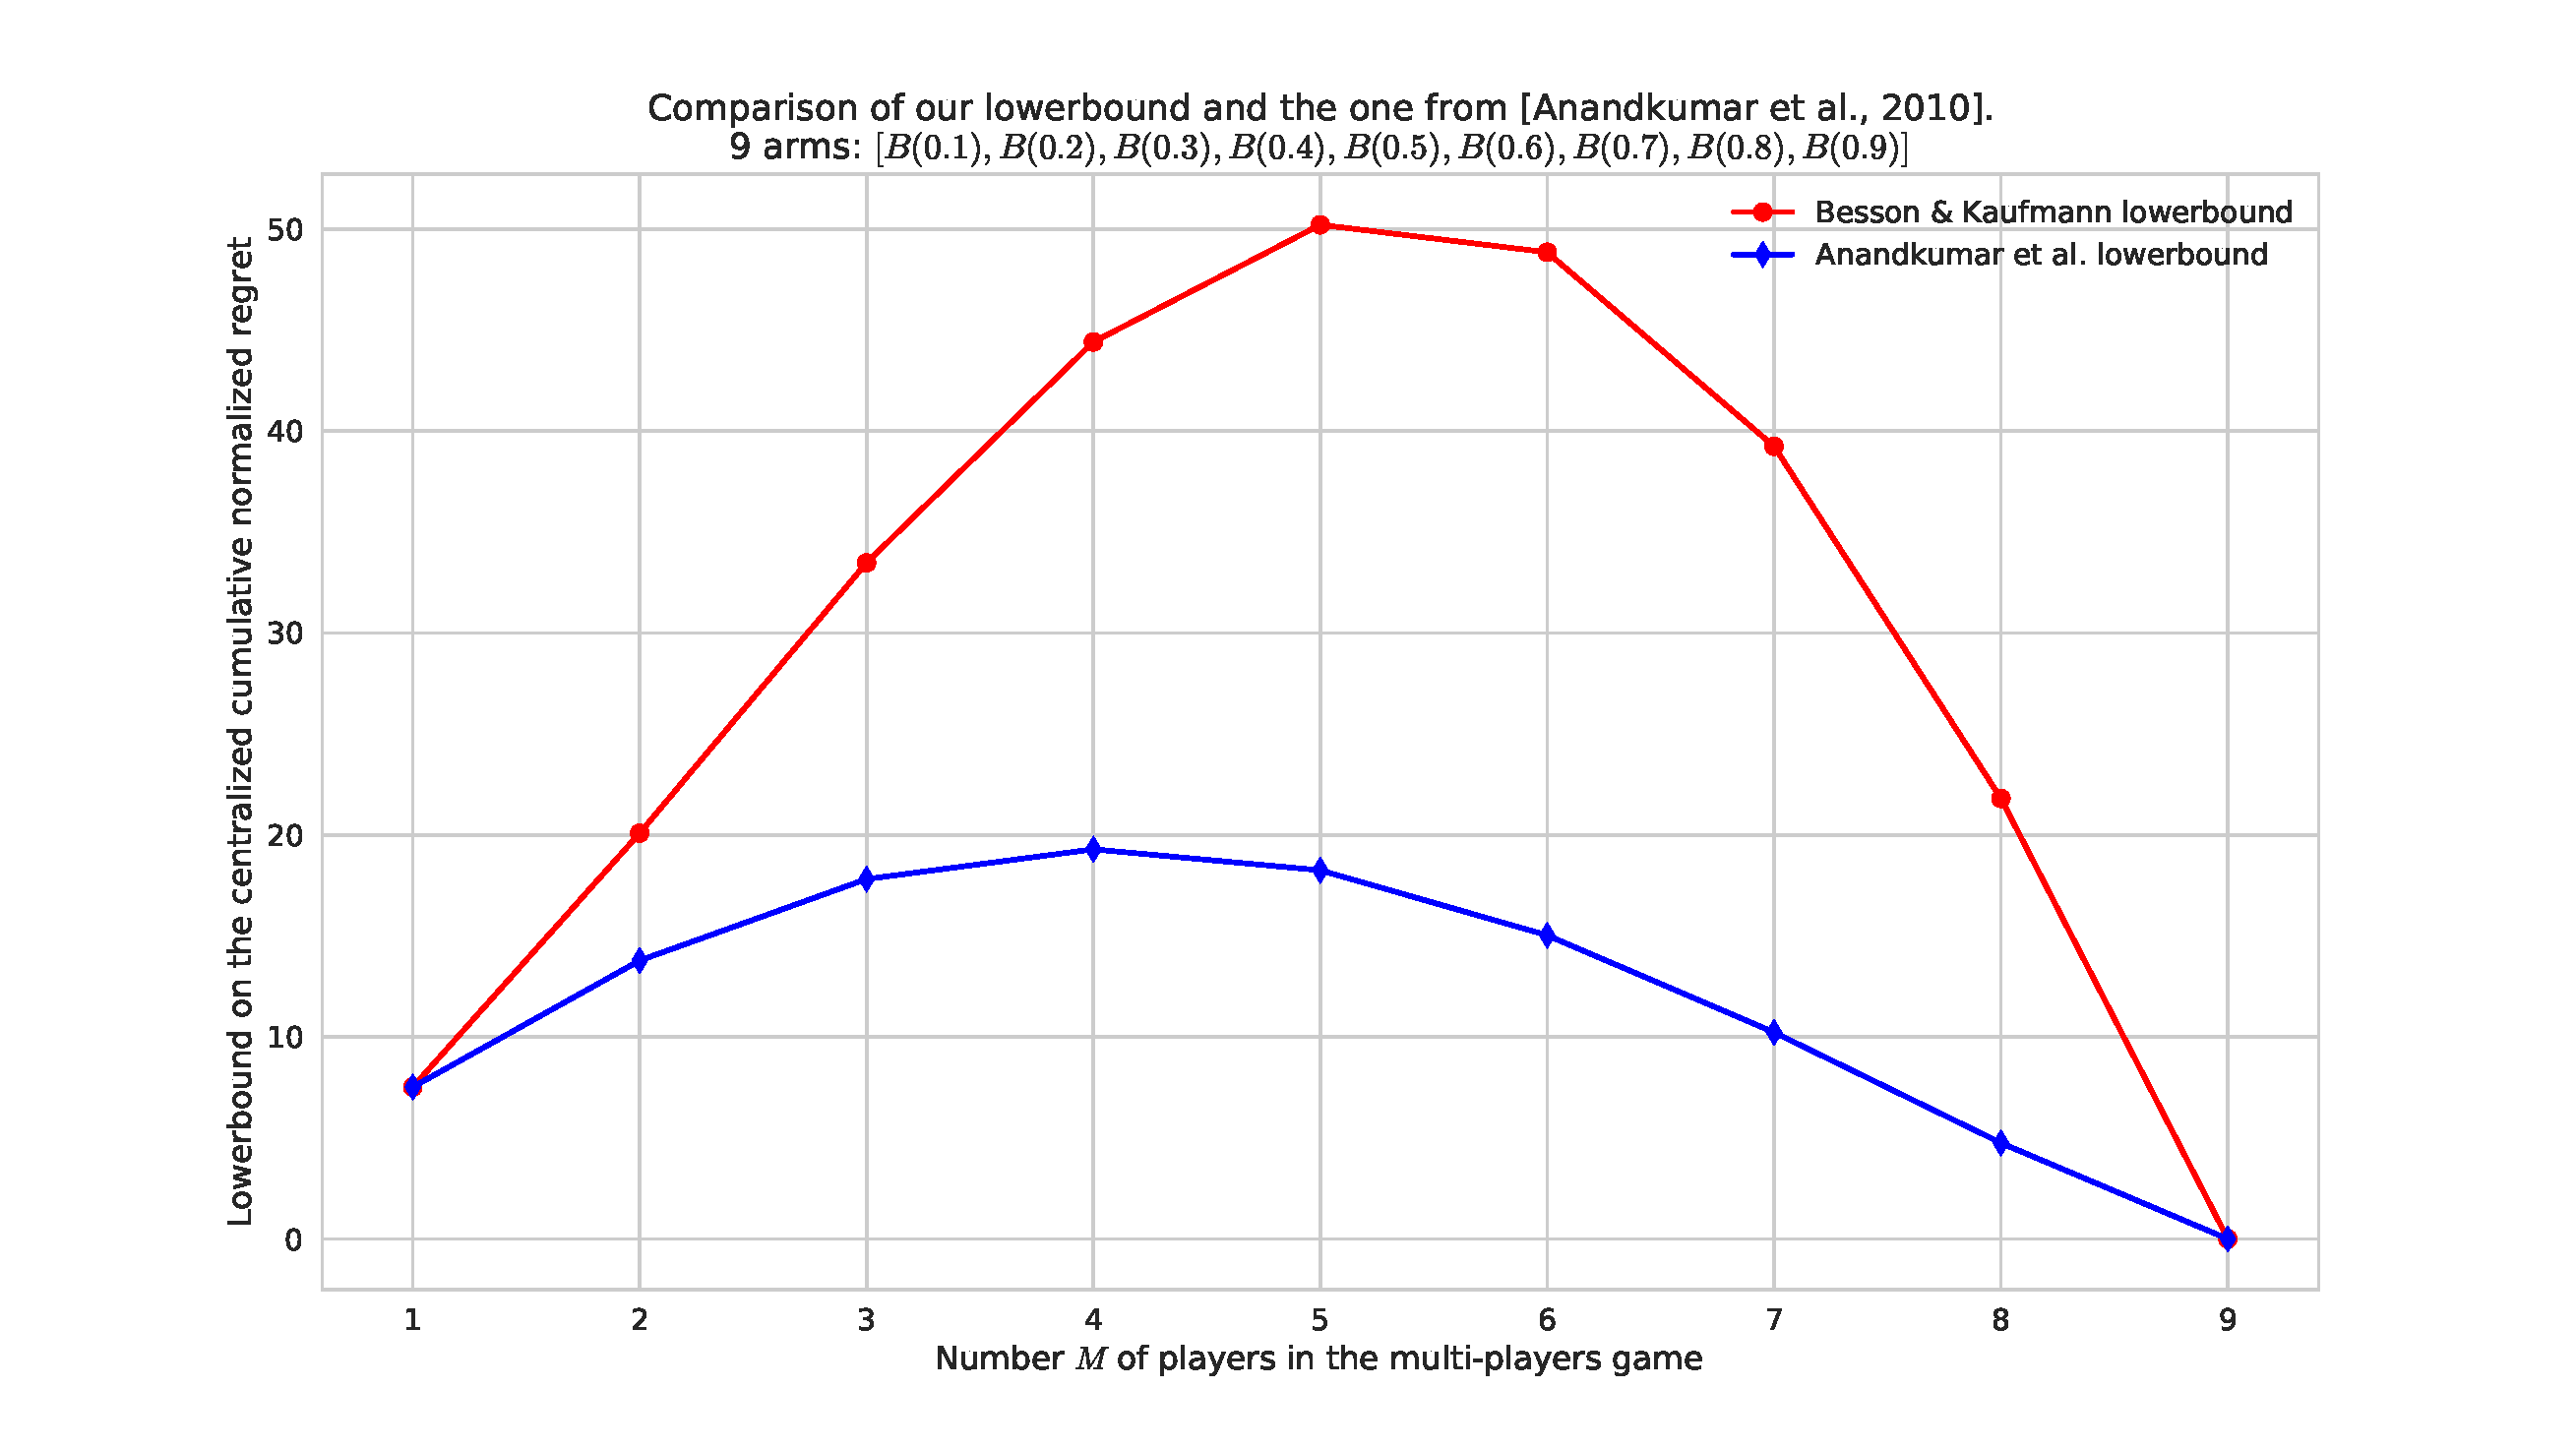
\includegraphics[width=0.70\textwidth]{Comparison_of_our_lowerbound_and_Anandkumar_2010__9_arms.pdf}
  \caption[Comparison of our lower bound against the one from \cite{Zhao10}]{Comparison of our lower bound against the one from \cite{Zhao10}, on a simple problem with $9$ Bernoulli arms, of means $\boldsymbol{\mu} = [0.1, 0.2, \dots, 0.9]$, as a function of the number of players $M$.}
  \label{fig:5:CompLowerBounds}
\end{figure}


%
% System regret and three terms
%
\begin{figure}[!h]
    \centering
    % \begin{subfigure}[!h]{1.00\textwidth}
        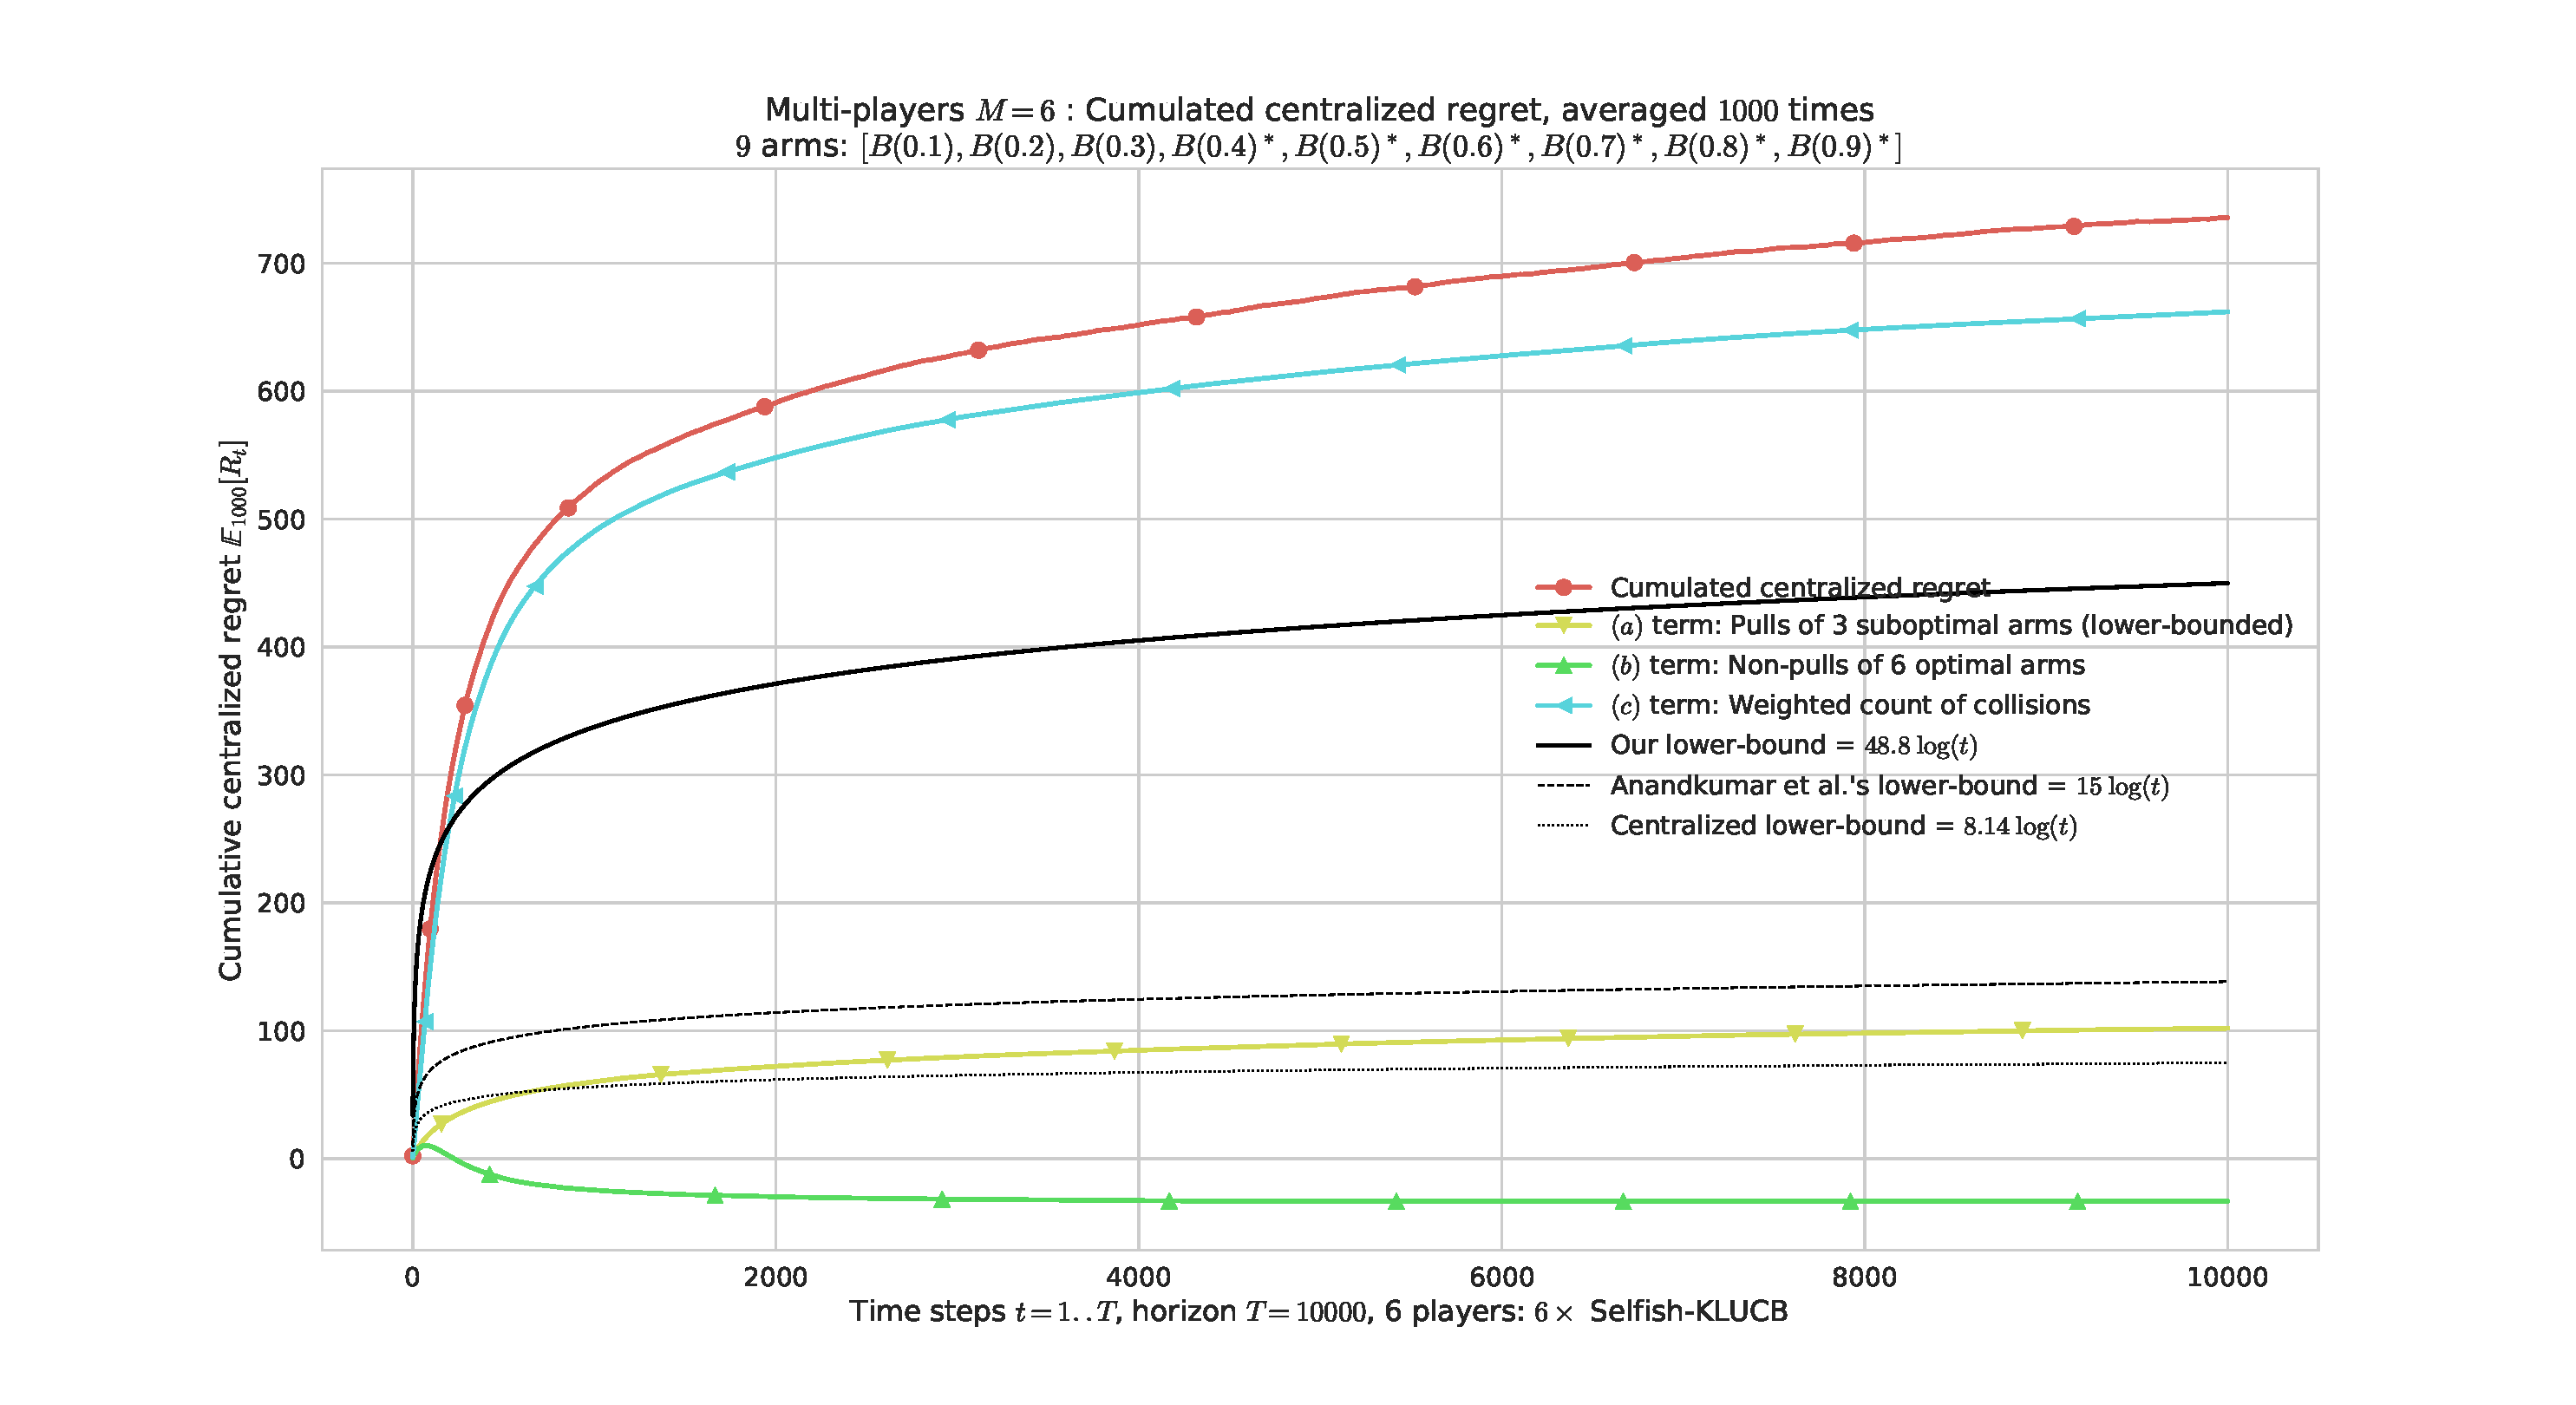
\includegraphics[width=1.00\textwidth]{main_RegretCentralized____env4-4_2092905764868974160.pdf}
    % \end{subfigure}
    % ~
    % \begin{subfigure}[!h]{1.00\textwidth}
        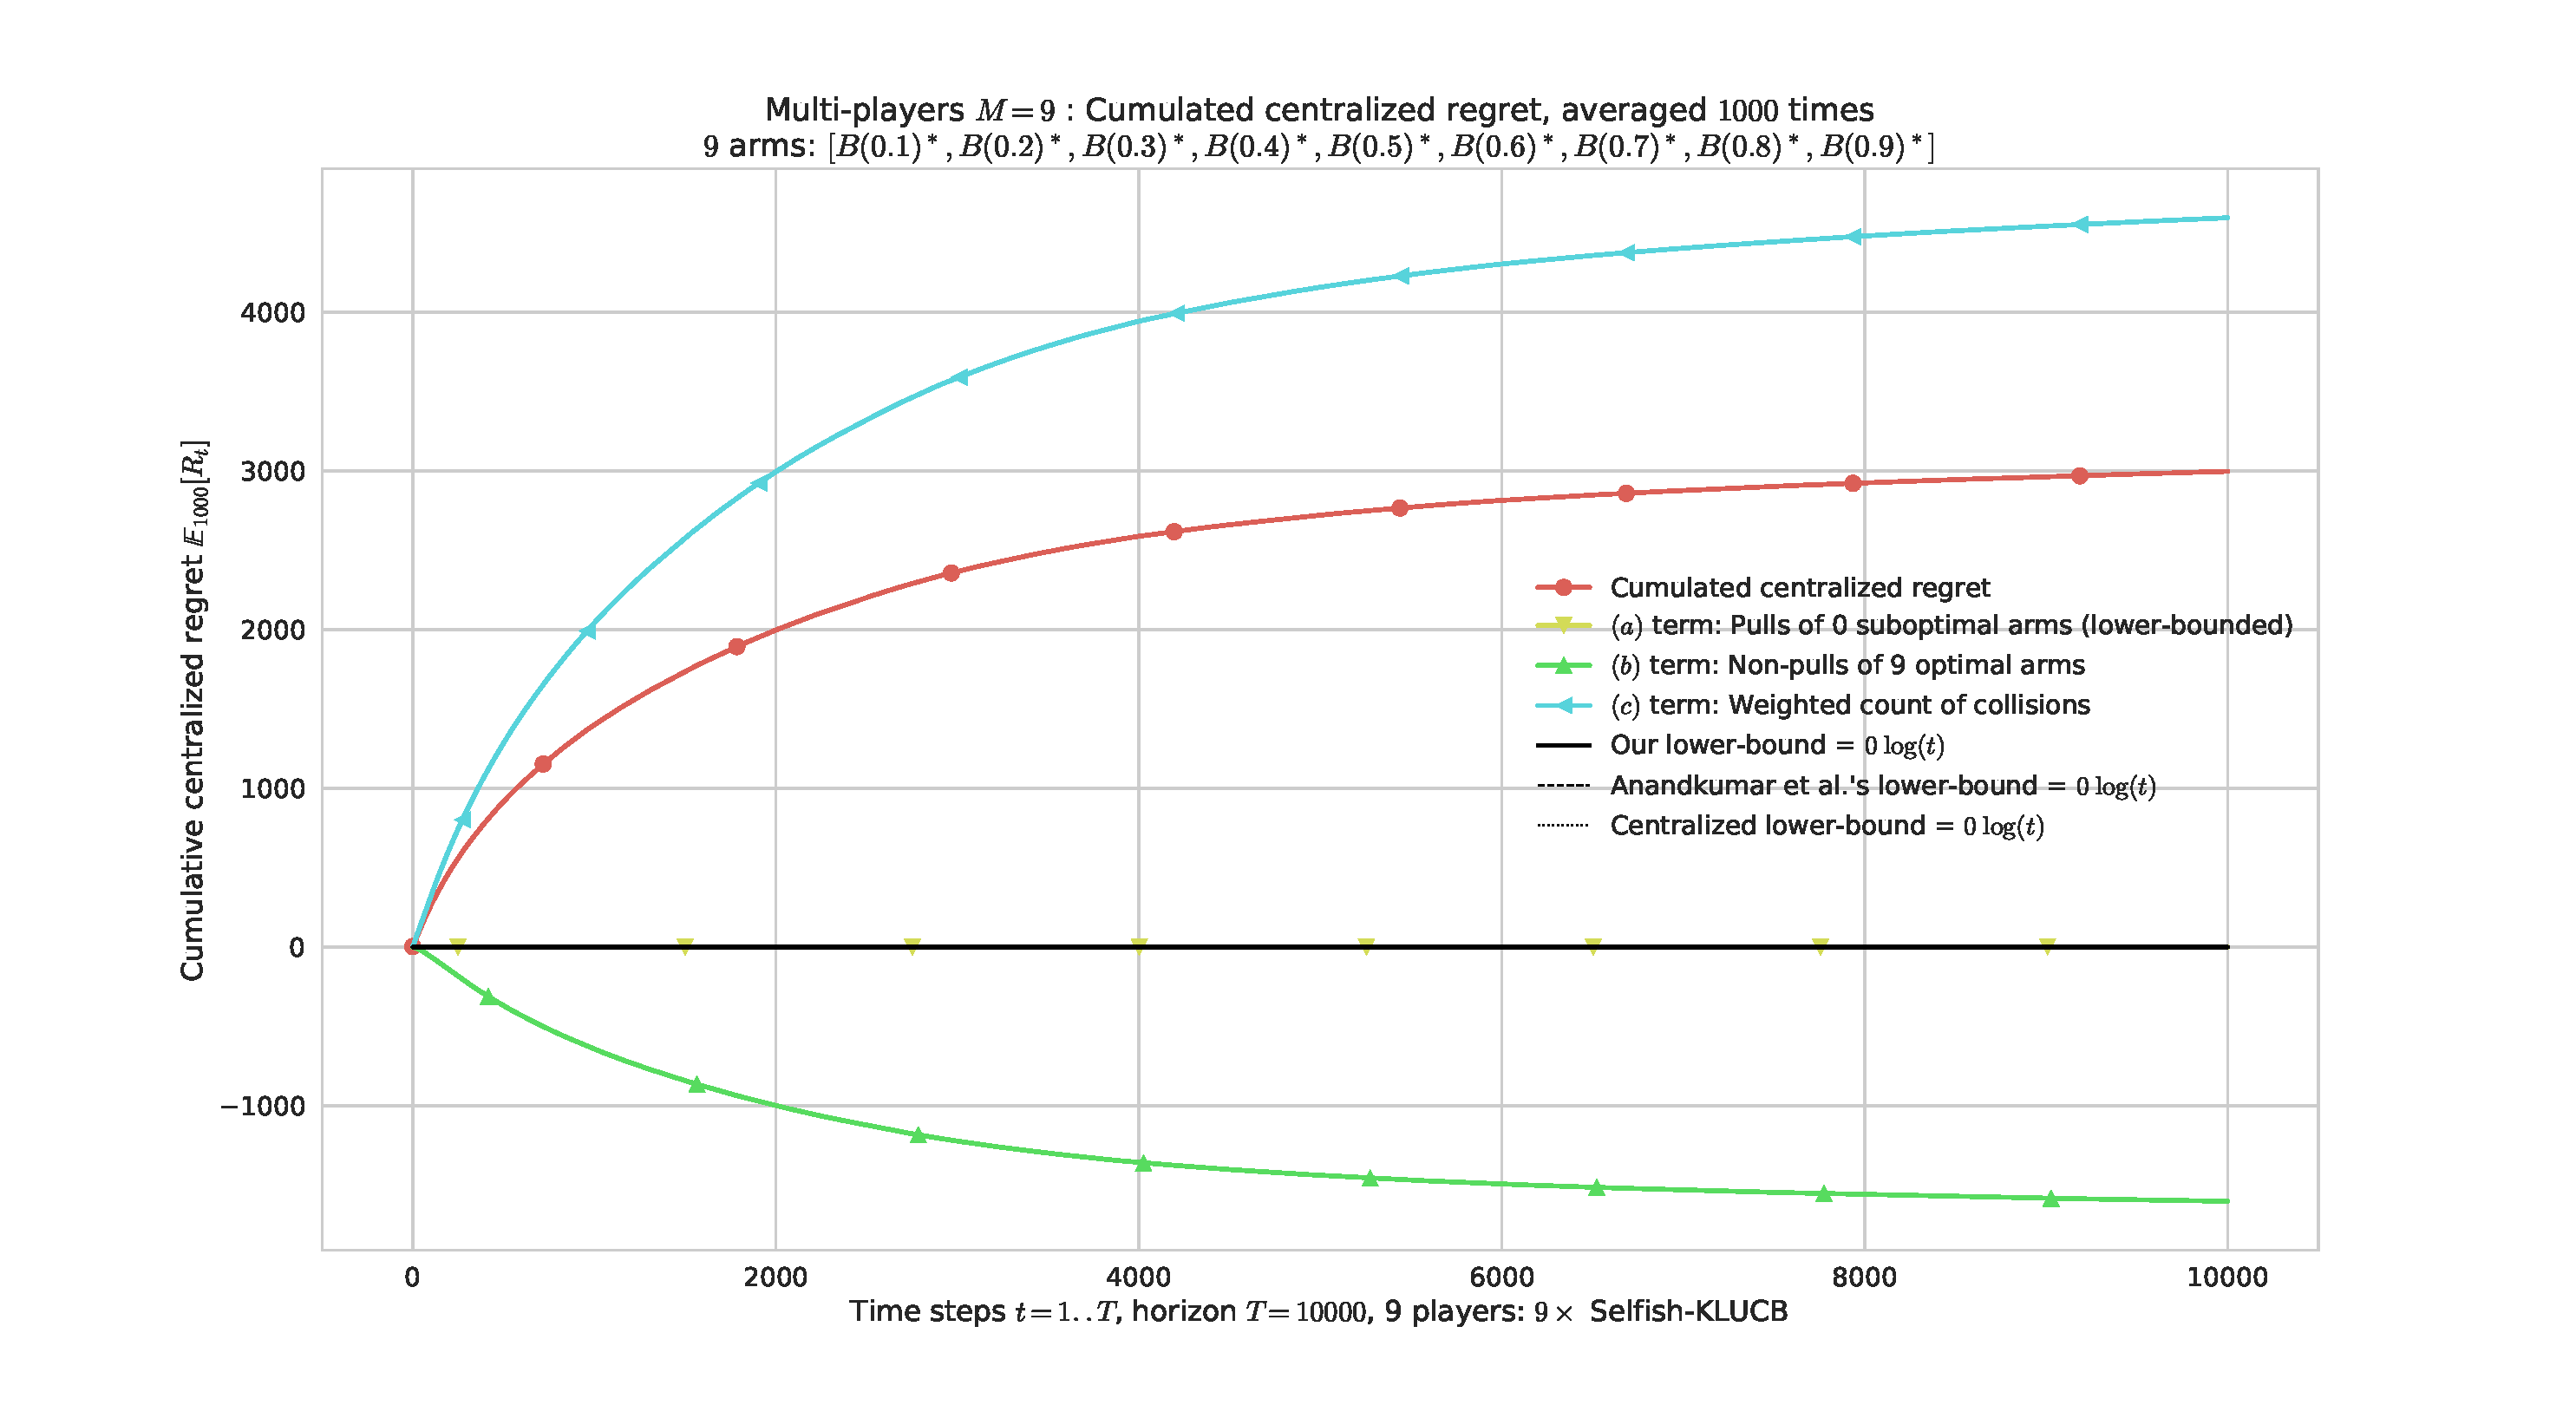
\includegraphics[width=1.00\textwidth]{main_RegretCentralized____env4-4_1699475021767911583.pdf}
    % \end{subfigure}
    \caption[Multi-player regret with its three terms]{Regret with its three terms \ref{eq:5:term1}, \ref{eq:5:term2}, \ref{eq:5:term3}, and lower bounds \eqref{eq:5:ourLowerBound} and \eqref{eq:5:Zhao10LowerBound} in \textbf{black}, for \Selfish-\klUCB: $M=6$ and $M=9$ players, $K=9$ arms, horizon $T=10000$ (for $1000$ runs).}
    \label{fig:5:MP__M9_K9_T10000_N1000__9_algos__main_RegretCentralized____env6}
    % \vspace*{-15pt}  % XXX remove if problem
\end{figure}



Figures~\ref{fig:5:MP__M9_K9_T10000_N1000__9_algos__main_RegretCentralized____env6}
show the regret $R_T(\boldsymbol{\mu}, M, \rho)$
on the same example problem $\boldsymbol{\mu}$, with $K = 9$ arms and respectively $M = 6$, or $9$ players, for \Selfish-\klUCB.
%
It is just a simple way to check that the two lower bounds on the regret indeed appear as valid lower bounds empirically,
and are moreover lower bounds on the count of selections (\ref{eq:5:term1}, displayed in \textcolor{blue}{cyan}).
%
The lower bounds (in black) are $C(\boldsymbol{\mu}, M) \log t$, the dashed line
for \citeauthor{Zhao10}'s lower bound, and the continuous line is our lower bound.
%
These plot show the regret (in red),
% the three lower bounds
% (centralized, \citeauthor{Anandkumar11}'s and our lower bounds, in black),
and the three terms \ref{eq:5:term1}, \ref{eq:5:term2}, \ref{eq:5:term3} in the decomposition of the regret.
As explained in Lemma~\ref{lem:5:DecompositionRegret}, term \ref{eq:5:term2} is not always non-negative.
For $M=9$ and \Selfish, \ref{eq:5:term3} is actually larger than the regret,
and term \ref{eq:5:term1} is zero, as well as the lower bounds.


\subsection{Figures from Section~\ref{sec:5:experiments}}
\label{app:5:plotsFromSec5}

This last Appendix includes the figures used in Section~\ref{sec:5:experiments},
with additional comments.


\begin{figure}[!h]
    \centering
    % \begin{subfigure}[!h]{0.85\textwidth}
        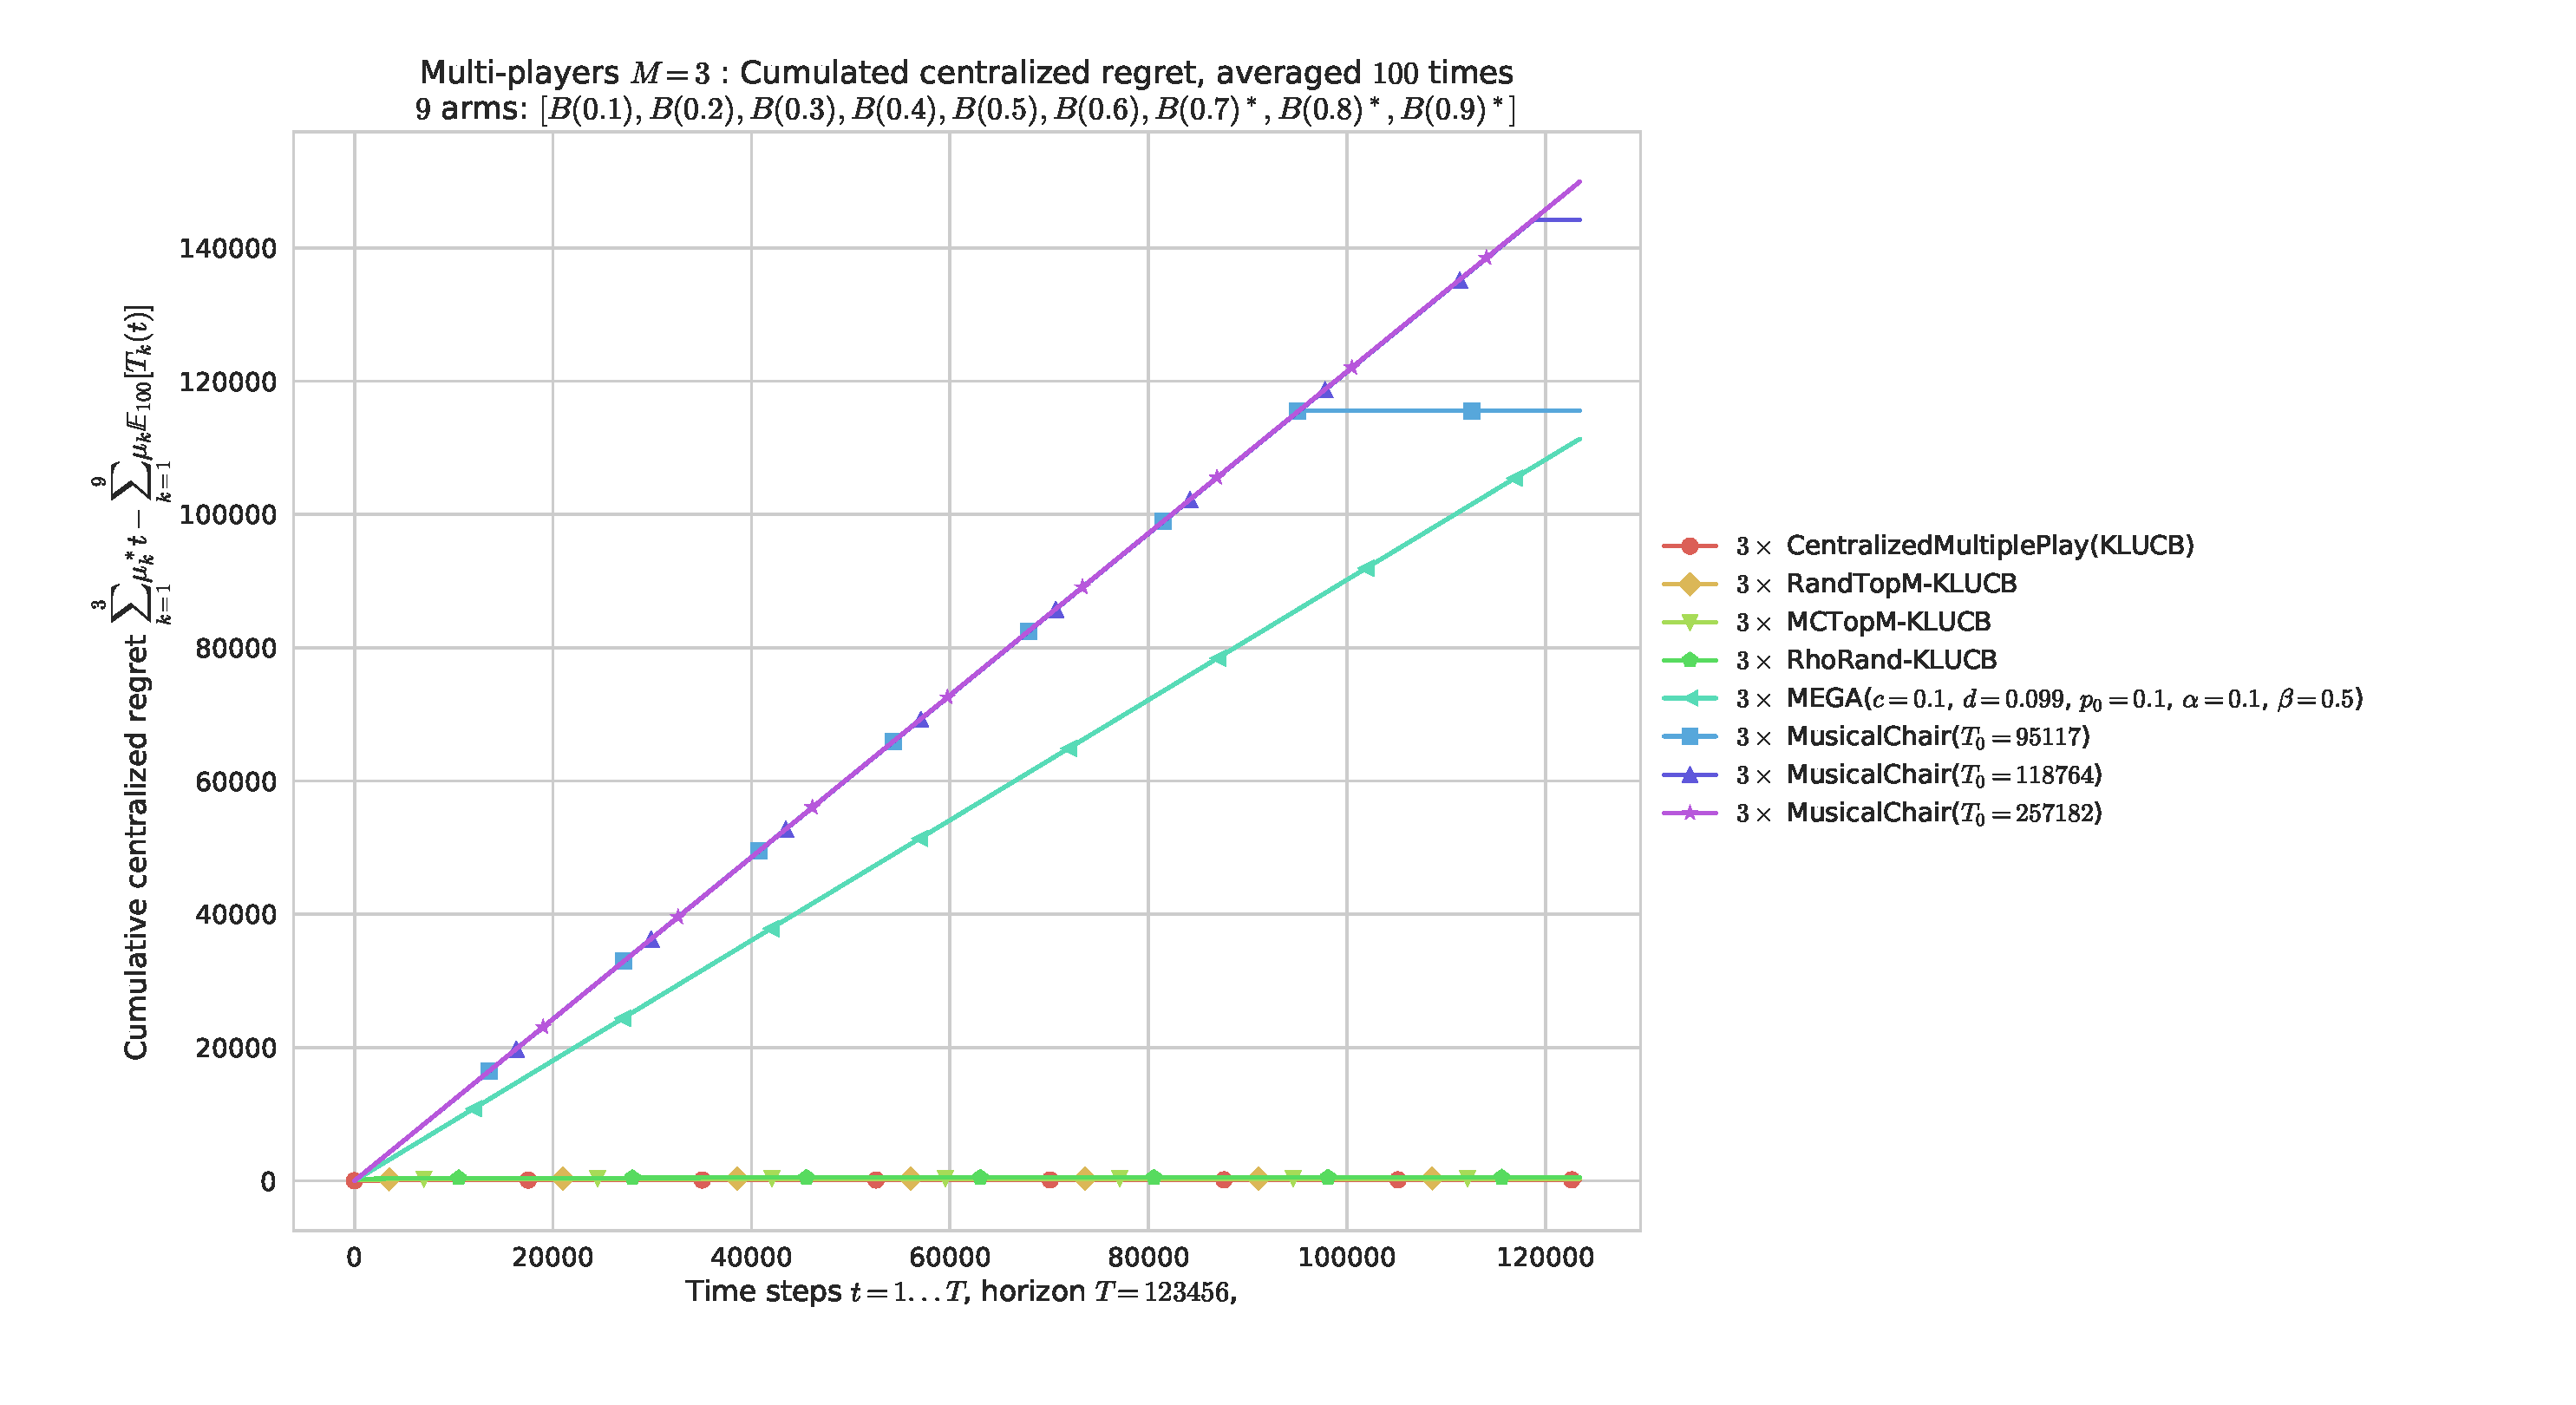
\includegraphics[width=1.00\textwidth]{MP__K9_M3_T123456_N100__8_algos/all_RegretCentralized____env1-1_7803645526012310577.pdf}
    % \end{subfigure}
    % ~
    % \begin{subfigure}[!h]{0.85\textwidth}
        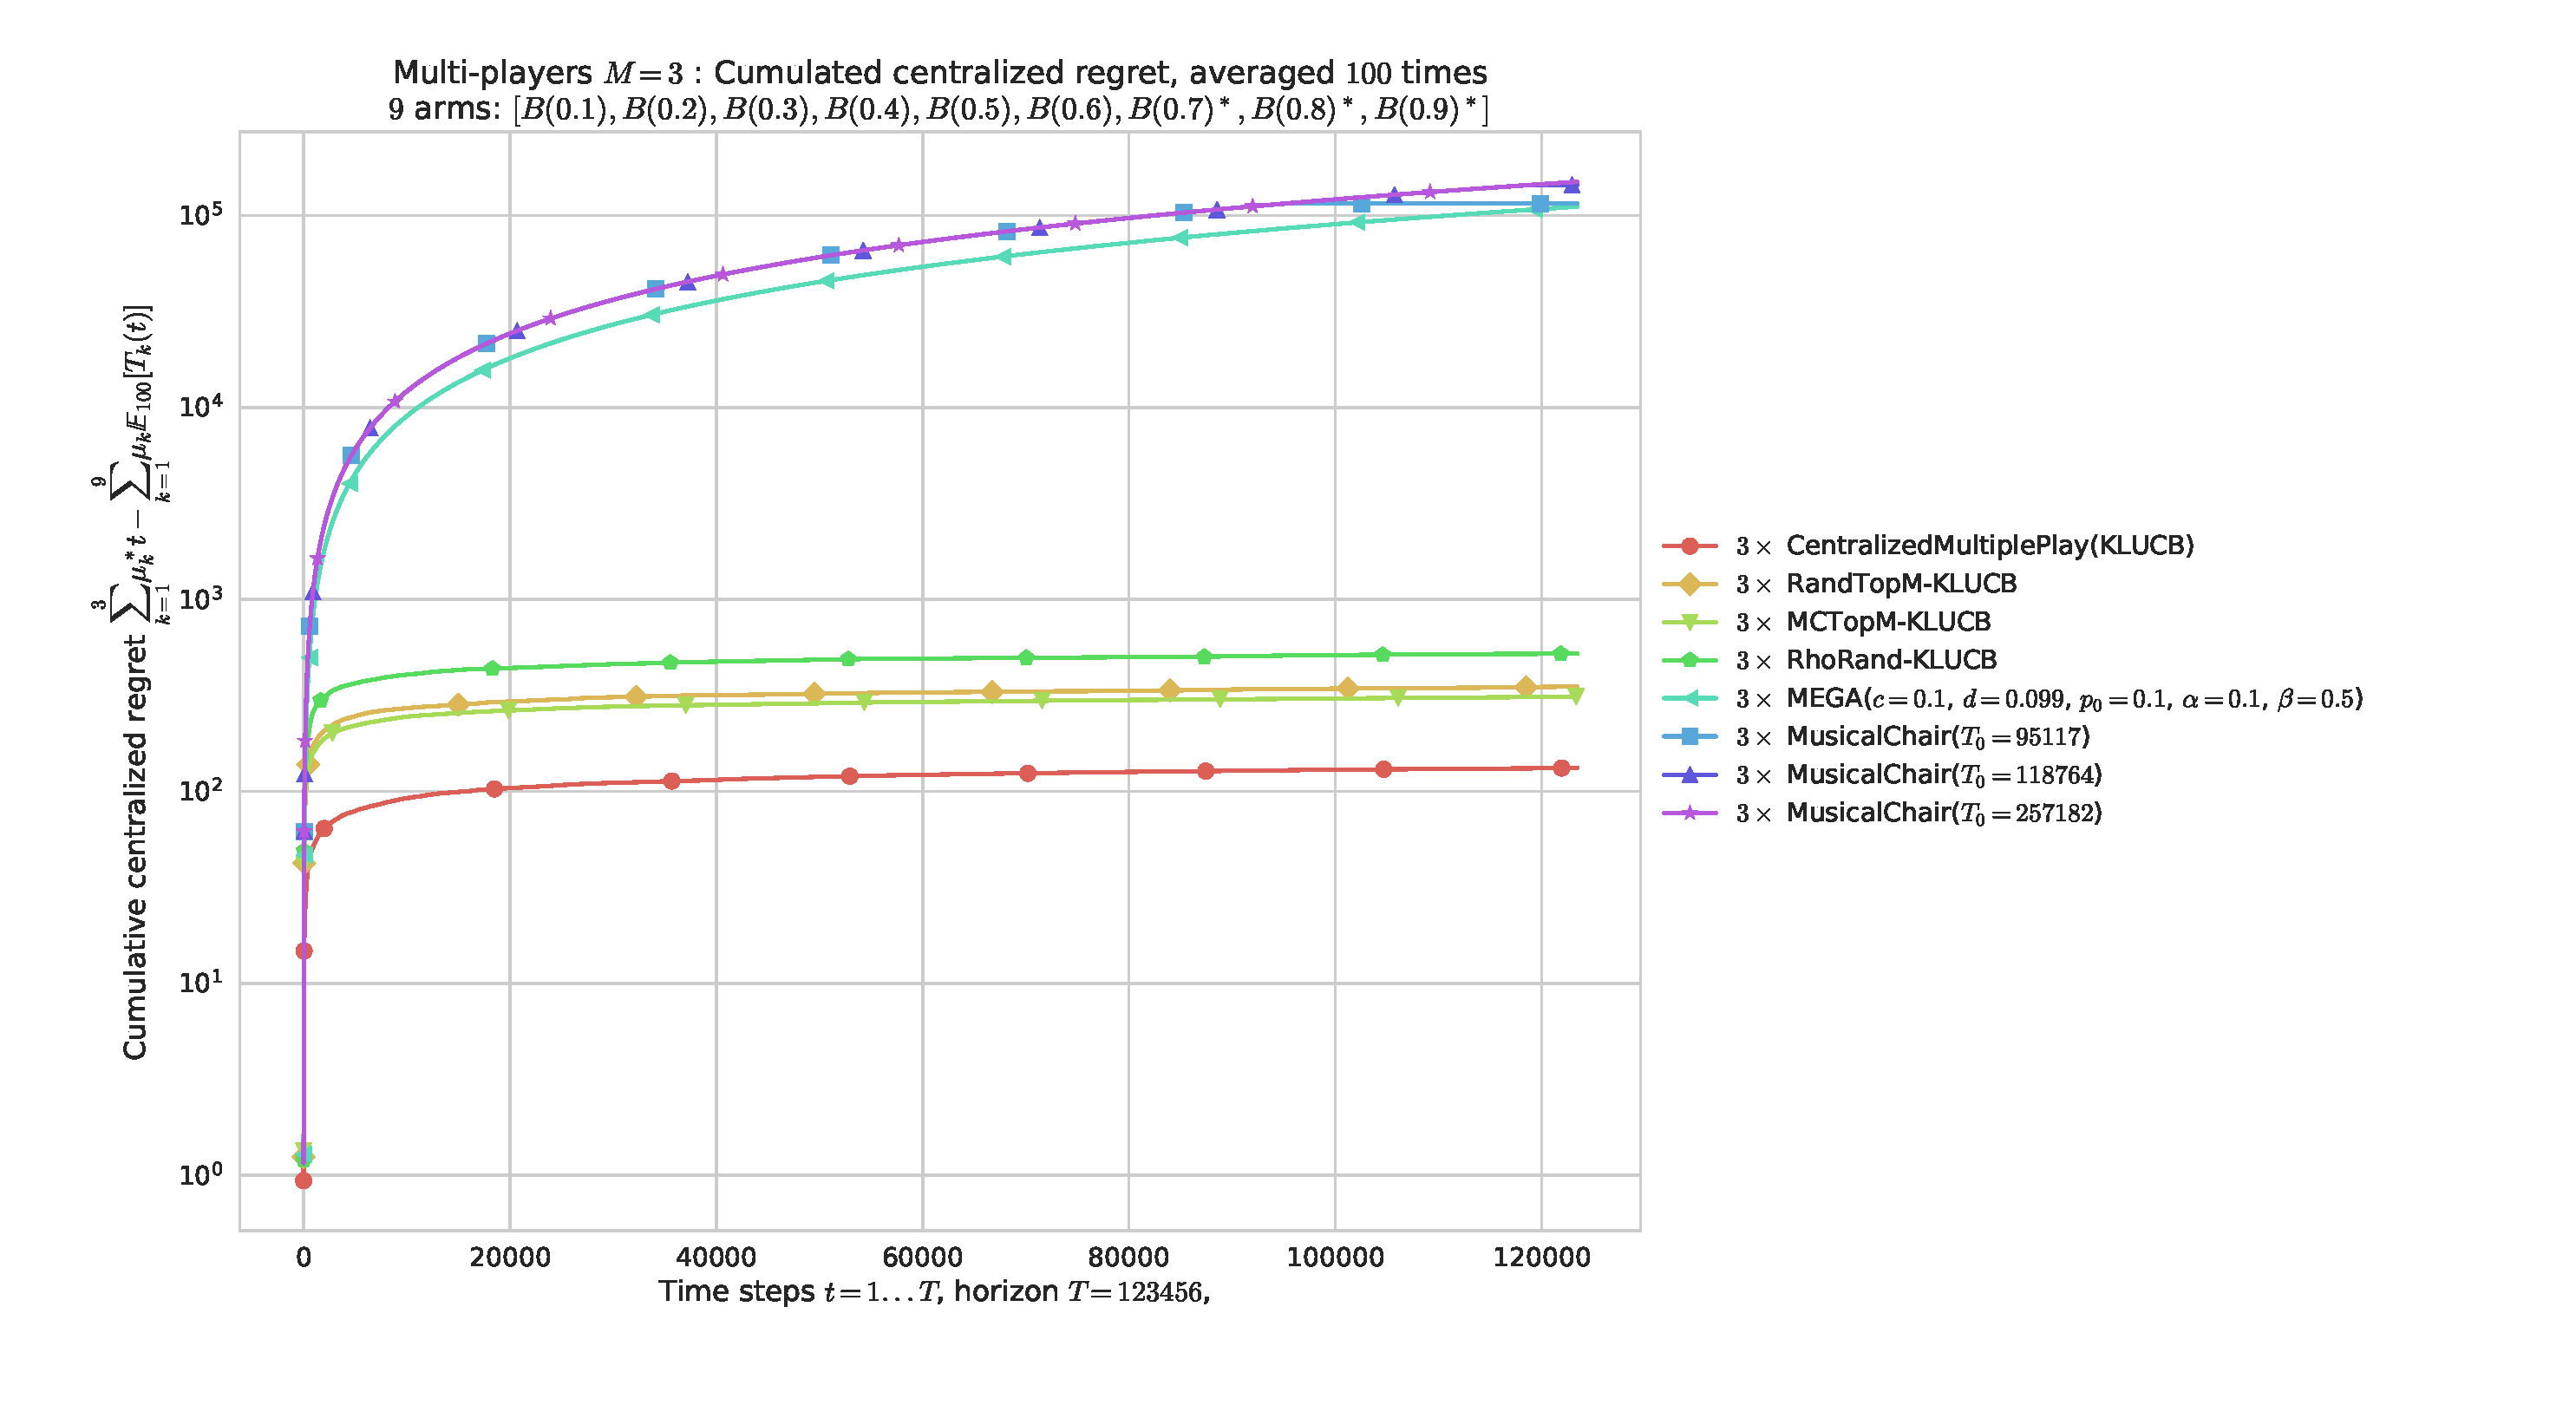
\includegraphics[width=1.00\textwidth]{MP__K9_M3_T123456_N100__8_algos/all_RegretCentralized_semilogy____env1-1_7803645526012310577.pdf}
    % \end{subfigure}
    \caption[Regret for $M=3$ players for $K=9$ arms, horizon $T=123456$, for $100$ repetitions on a fixed problem]{Regret (in log-$y$ scale on the right) for $M=3$ players for $K=9$ arms, horizon $T=123456$, for $100$ repetitions on problem $\mu=[0.1,\dots,0.9]$. With a perfect knowledge on the gap ($\Delta=0.1$ here) and by using the parameters suggested from their respective articles, \MEGA{} and \MusicalChair{} perform badly in this simple setting, even with the knowledge of the horizon $T$ for \MusicalChair{}. The first two \MusicalChair{} instances use the optimal $T_0$ value from \cite{Rosenski16}, with $\varepsilon$ taken slightly smaller than the gap $\Delta$ ($\varepsilon=0.99 \Delta$), and respectively with $\delta=0.5$ and $\delta=0.1$, for which the regret can bounded with probability $0.5$ and $0.9$ respectively. The third instance uses the optimal $T_0$ corresponding to $\delta=1/T$, that is guaranteed to have an expected regret of order $\log(T)$.}
    \label{fig:5:MP__K9_M3_T123456_N100__8_algos}
\end{figure}

%
% Regular plots of centralized regrets
%
\begin{figure}[!h]
    \centering
    % \begin{subfigure}[!h]{0.49\textwidth}
        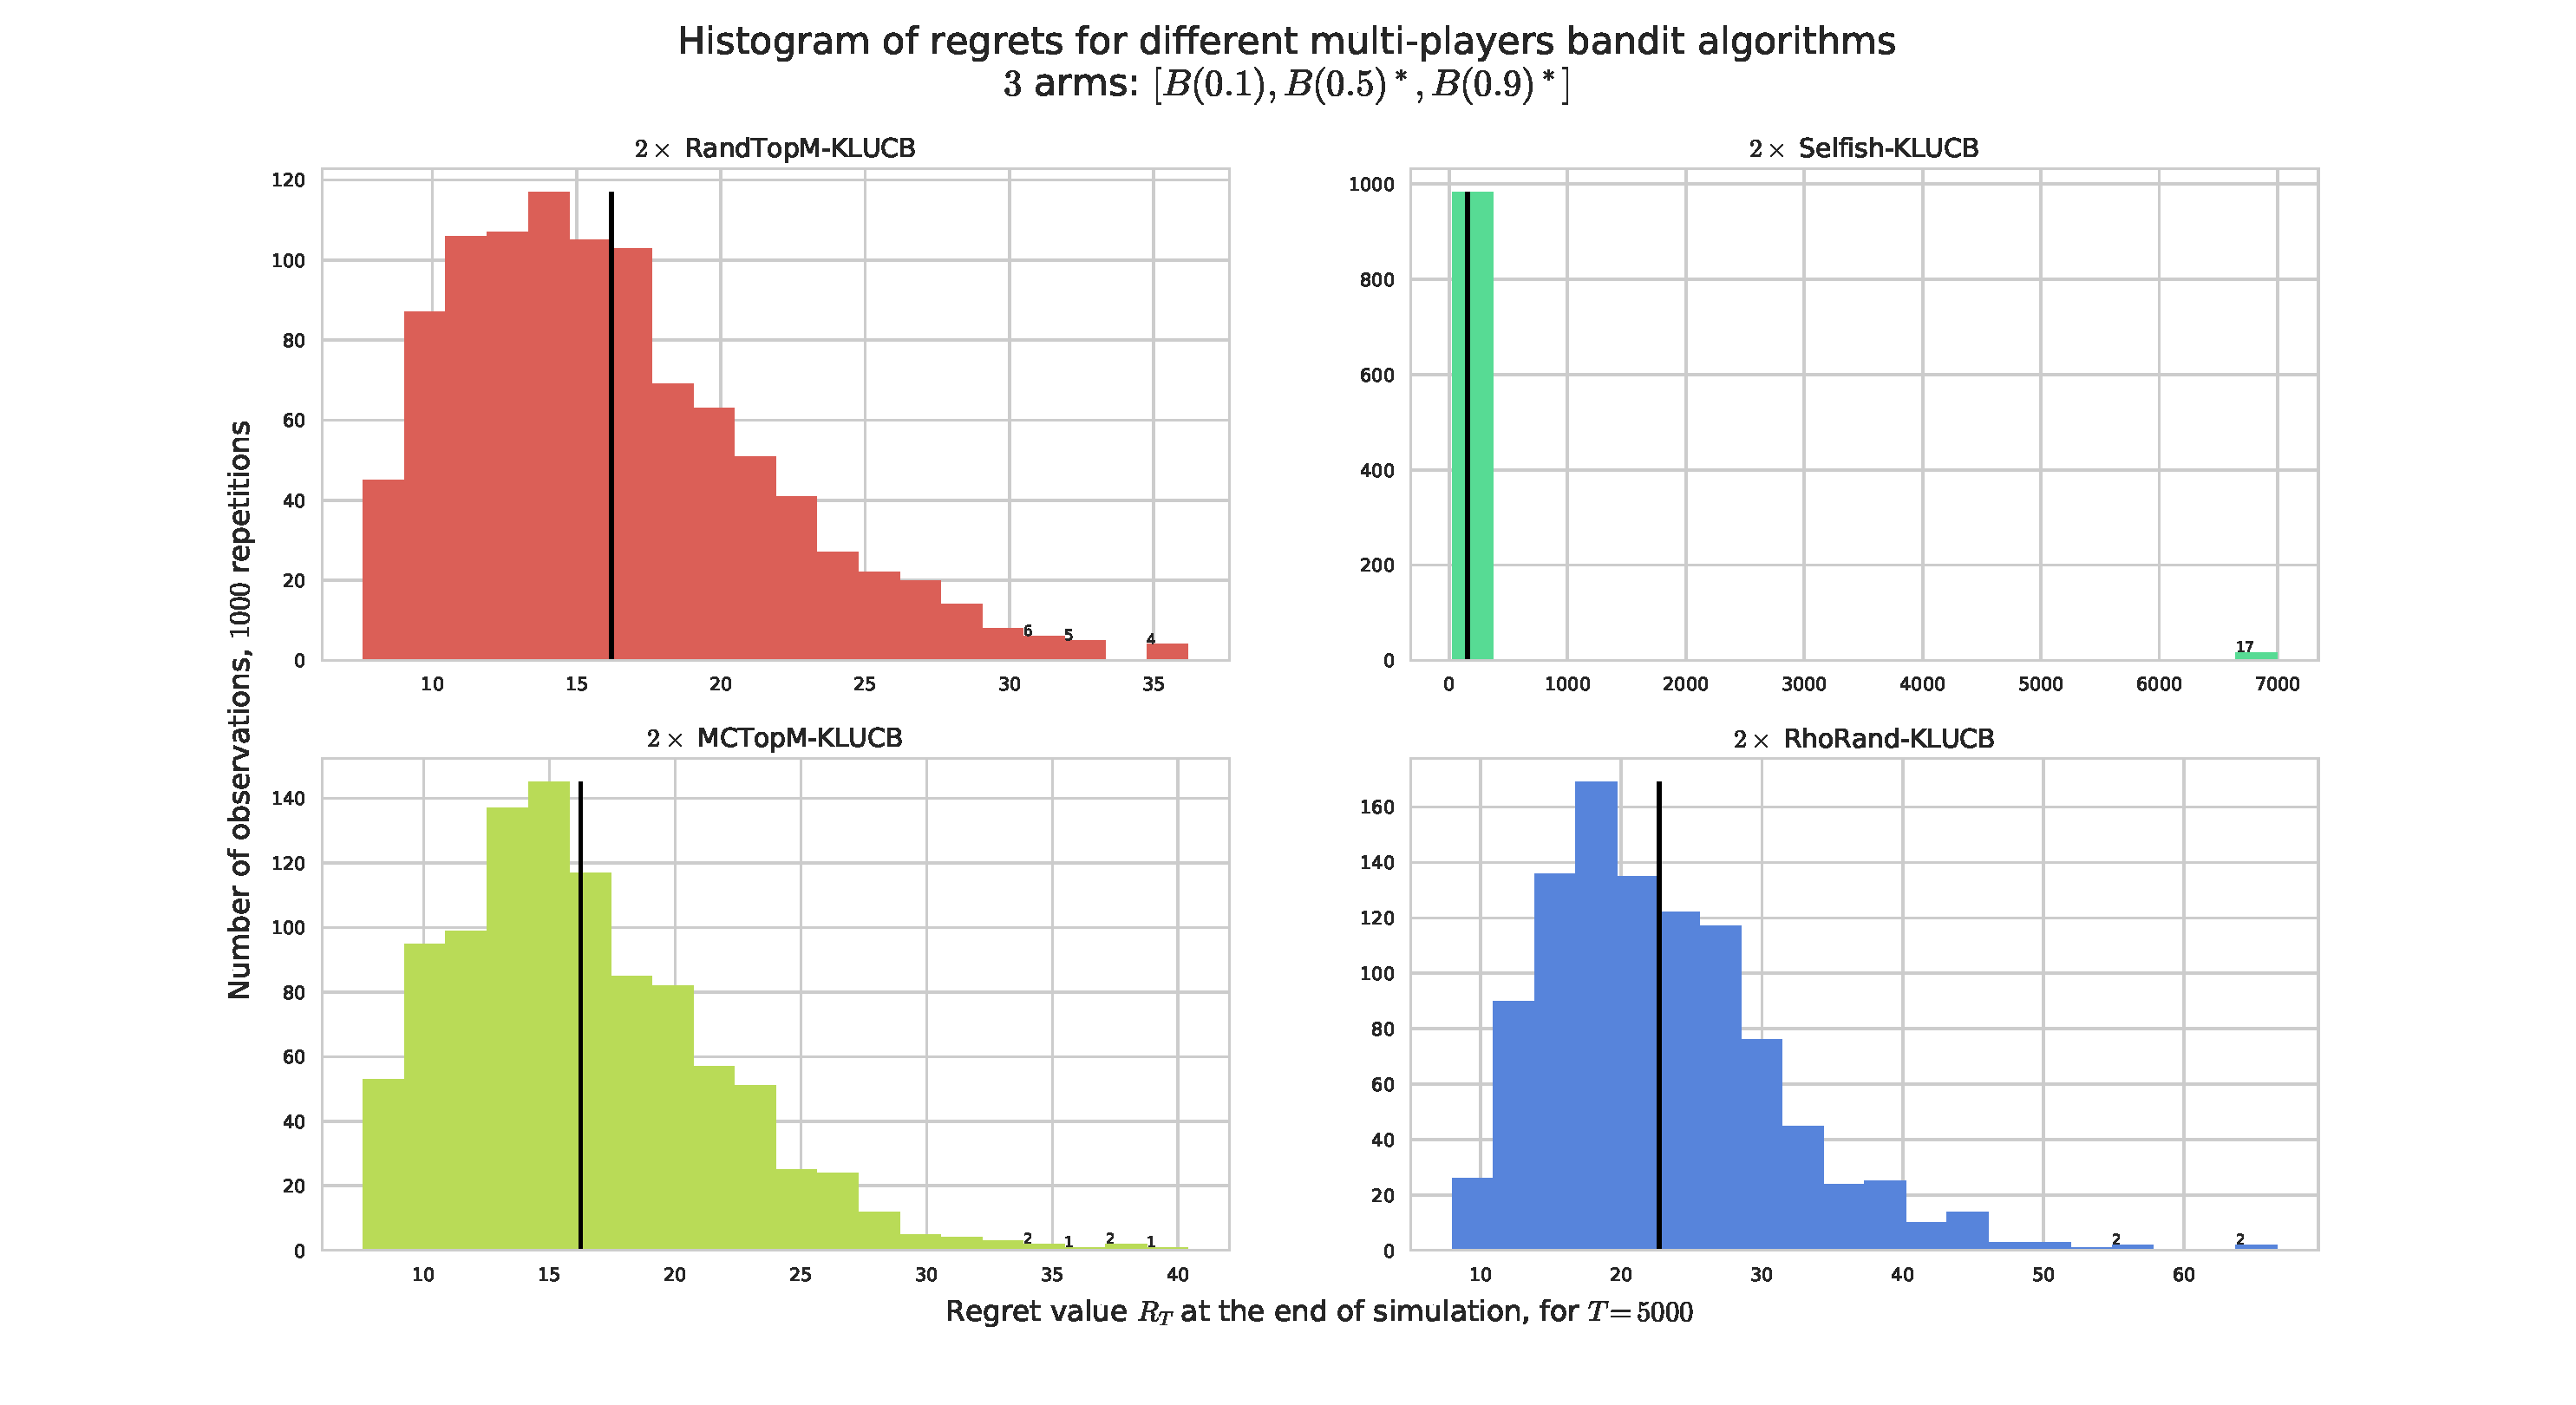
\includegraphics[width=0.90\textwidth]{MP__K3_M2_T5000_N1000__4_algos/all_HistogramsRegret____env1-1_5016720151160452442.pdf}
    % \end{subfigure}
    % % ~
    % \begin{subfigure}[!h]{0.49\textwidth}
    %   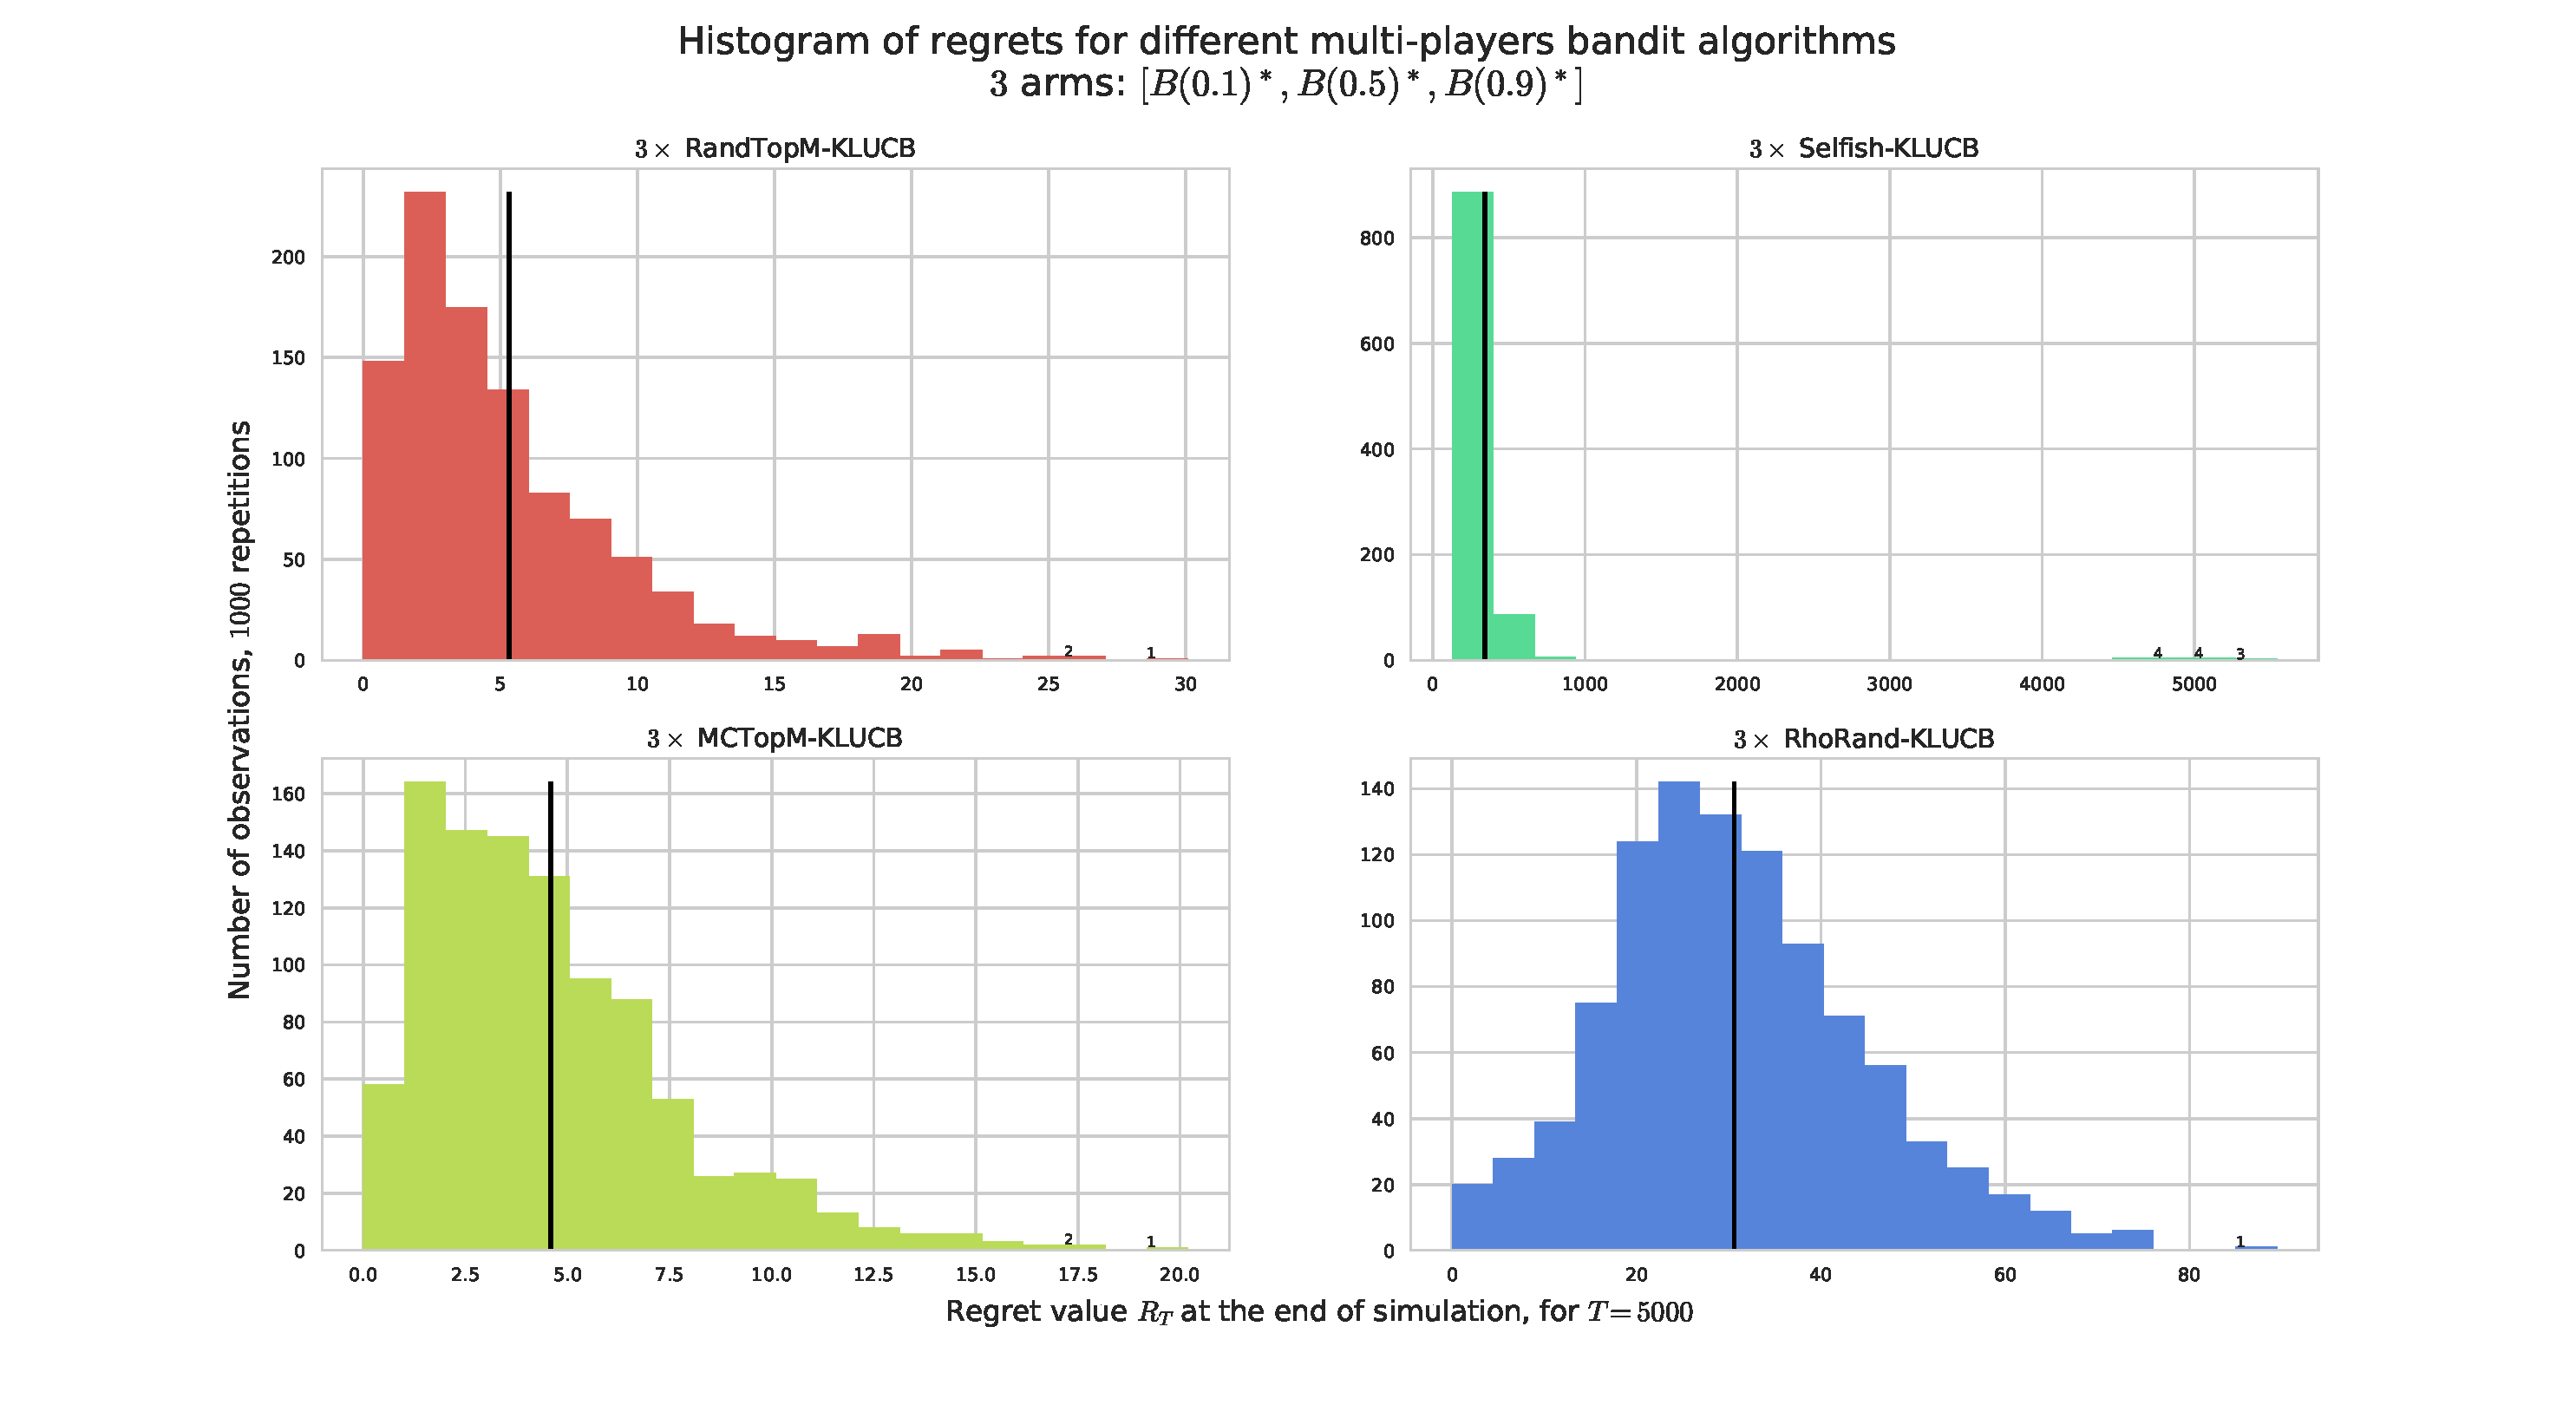
\includegraphics[width=1.10\textwidth]{MP__K3_M3_T5000_N1000__4_algos/all_HistogramsRegret____env1-1_1035303196230283176.pdf}
    % \end{subfigure}
    \caption[Failure case of \Selfish]{Regret for $M=2$ players, $K=3$ arms, horizon $T=5000$, $1000$ repetitions and $\boldsymbol{\mu} = [0.1, 0.5, 0.9]$. Axis $x$ is for regret (different scale for each part), and the \textcolor{darkgreen}{green} curve for \Selfish{} shows a small probability of having a linear regret ($17$ cases of $R_T \geq T$, out of $1000$). The regret for the three other algorithms is very small for this problem, always smaller than $100$ here.}
    \label{fig:5:selfish_fail1}
    % \vspace*{-15pt}  % XXX remove if problem
\end{figure}


%
% Regular plots of centralized regrets
%
\begin{figure}[!h]
    \centering
    % \begin{subfigure}[!h]{0.49\textwidth}
        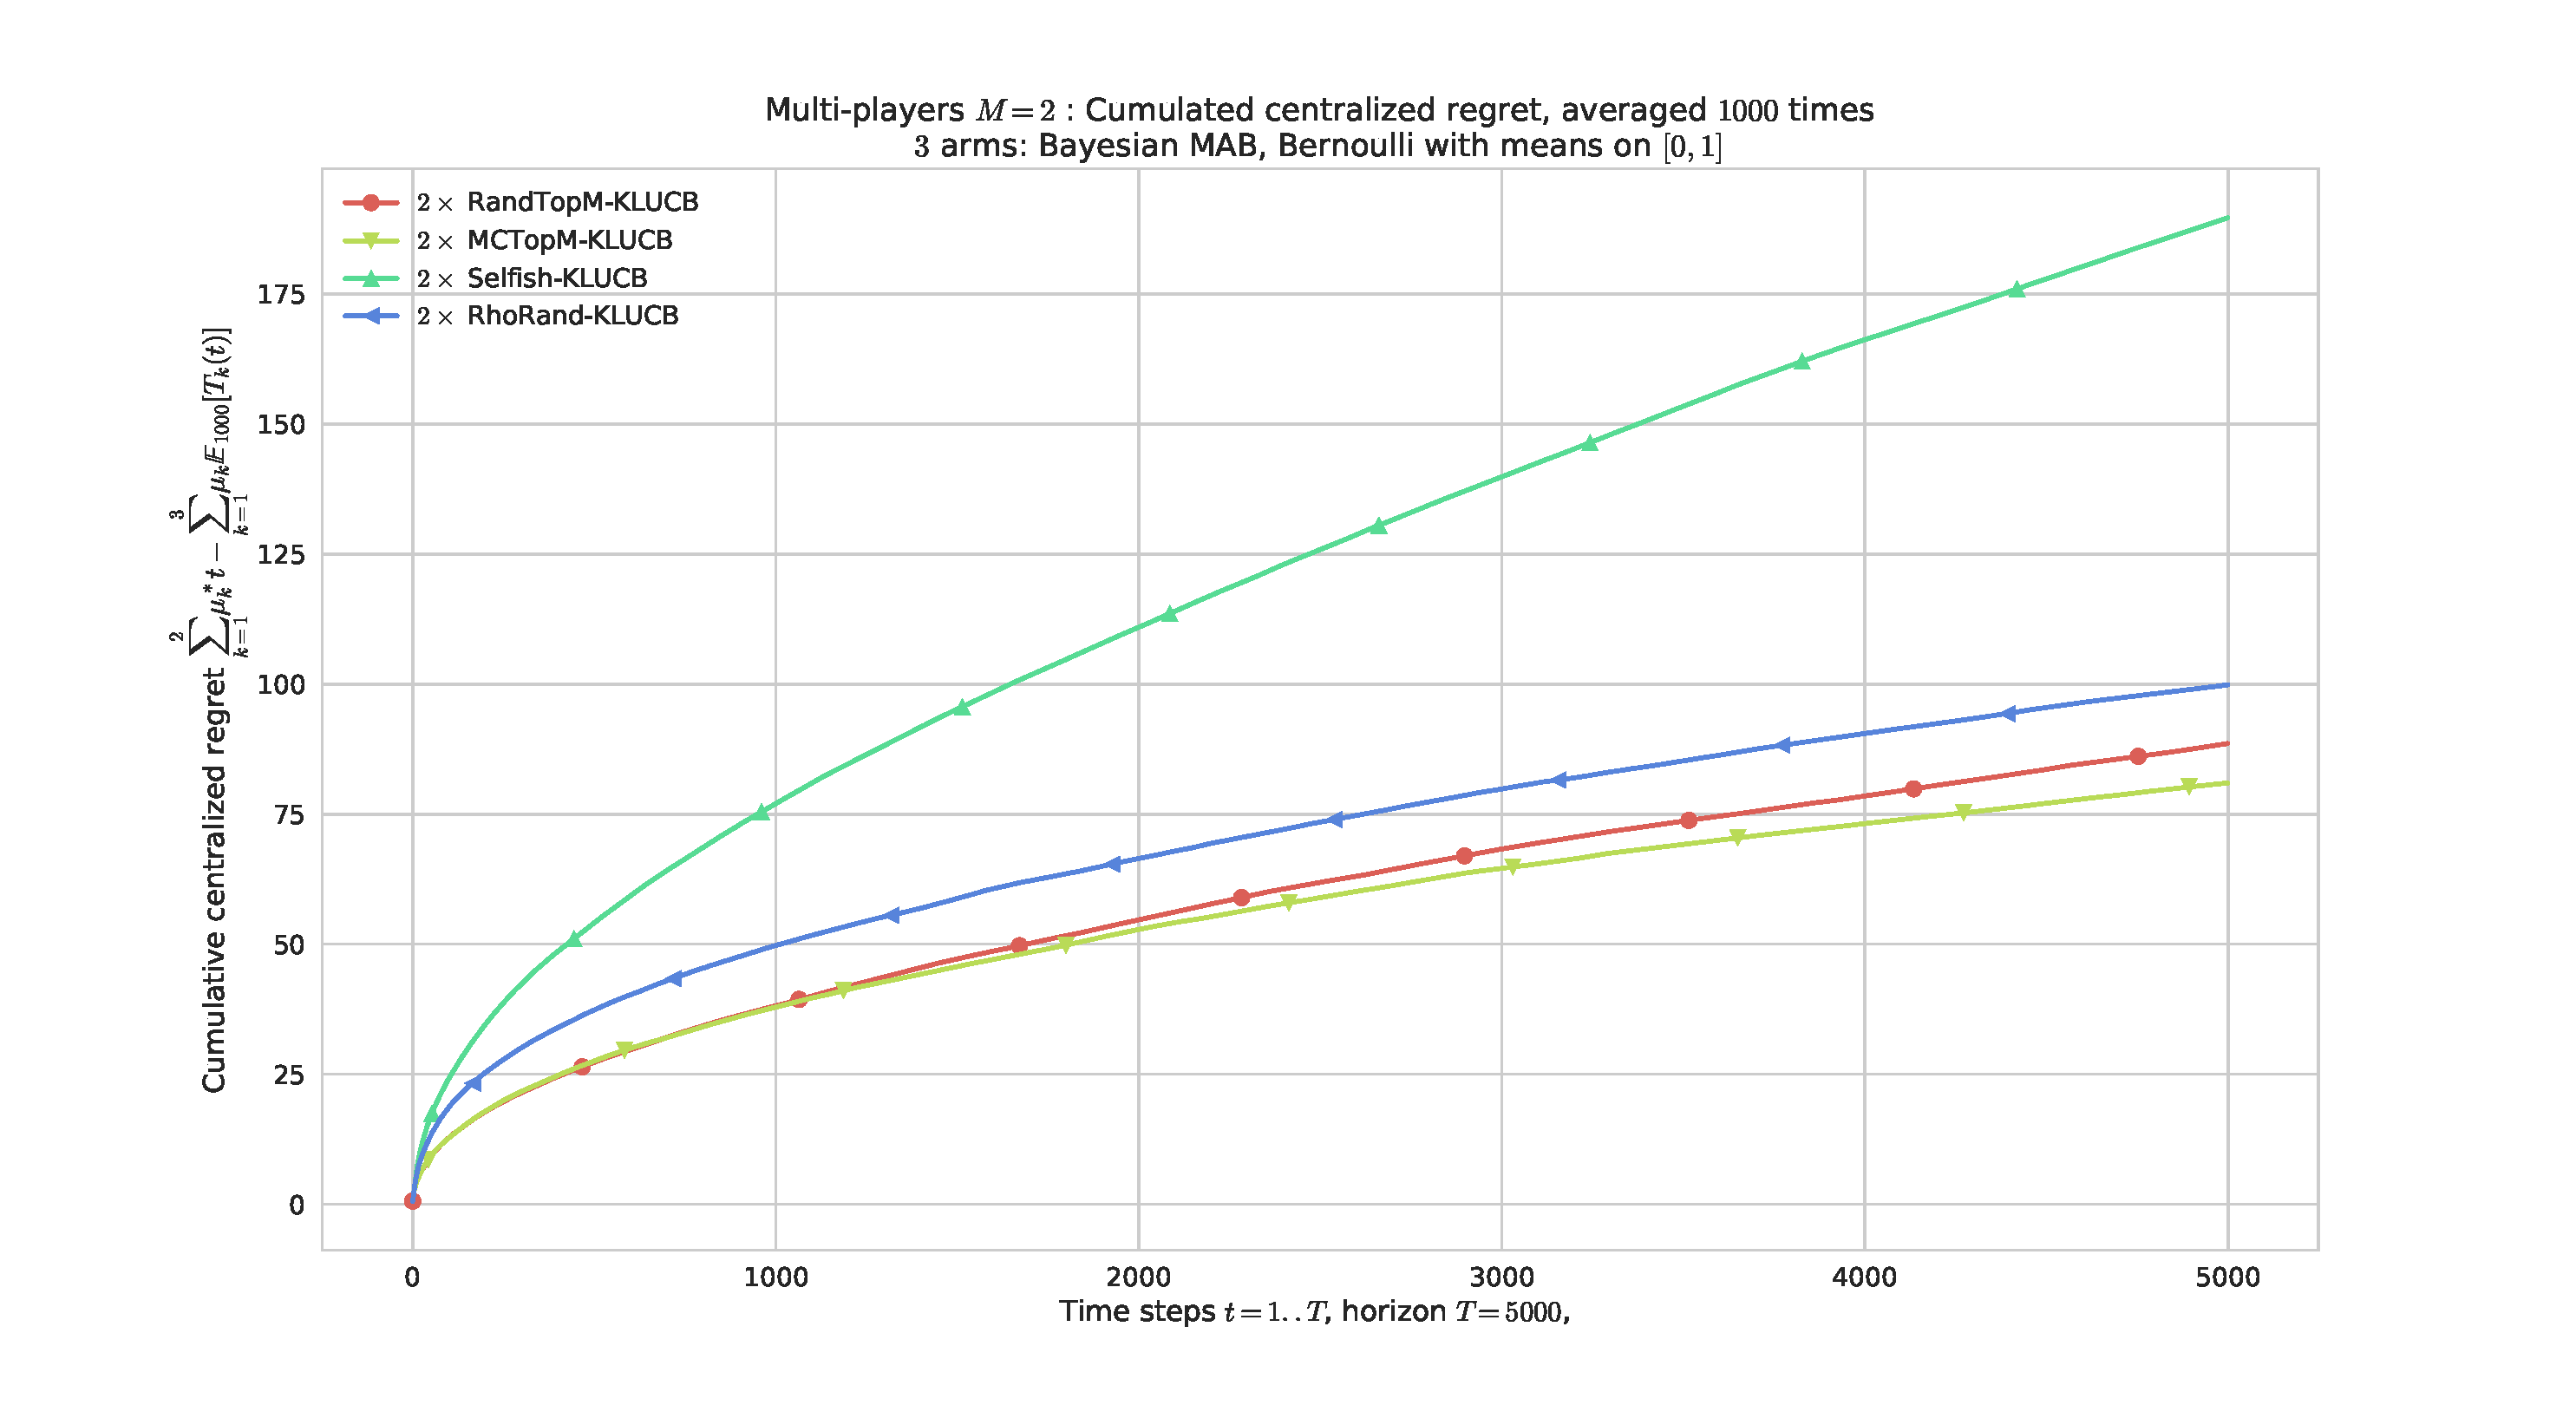
\includegraphics[width=1.00\textwidth]{MP__K3_M2_T5000_N1000__4_algos/all_RegretCentralized____env1-1_2643560344649862285.pdf}
    % \end{subfigure}
    % ~
    % \begin{subfigure}[!h]{0.49\textwidth}
        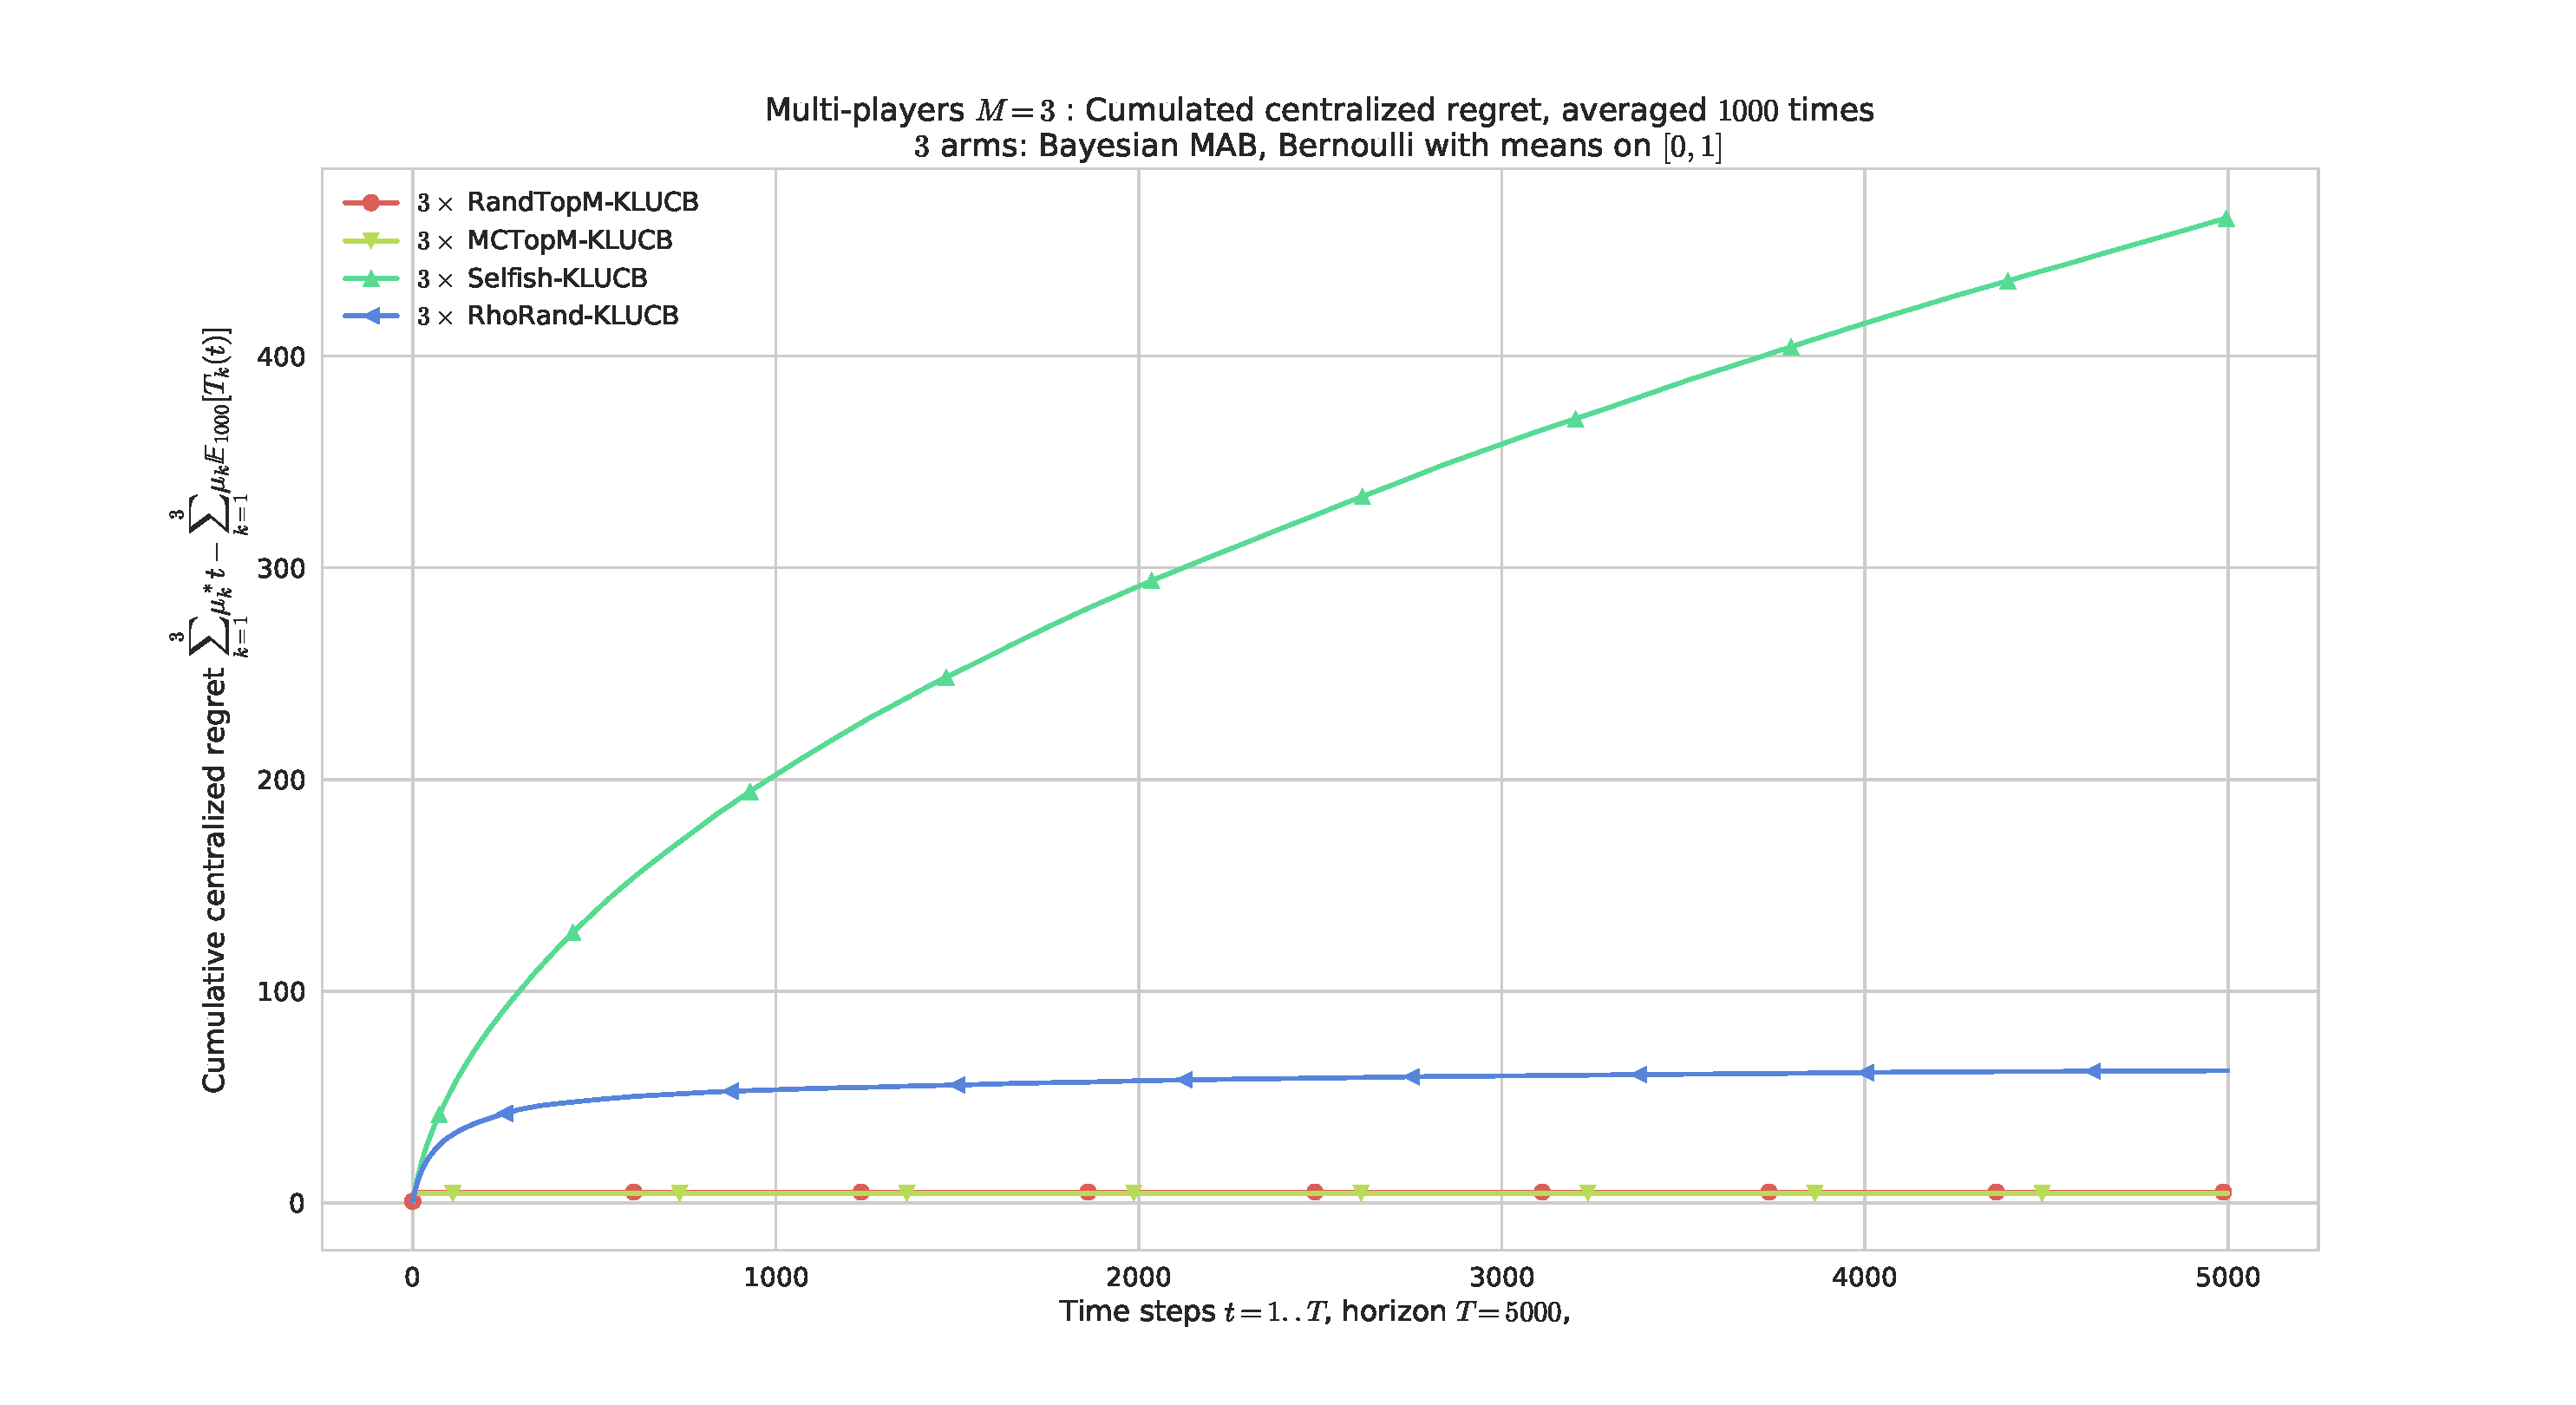
\includegraphics[width=1.00\textwidth]{MP__K3_M3_T5000_N1000__4_algos/all_RegretCentralized____env1-1_4683123079851881812.pdf}
    % \end{subfigure}
    \caption[Second failure case of \Selfish]{Regret, $M=2$ and $M=3$ players, $K=3$ arms, horizon $T=5000$, against $1000$ problems $\boldsymbol{\mu}$ uniformly sampled in $[0,1]^K$. \Selfish{} (top curve in \textcolor{darkgreen}{green}) clearly fails in such setting with small $K$.}
    \label{fig:5:selfish_fail2}
    % \vspace*{-15pt}  % XXX remove if problem
\end{figure}

%
% Regular plots of centralized regrets
%
\begin{figure}[!h]
    \centering
    % \begin{subfigure}[!h]{1.00\textwidth}
        % 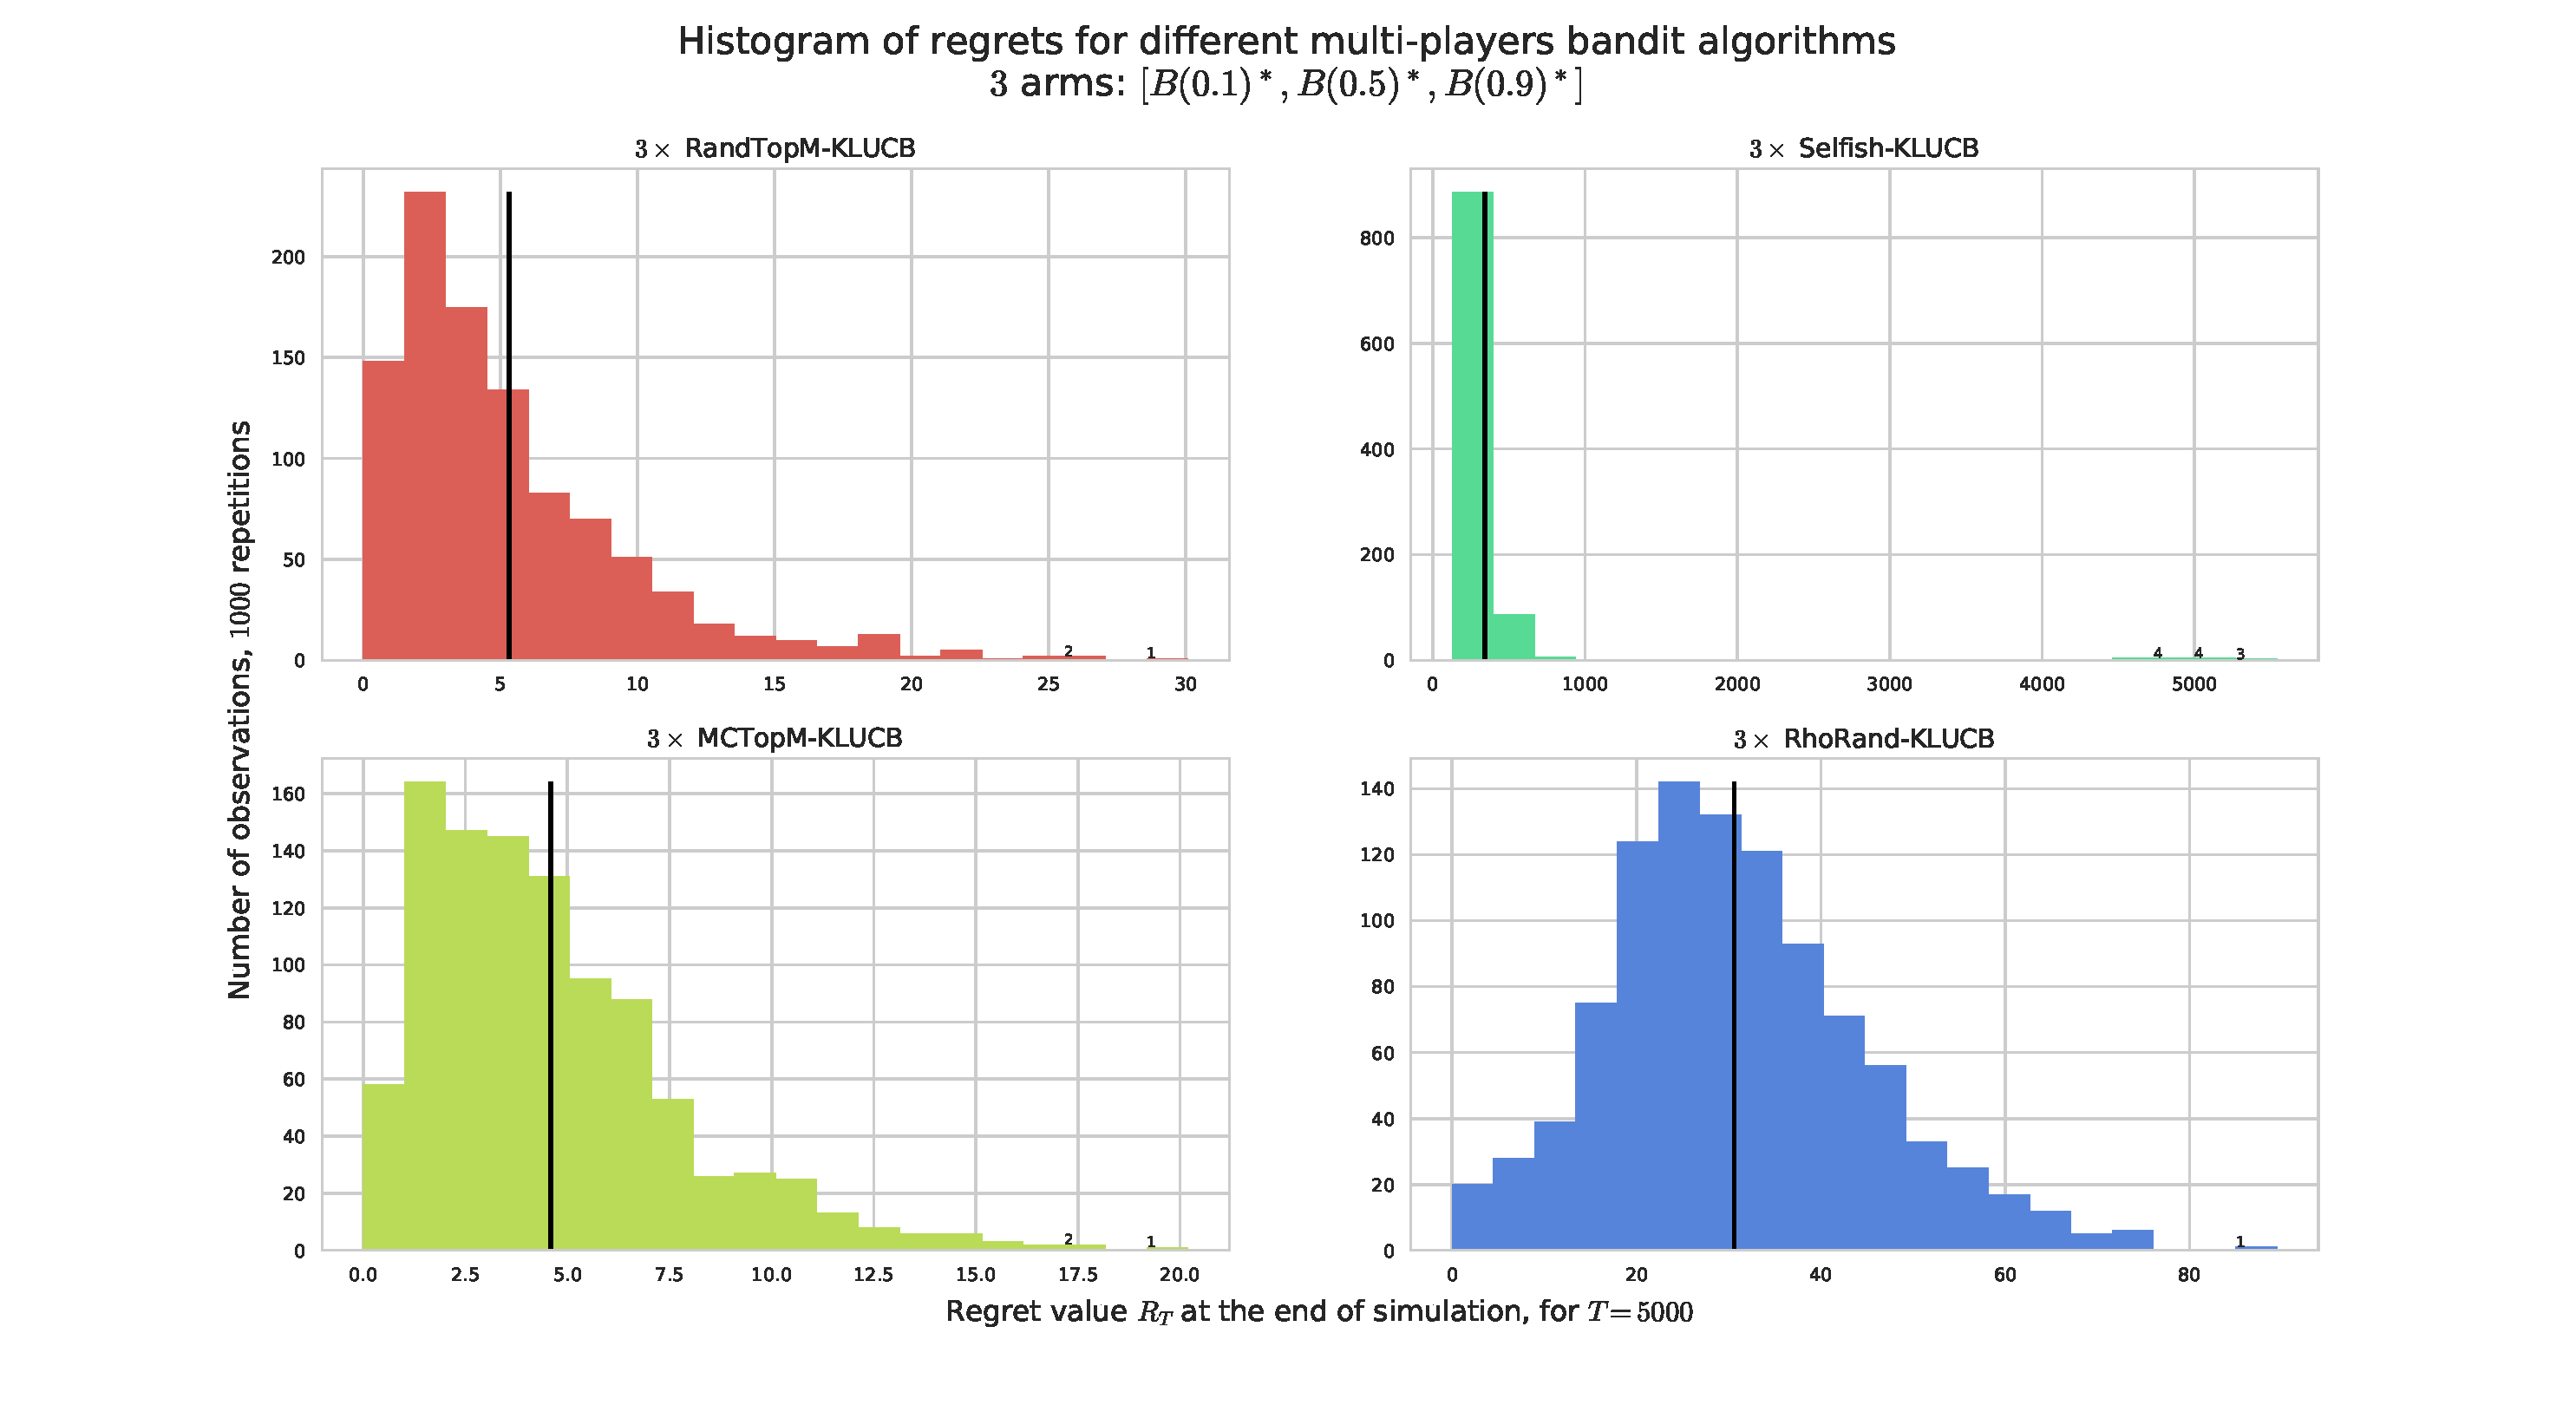
\includegraphics[width=1.00\textwidth]{MP__K3_M3_T5000_N1000__4_algos/all_HistogramsRegret____env1-1_1035303196230283176.pdf}
        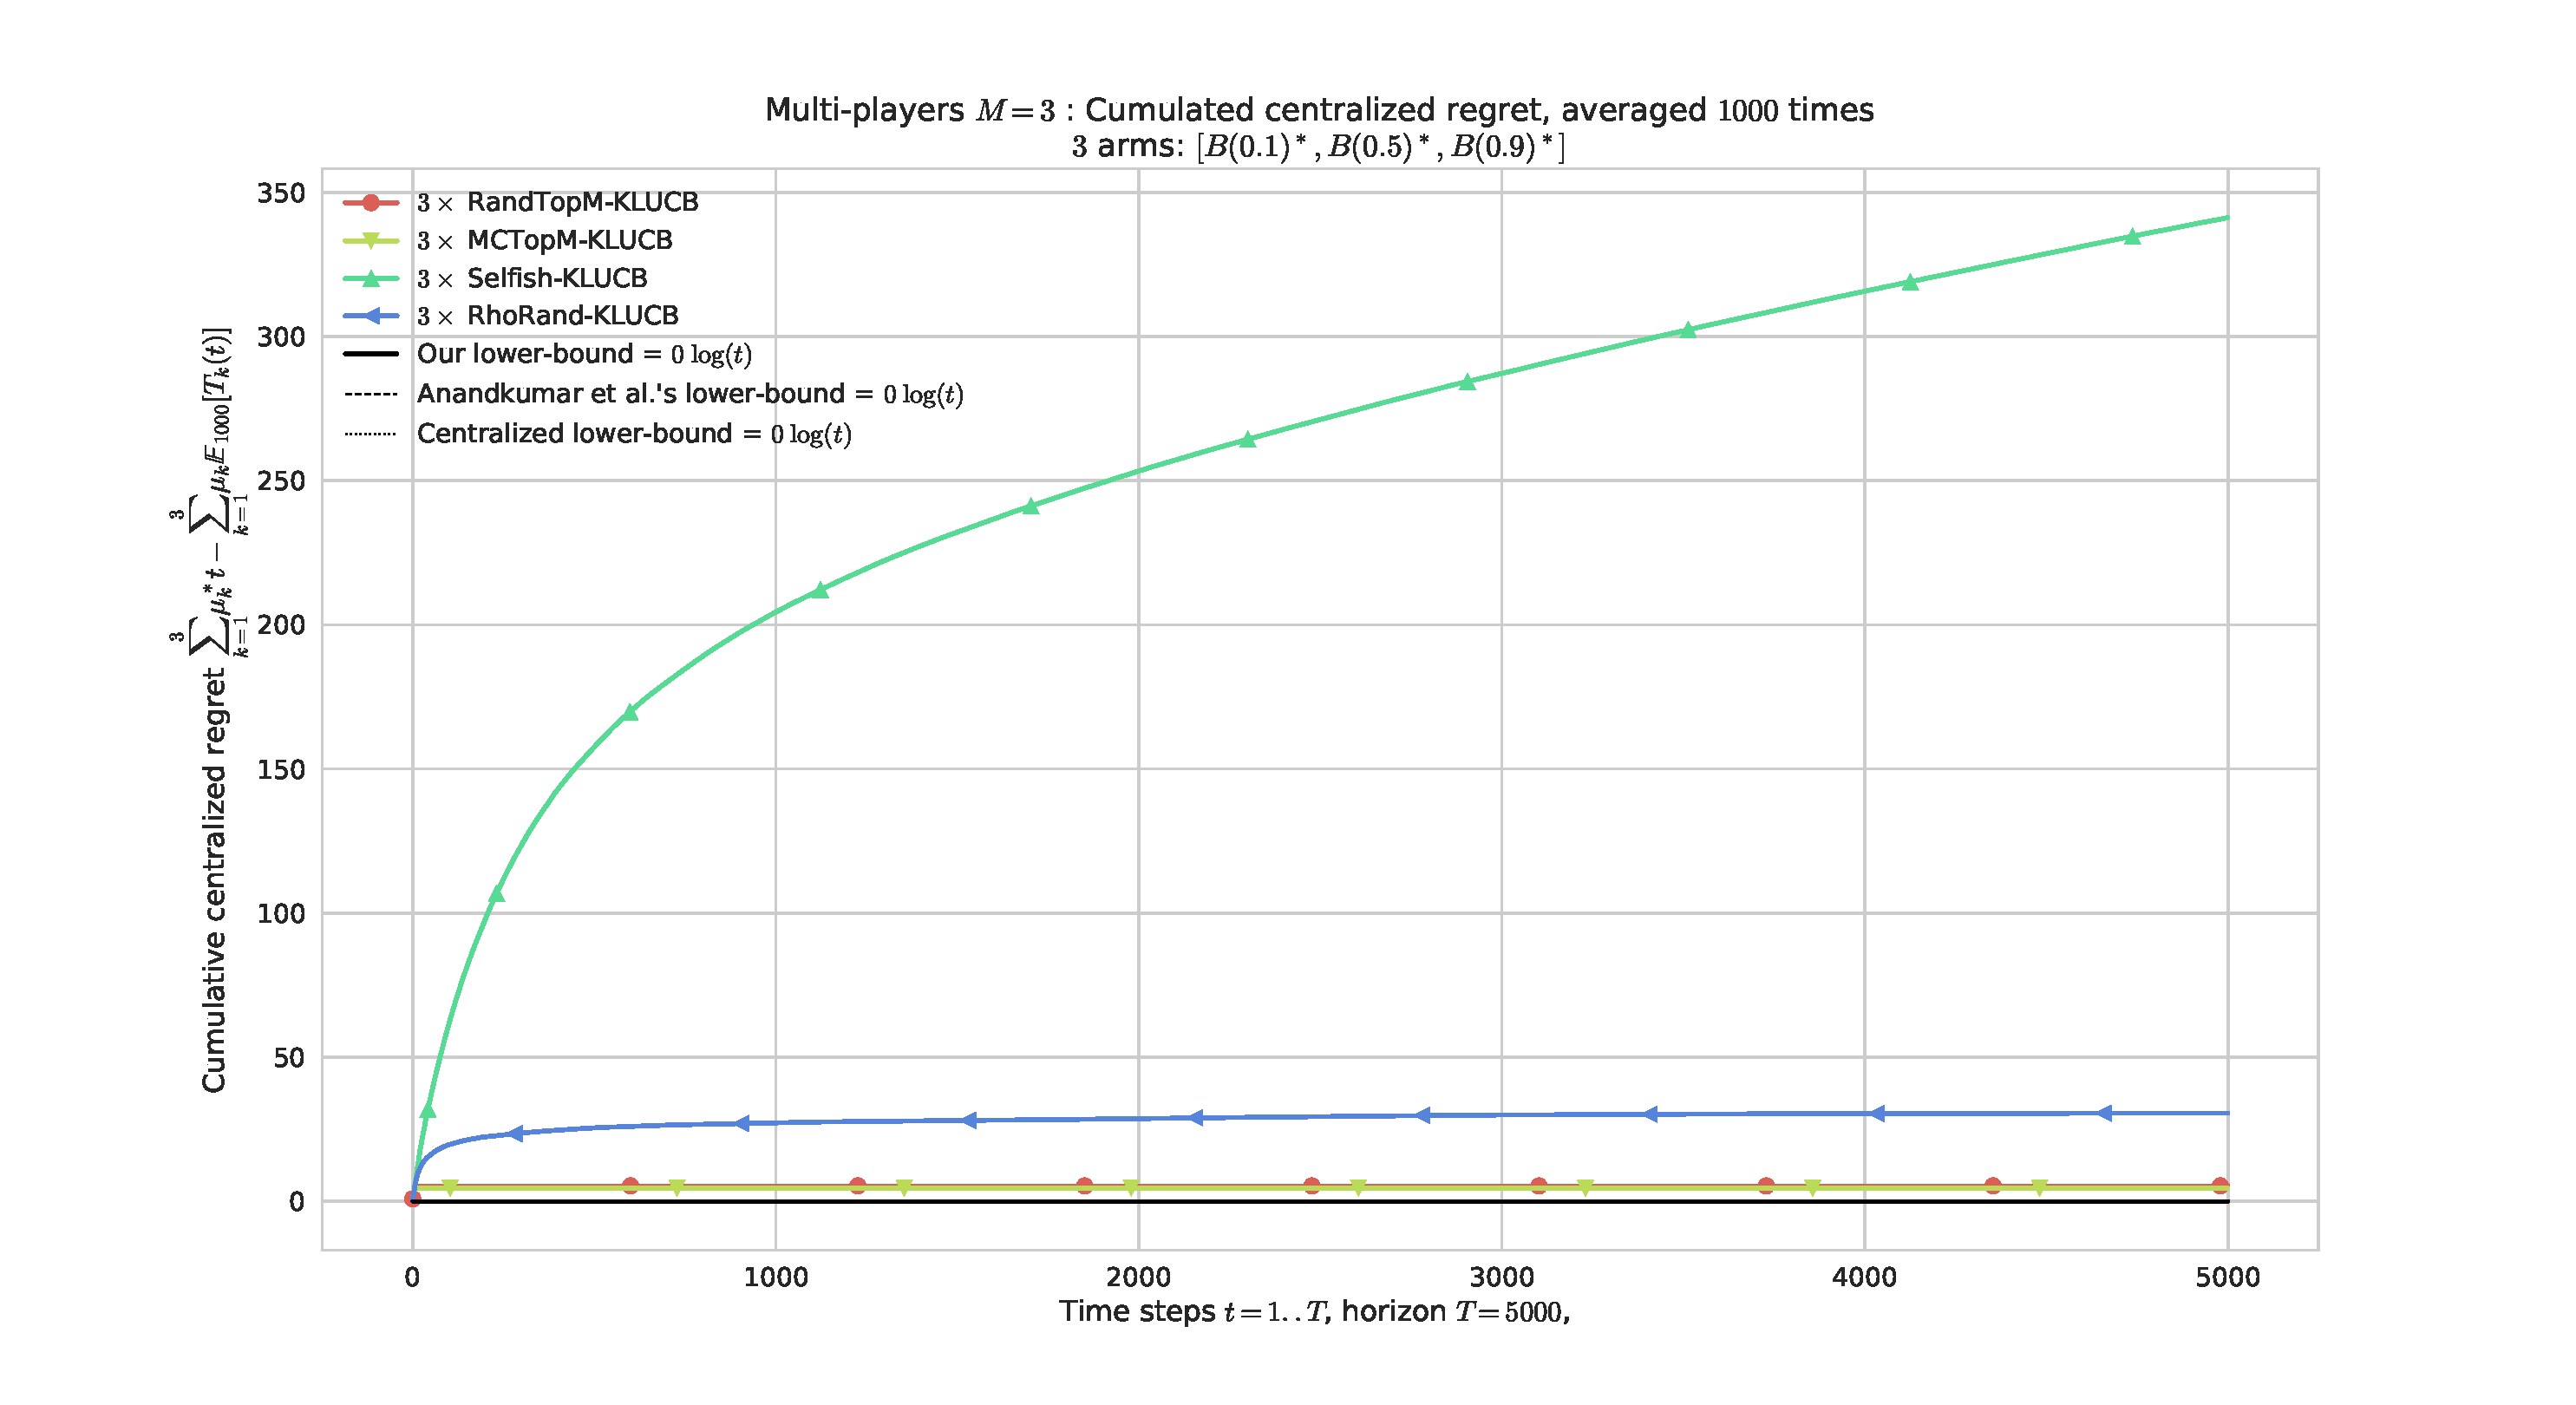
\includegraphics[width=1.00\textwidth]{MP__K3_M3_T5000_N1000__4_algos/all_RegretCentralized____env1-1_1035303196230283176.pdf}
        % 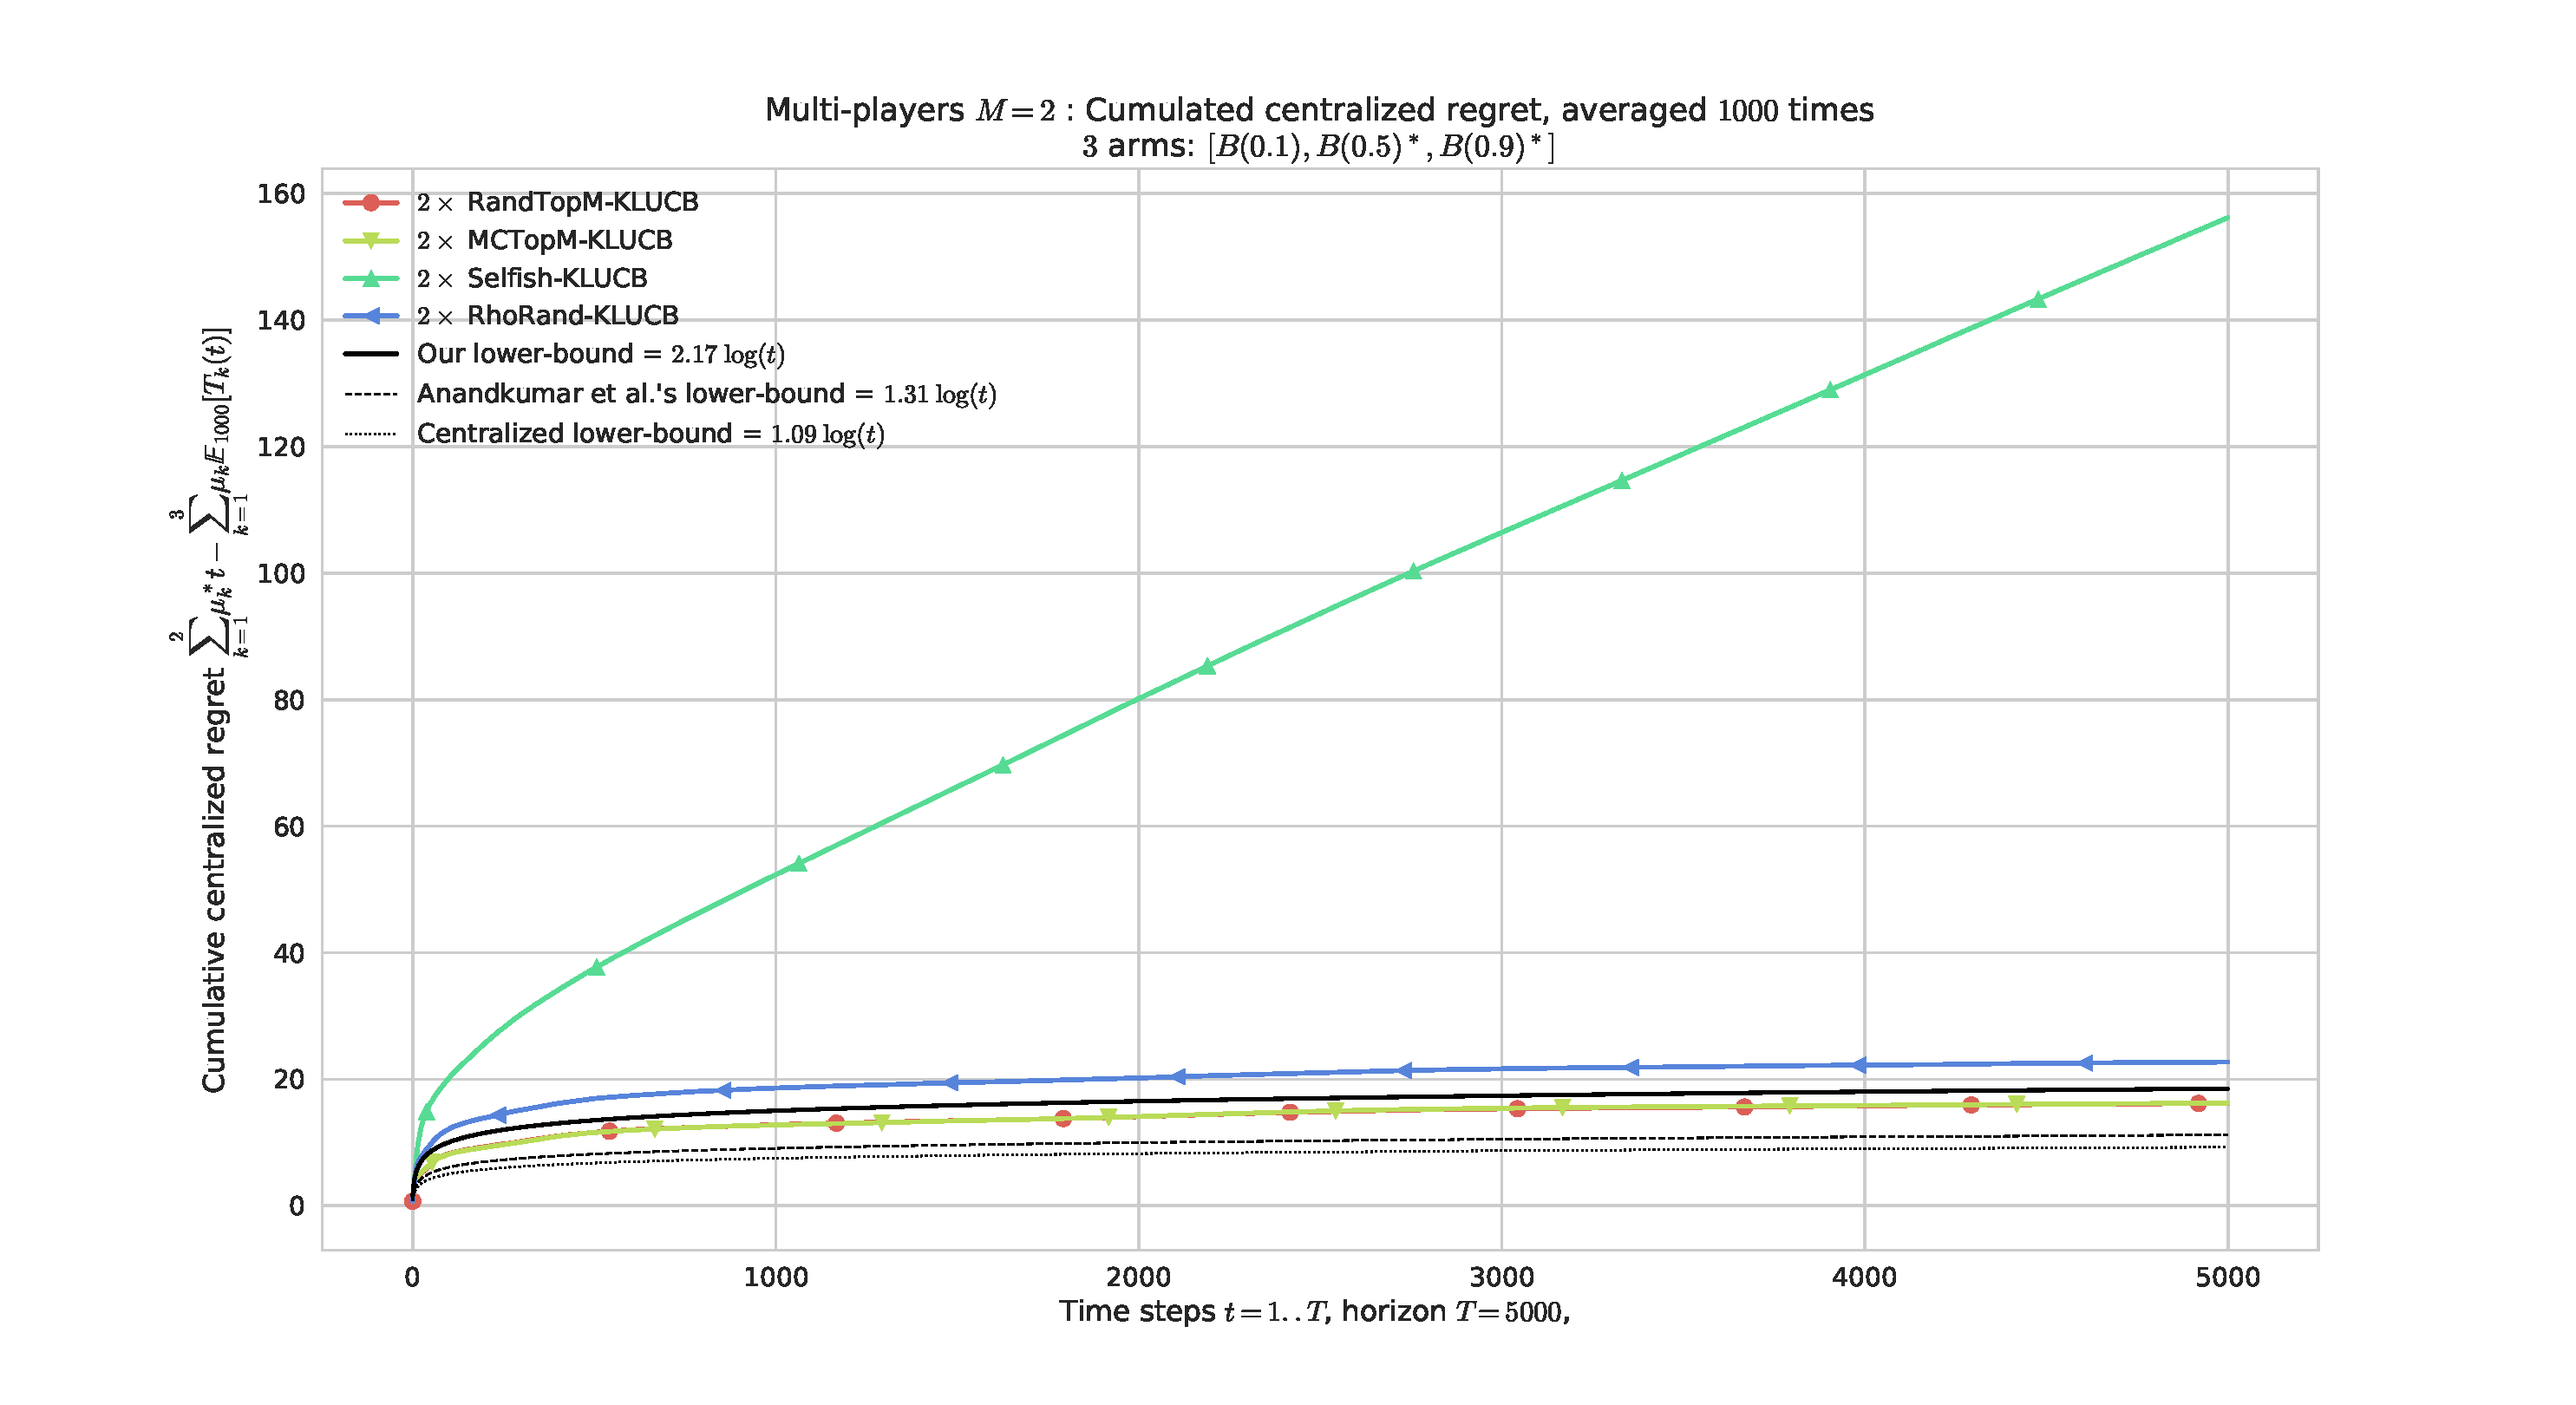
\includegraphics[width=1.00\textwidth]{MP__K3_M2_T5000_N1000__4_algos/all_RegretCentralized____env1-1_5016720151160452442.pdf}
    % \end{subfigure}
    ~
    % \begin{subfigure}[!h]{1.00\textwidth}
        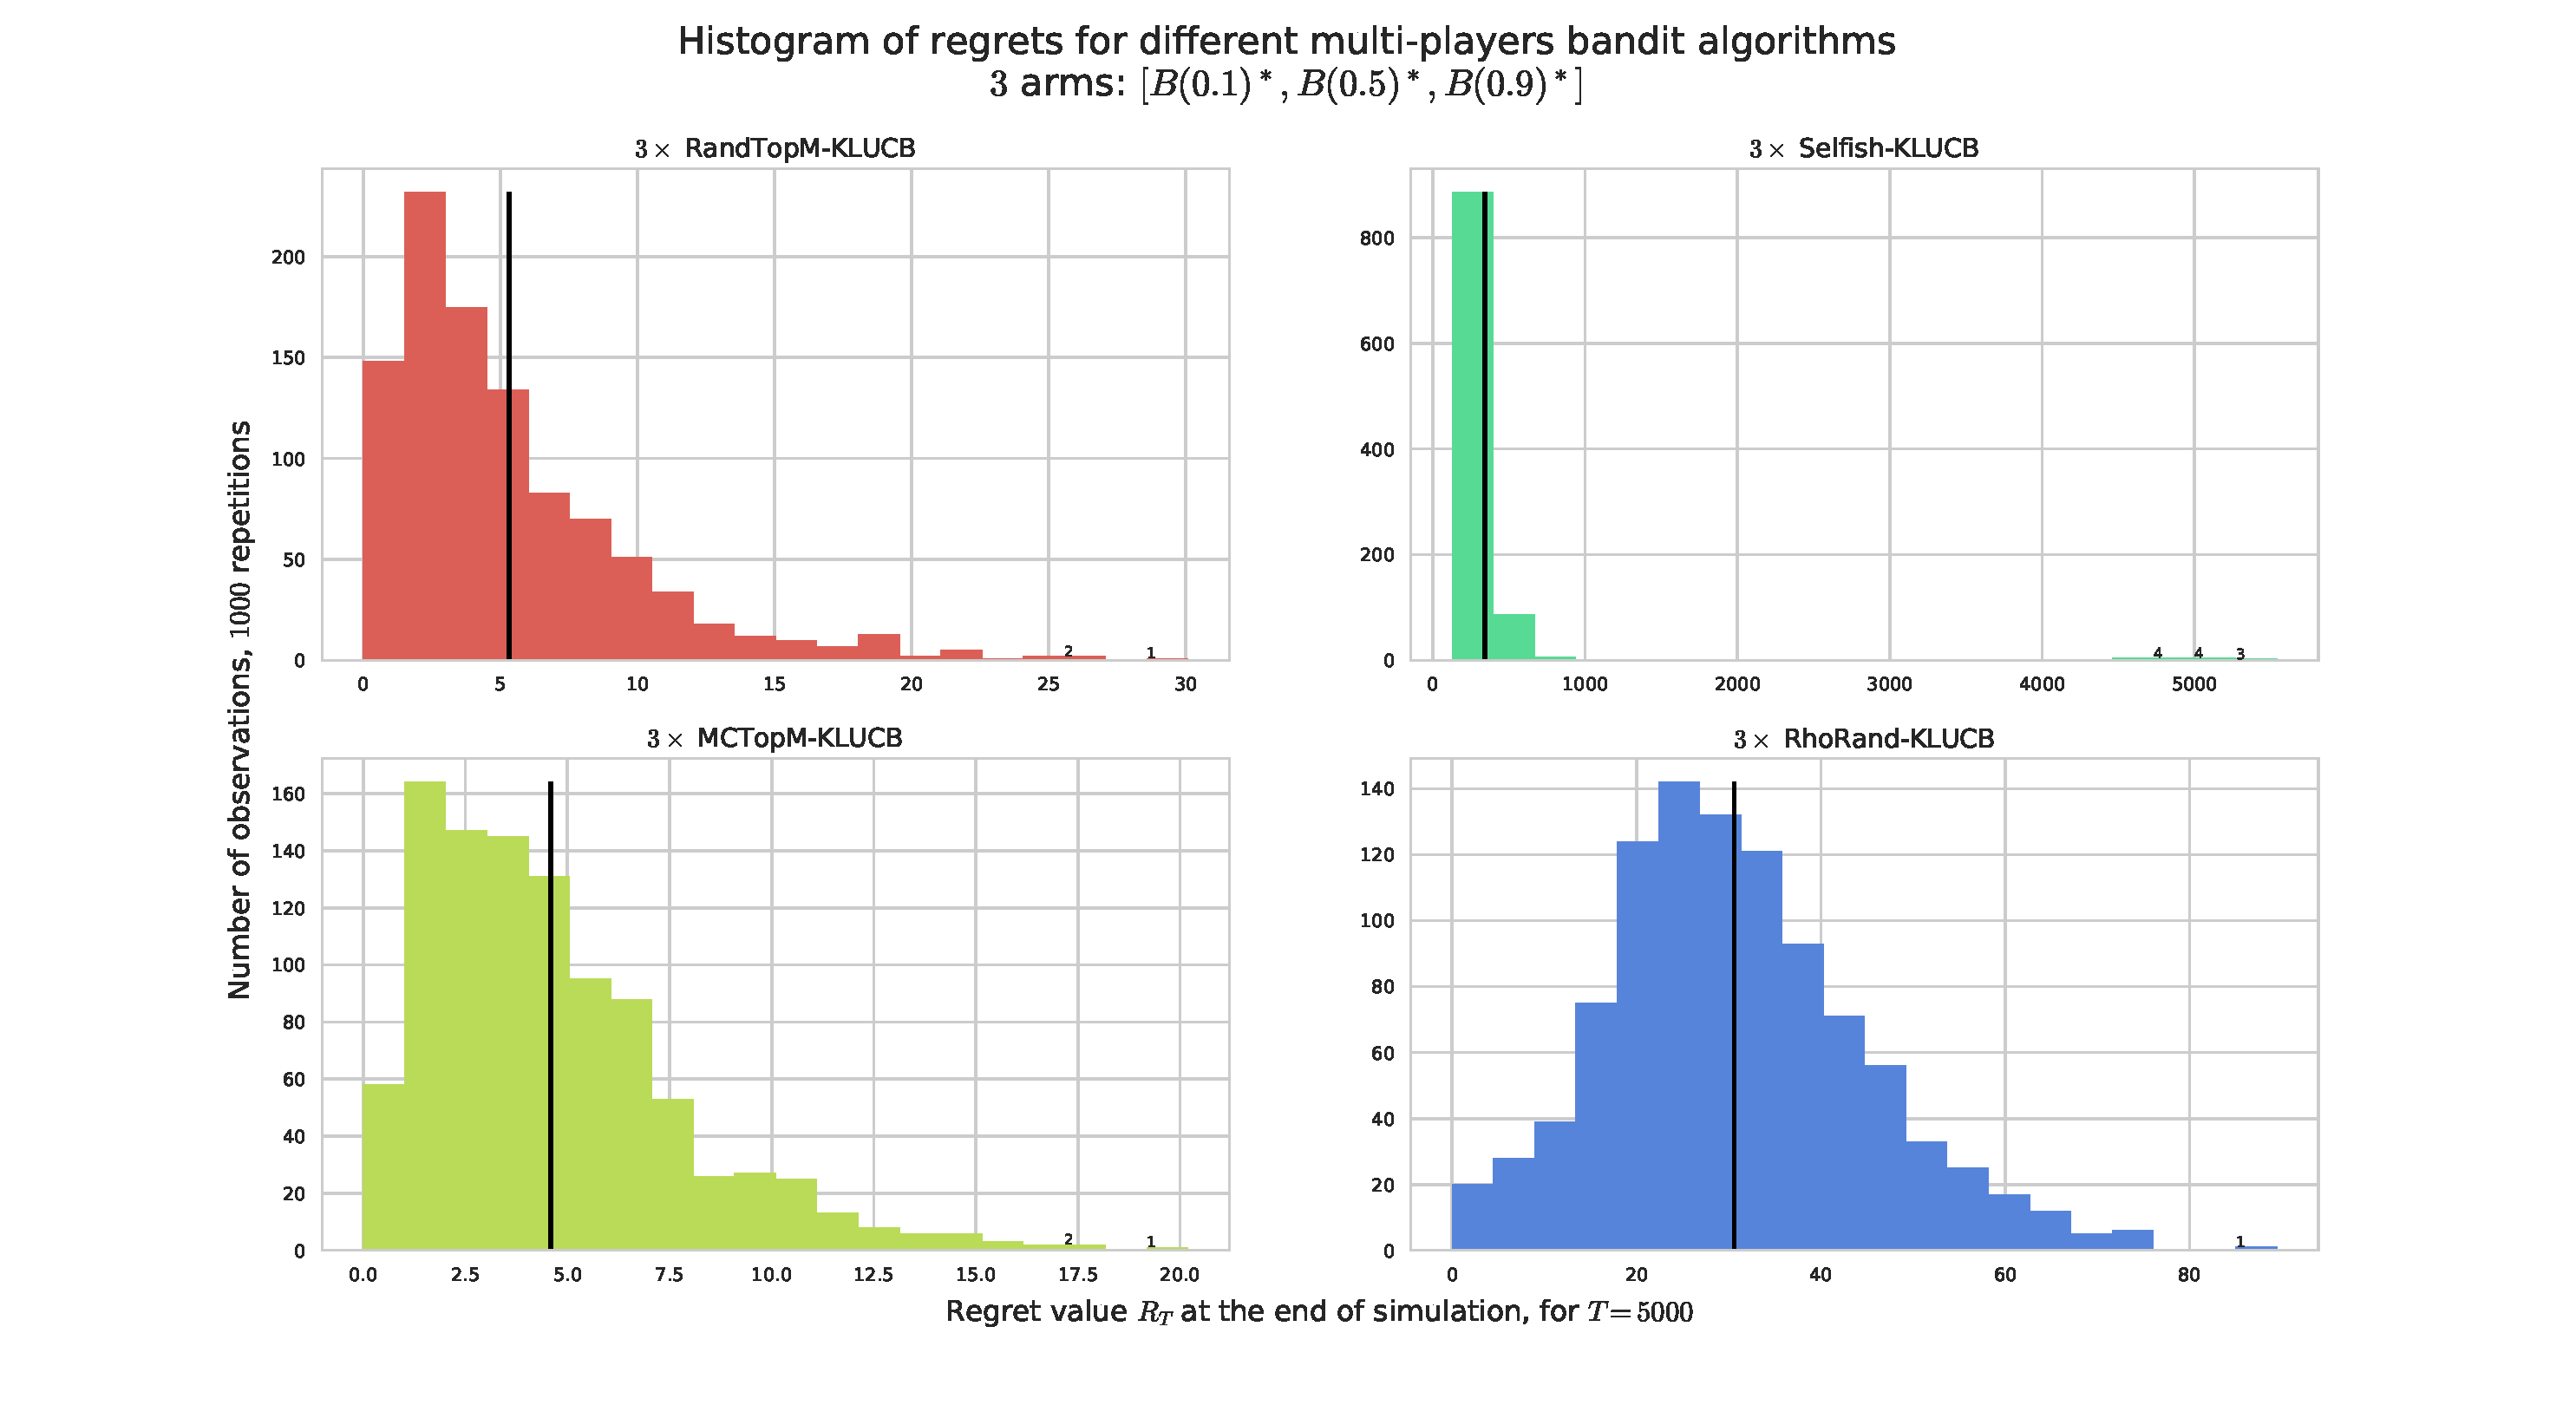
\includegraphics[width=1.00\textwidth]{MP__K3_M3_T5000_N1000__4_algos/all_HistogramsRegret____env1-1_1035303196230283176.pdf}
    % \end{subfigure}
    \caption[Third failure case of \Selfish]{Regret for $M=3$ players, $K=3$ arms, horizon $T=5000$, $1000$ repetitions and $\boldsymbol{\mu} = [0.1, 0.5, 0.9]$. Axis $x$ is for regret (different scale for each), and the top \textcolor{darkgreen}{green} curve for \Selfish{} shows a small probability of having a linear regret ($11$ cases of $R_T \geq T$, out of $1000$). The regret for the three other algorithms is very small for this problem, and even appears constant.}
    \label{fig:5:selfish_fail3}
    % \vspace*{-15pt}  % XXX remove if problem
\end{figure}

%
% Regular plots of centralized regrets
%

\begin{figure}[!h]
    \centering
    % \begin{subfigure}[!h]{1.00\textwidth}
        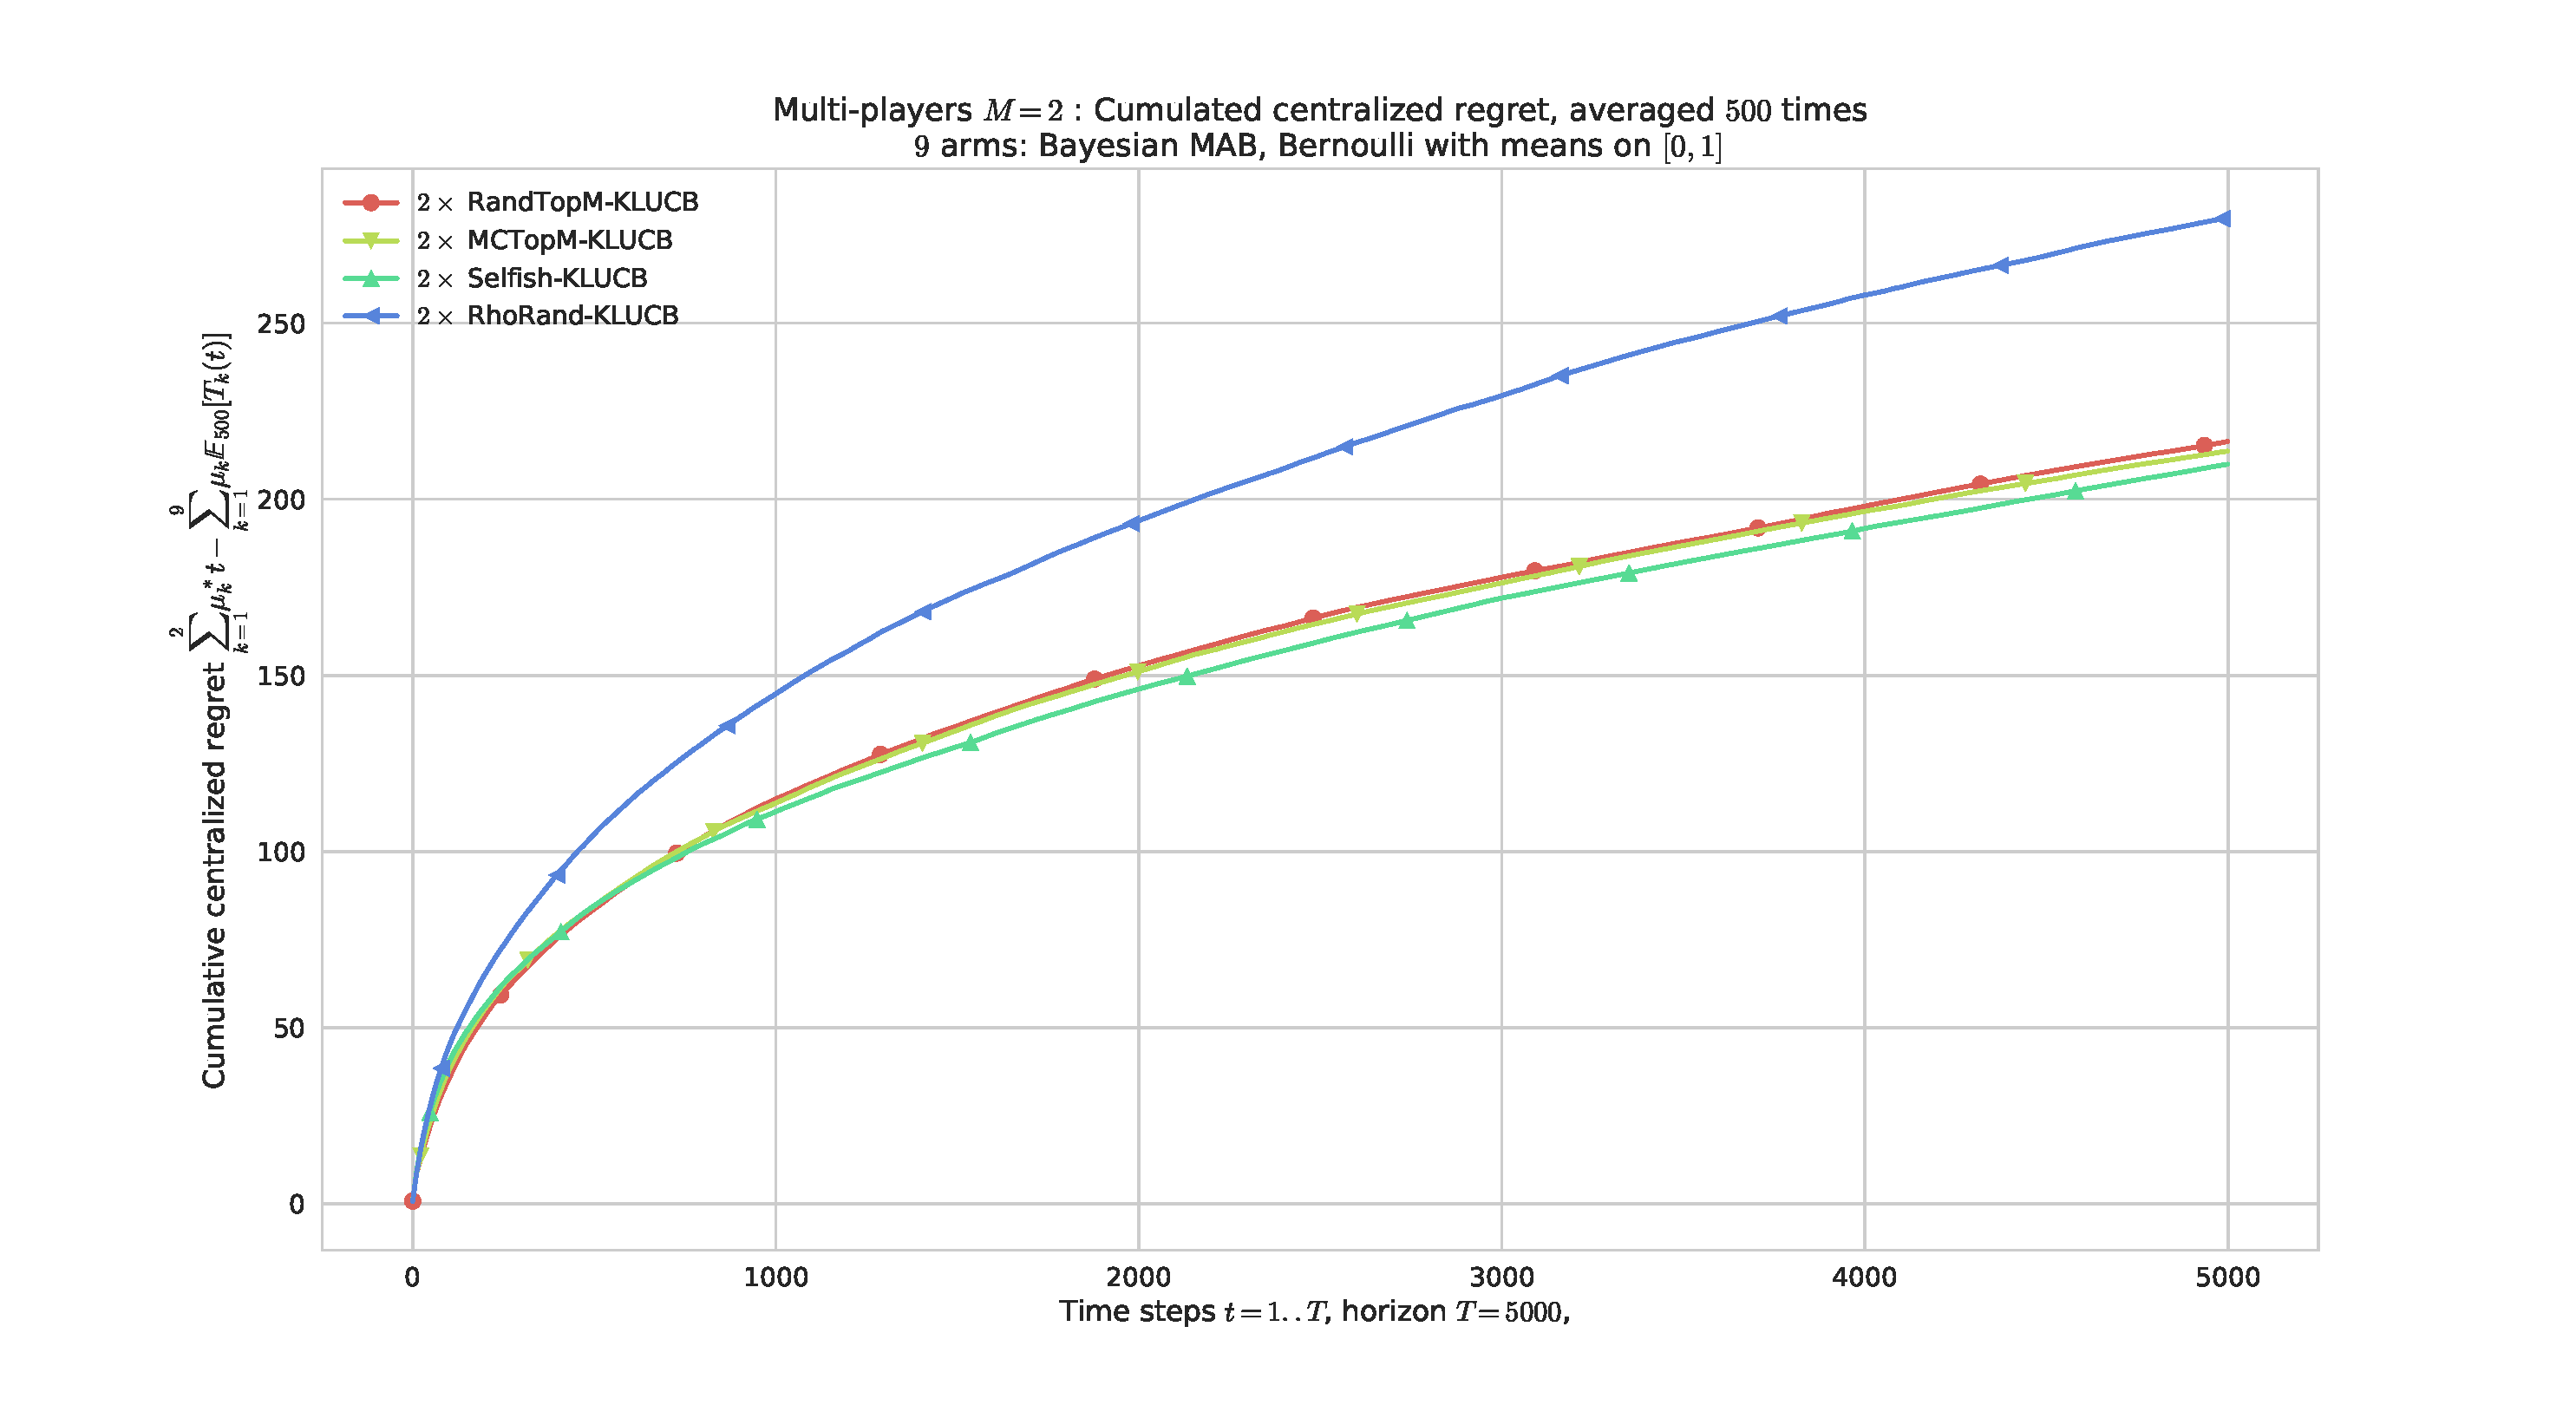
\includegraphics[width=1.00\textwidth]{MP__K9_M2_T5000_N500__4_algos/all_RegretCentralized____env1-1_3251433209347345969.pdf}
    % \end{subfigure}
    % ~
    % \begin{subfigure}[!h]{1.00\textwidth}
        % 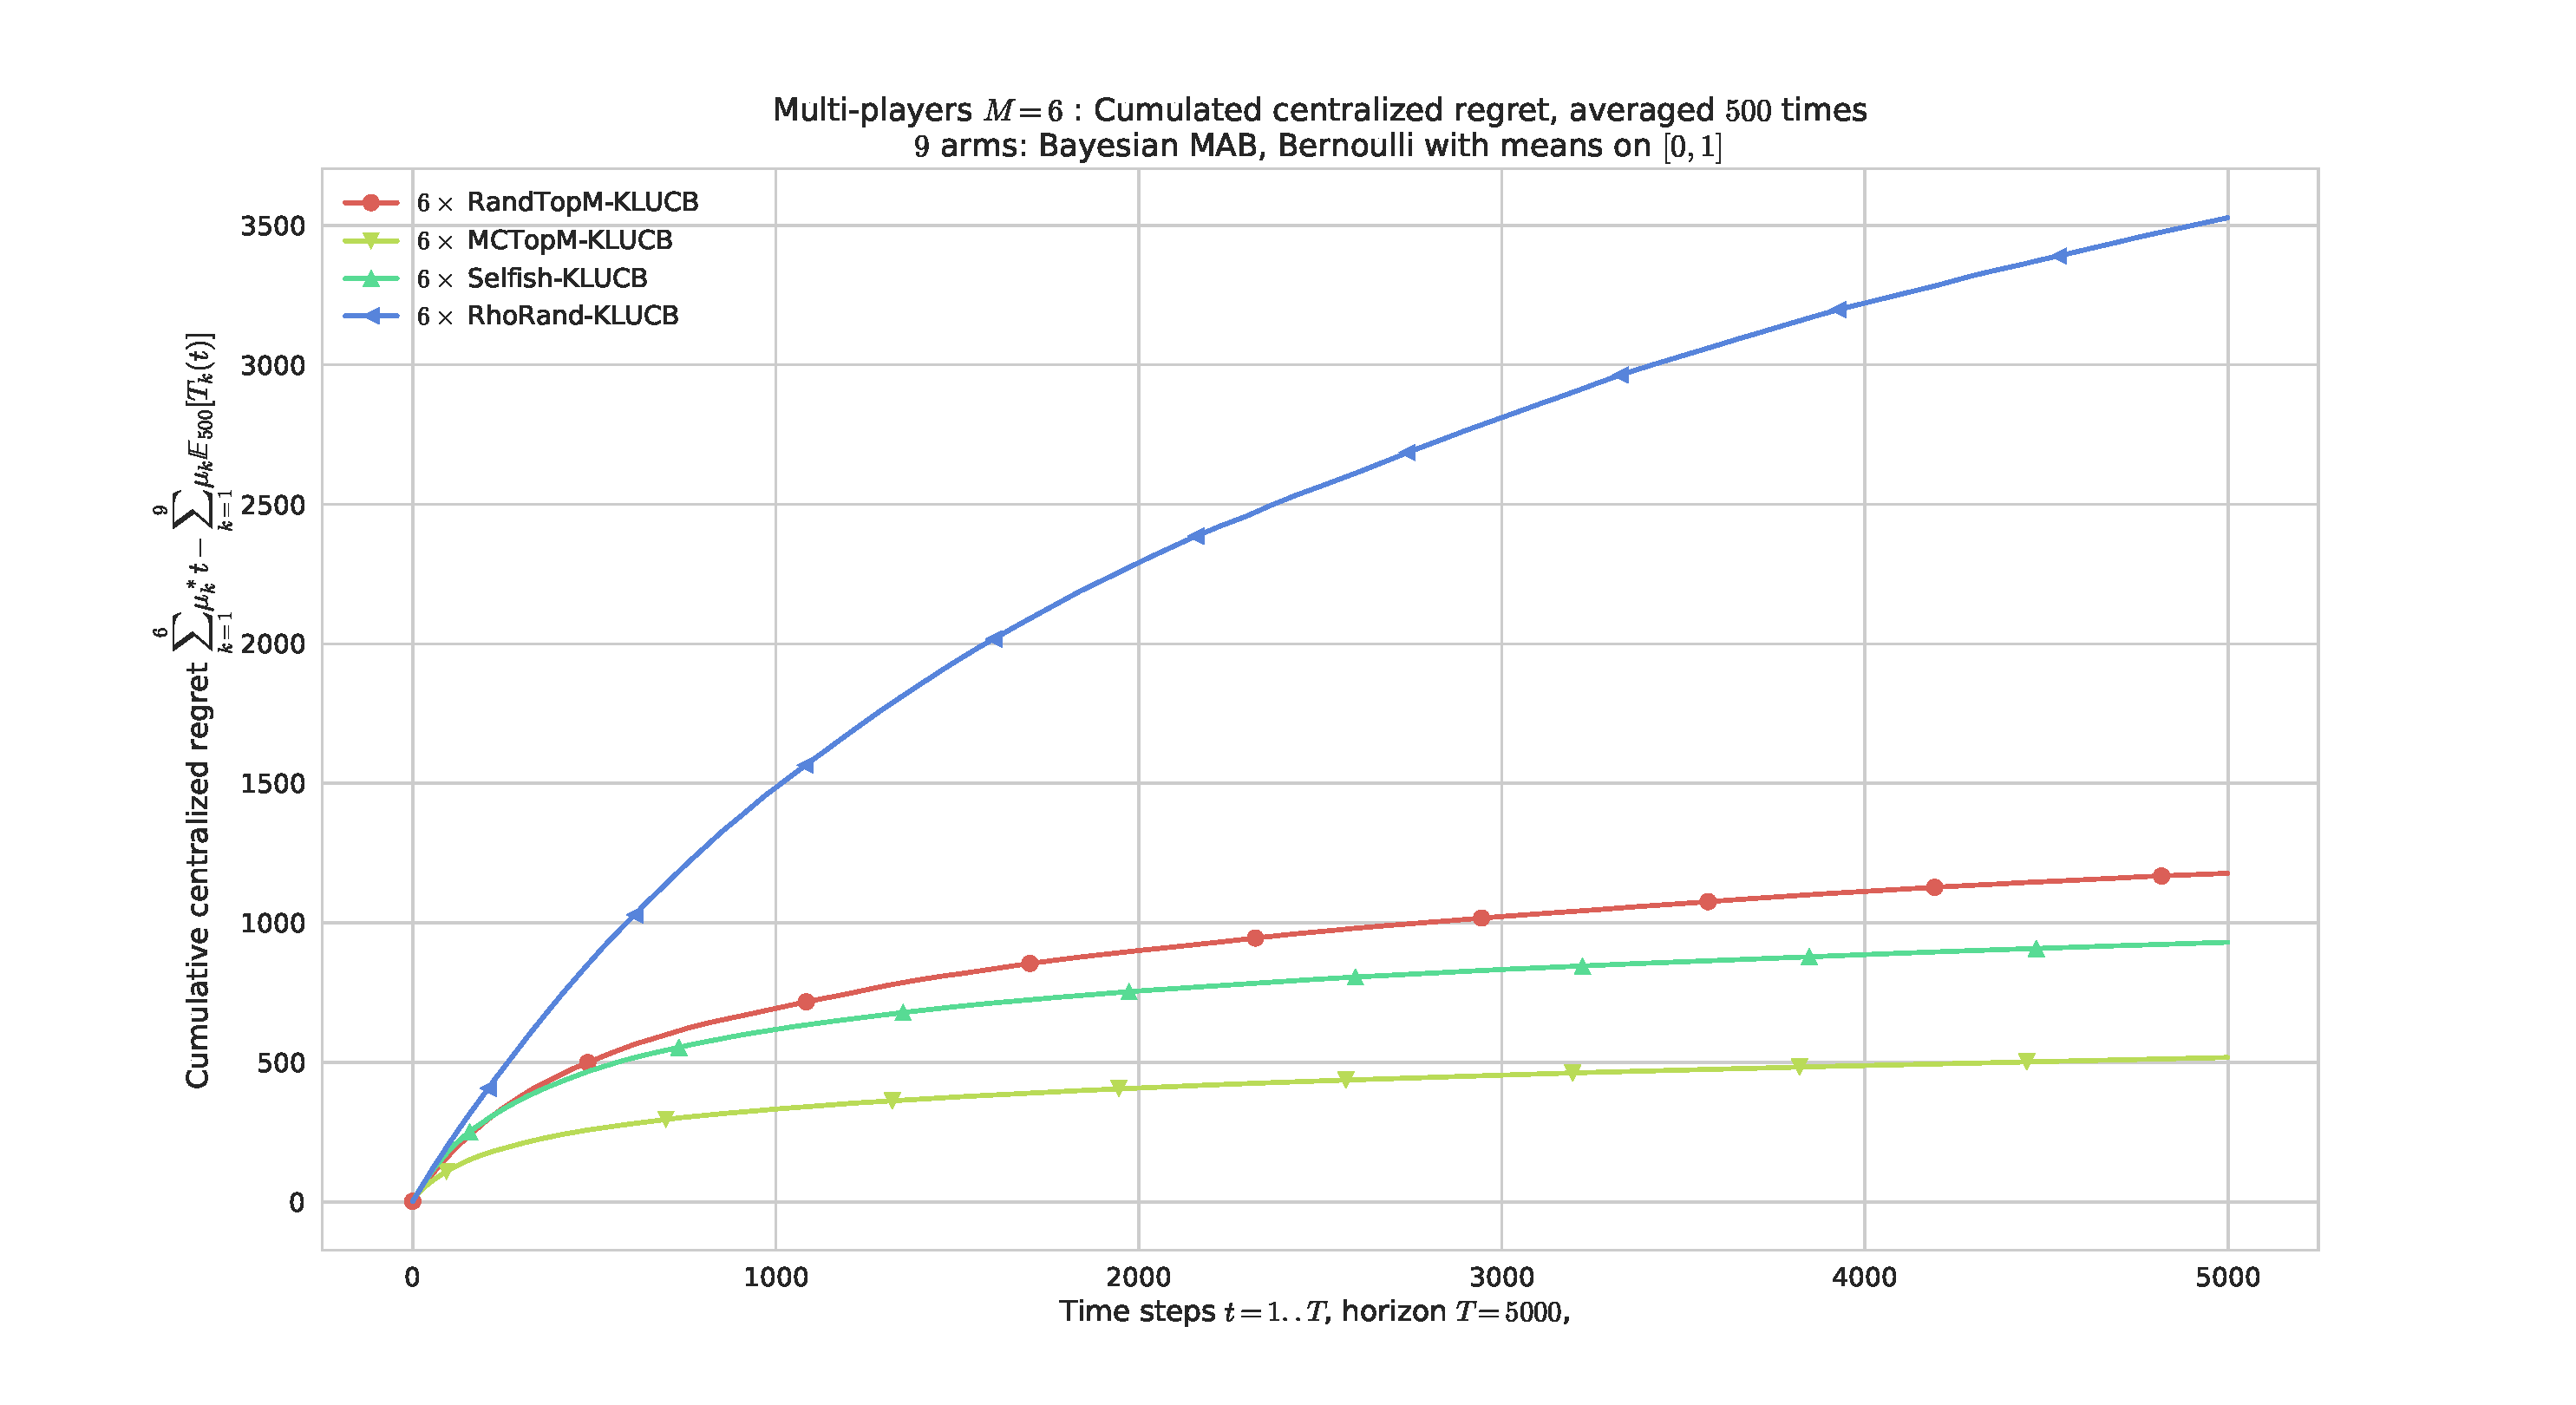
\includegraphics[width=1.00\textwidth]{MP__K9_M6_T5000_N500__4_algos/all_RegretCentralized____env1-1_8318947830261751207.pdf}
        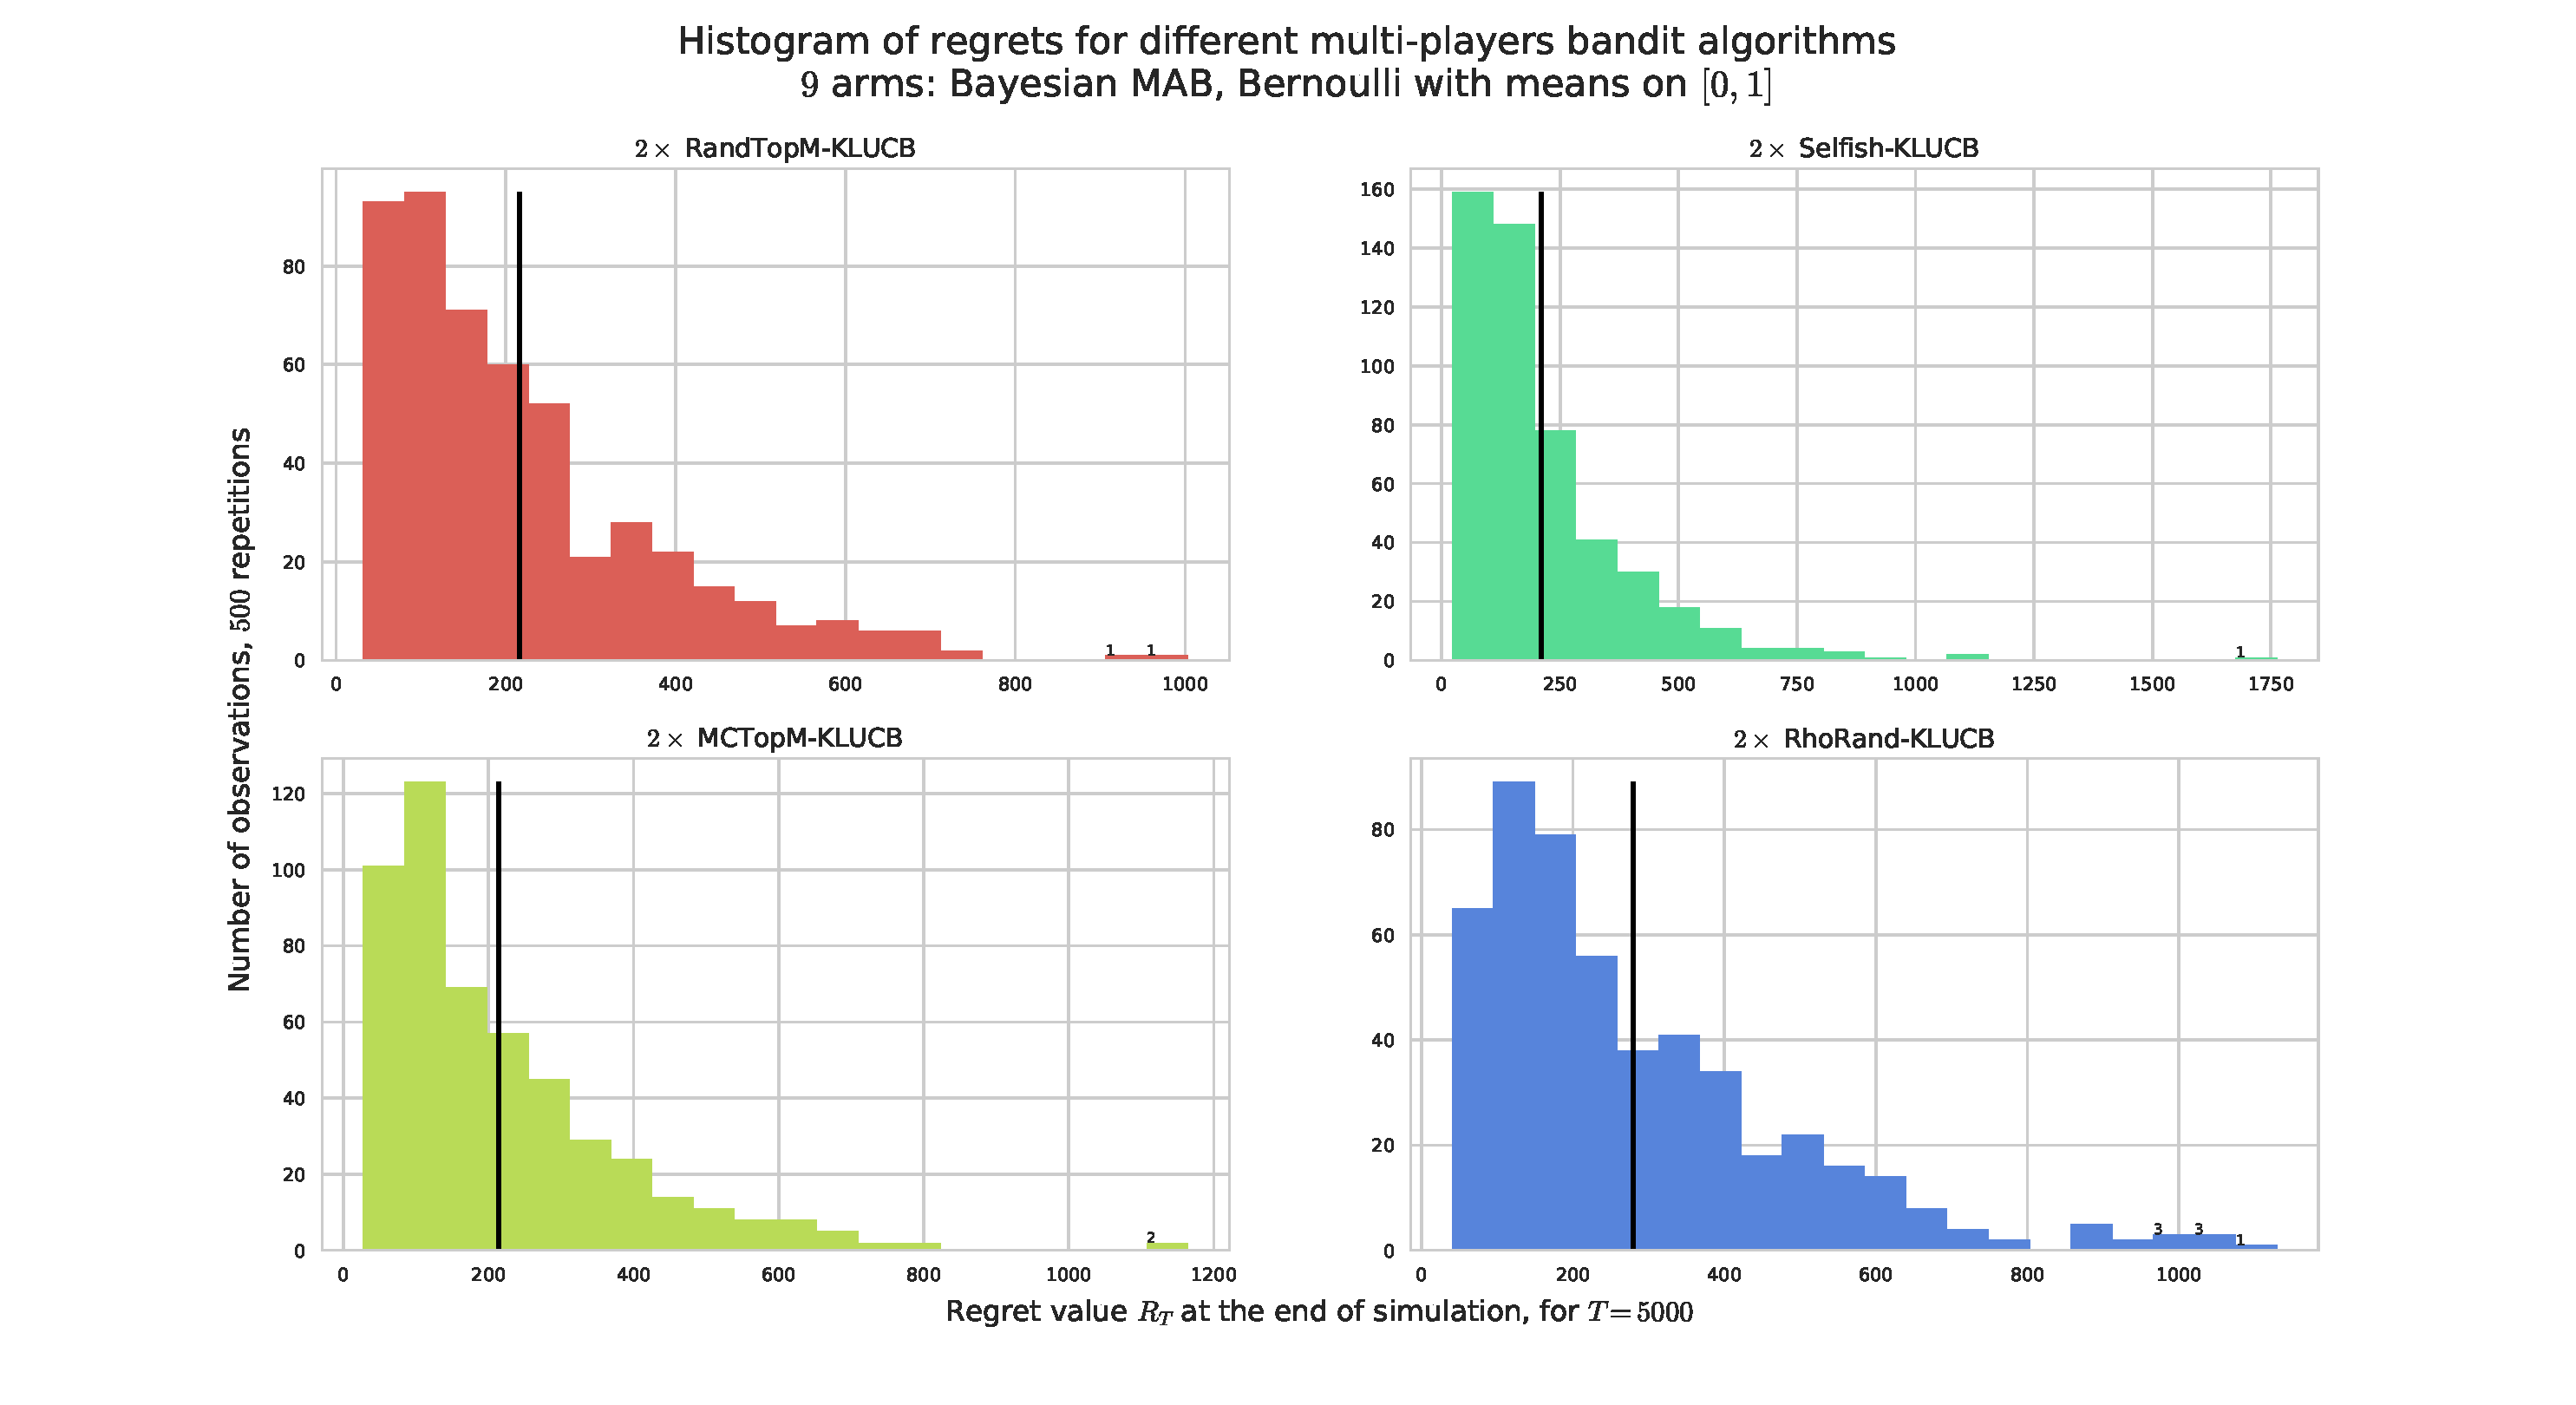
\includegraphics[width=1.00\textwidth]{MP__K9_M2_T5000_N500__4_algos/all_HistogramsRegret____env1-1_3251433209347345969.pdf}
    % \end{subfigure}
    \caption[Regret for $M=2$ players, $K=9$ arms, horizon $T=5000$, against $500$ problems $\boldsymbol{\mu}$ uniformly sampled]{Regret for $M=2$ players, $K=9$ arms, horizon $T=5000$, against $500$ problems $\boldsymbol{\mu}$ uniformly sampled in $[0,1]^K$. \rhoRand{} (top \textcolor{blue}{blue}) is outperformed by the other algorithms (and the gain increases when $M$ increases), which all perform similarly in such configurations. Note that the (small) tail of the histograms come from complicated problems $\boldsymbol{\mu}$ and not failure cases.}
    \label{fig:5:MP__K9_M2_T5000_N500__4_algos__all_RegretCentralized__BayesianProblems}
    % \vspace*{-15pt}  % XXX remove if problem
\end{figure}


\begin{figure}[!h]
    \centering
    % \begin{subfigure}[!h]{1.00\textwidth}
        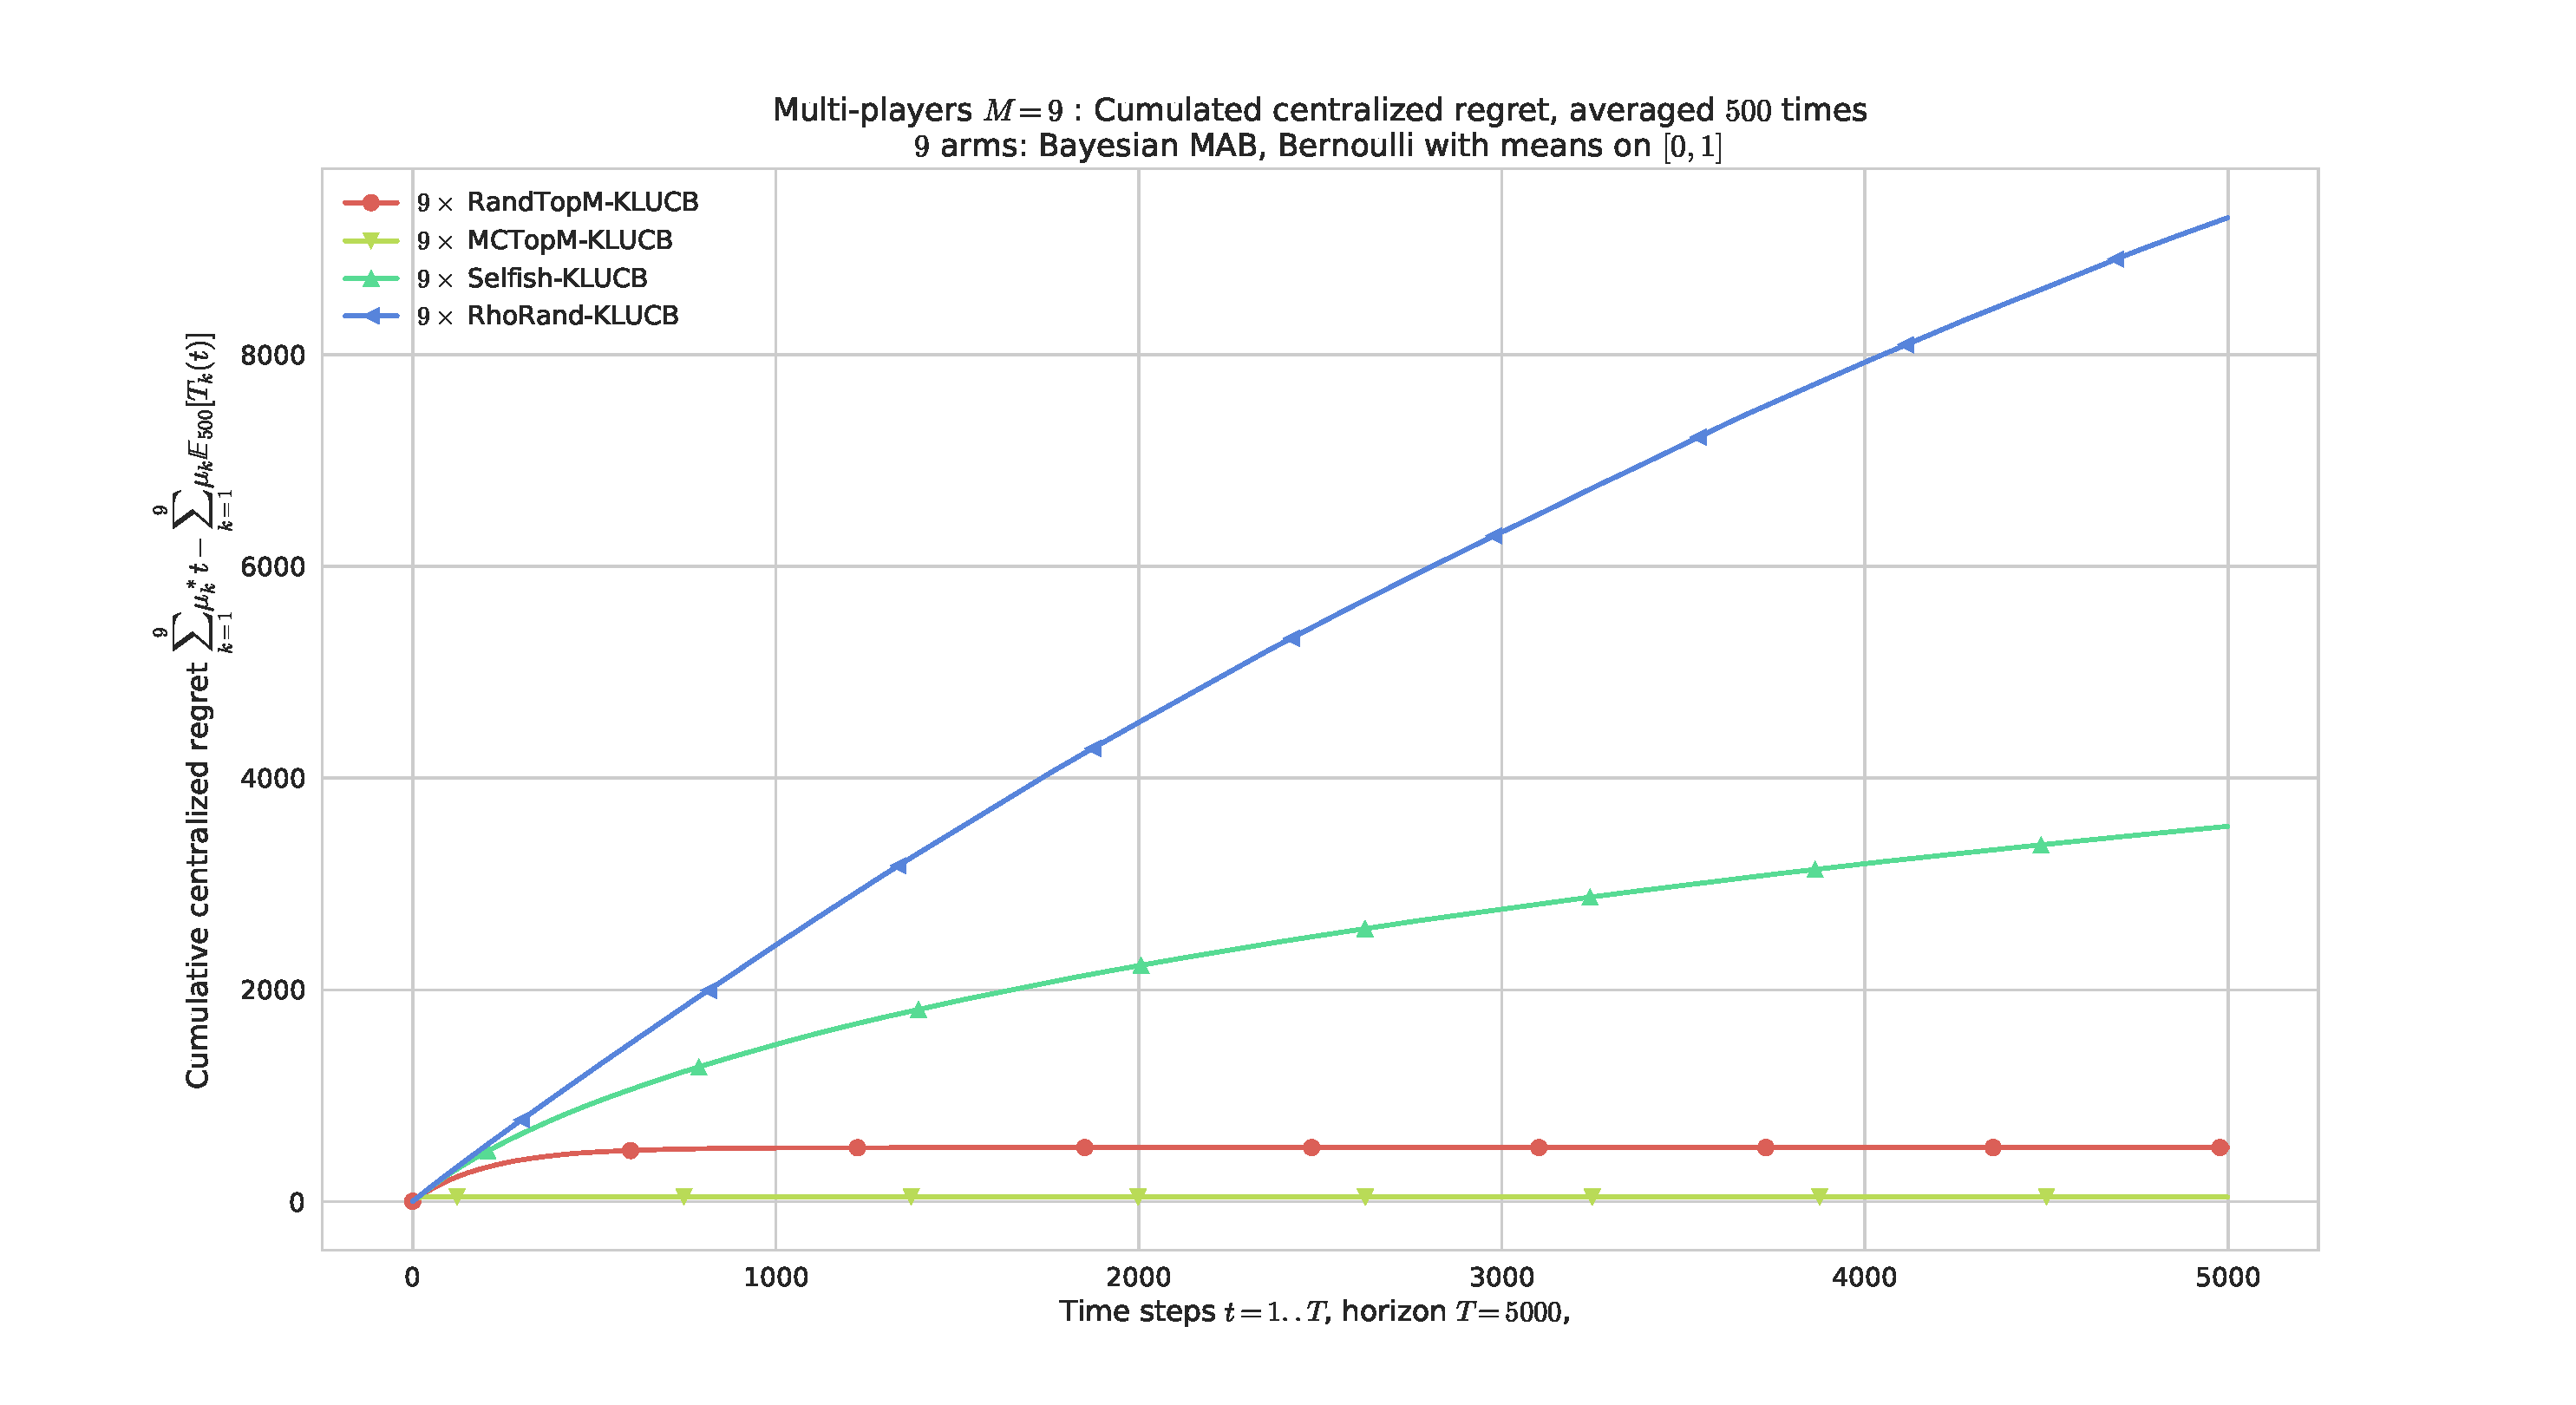
\includegraphics[width=1.00\textwidth]{MP__K9_M9_T5000_N500__4_algos/all_RegretCentralized____env1-1_3892966382091165662.pdf}
    % \end{subfigure}
    % ~
    % \begin{subfigure}[!h]{1.00\textwidth}
        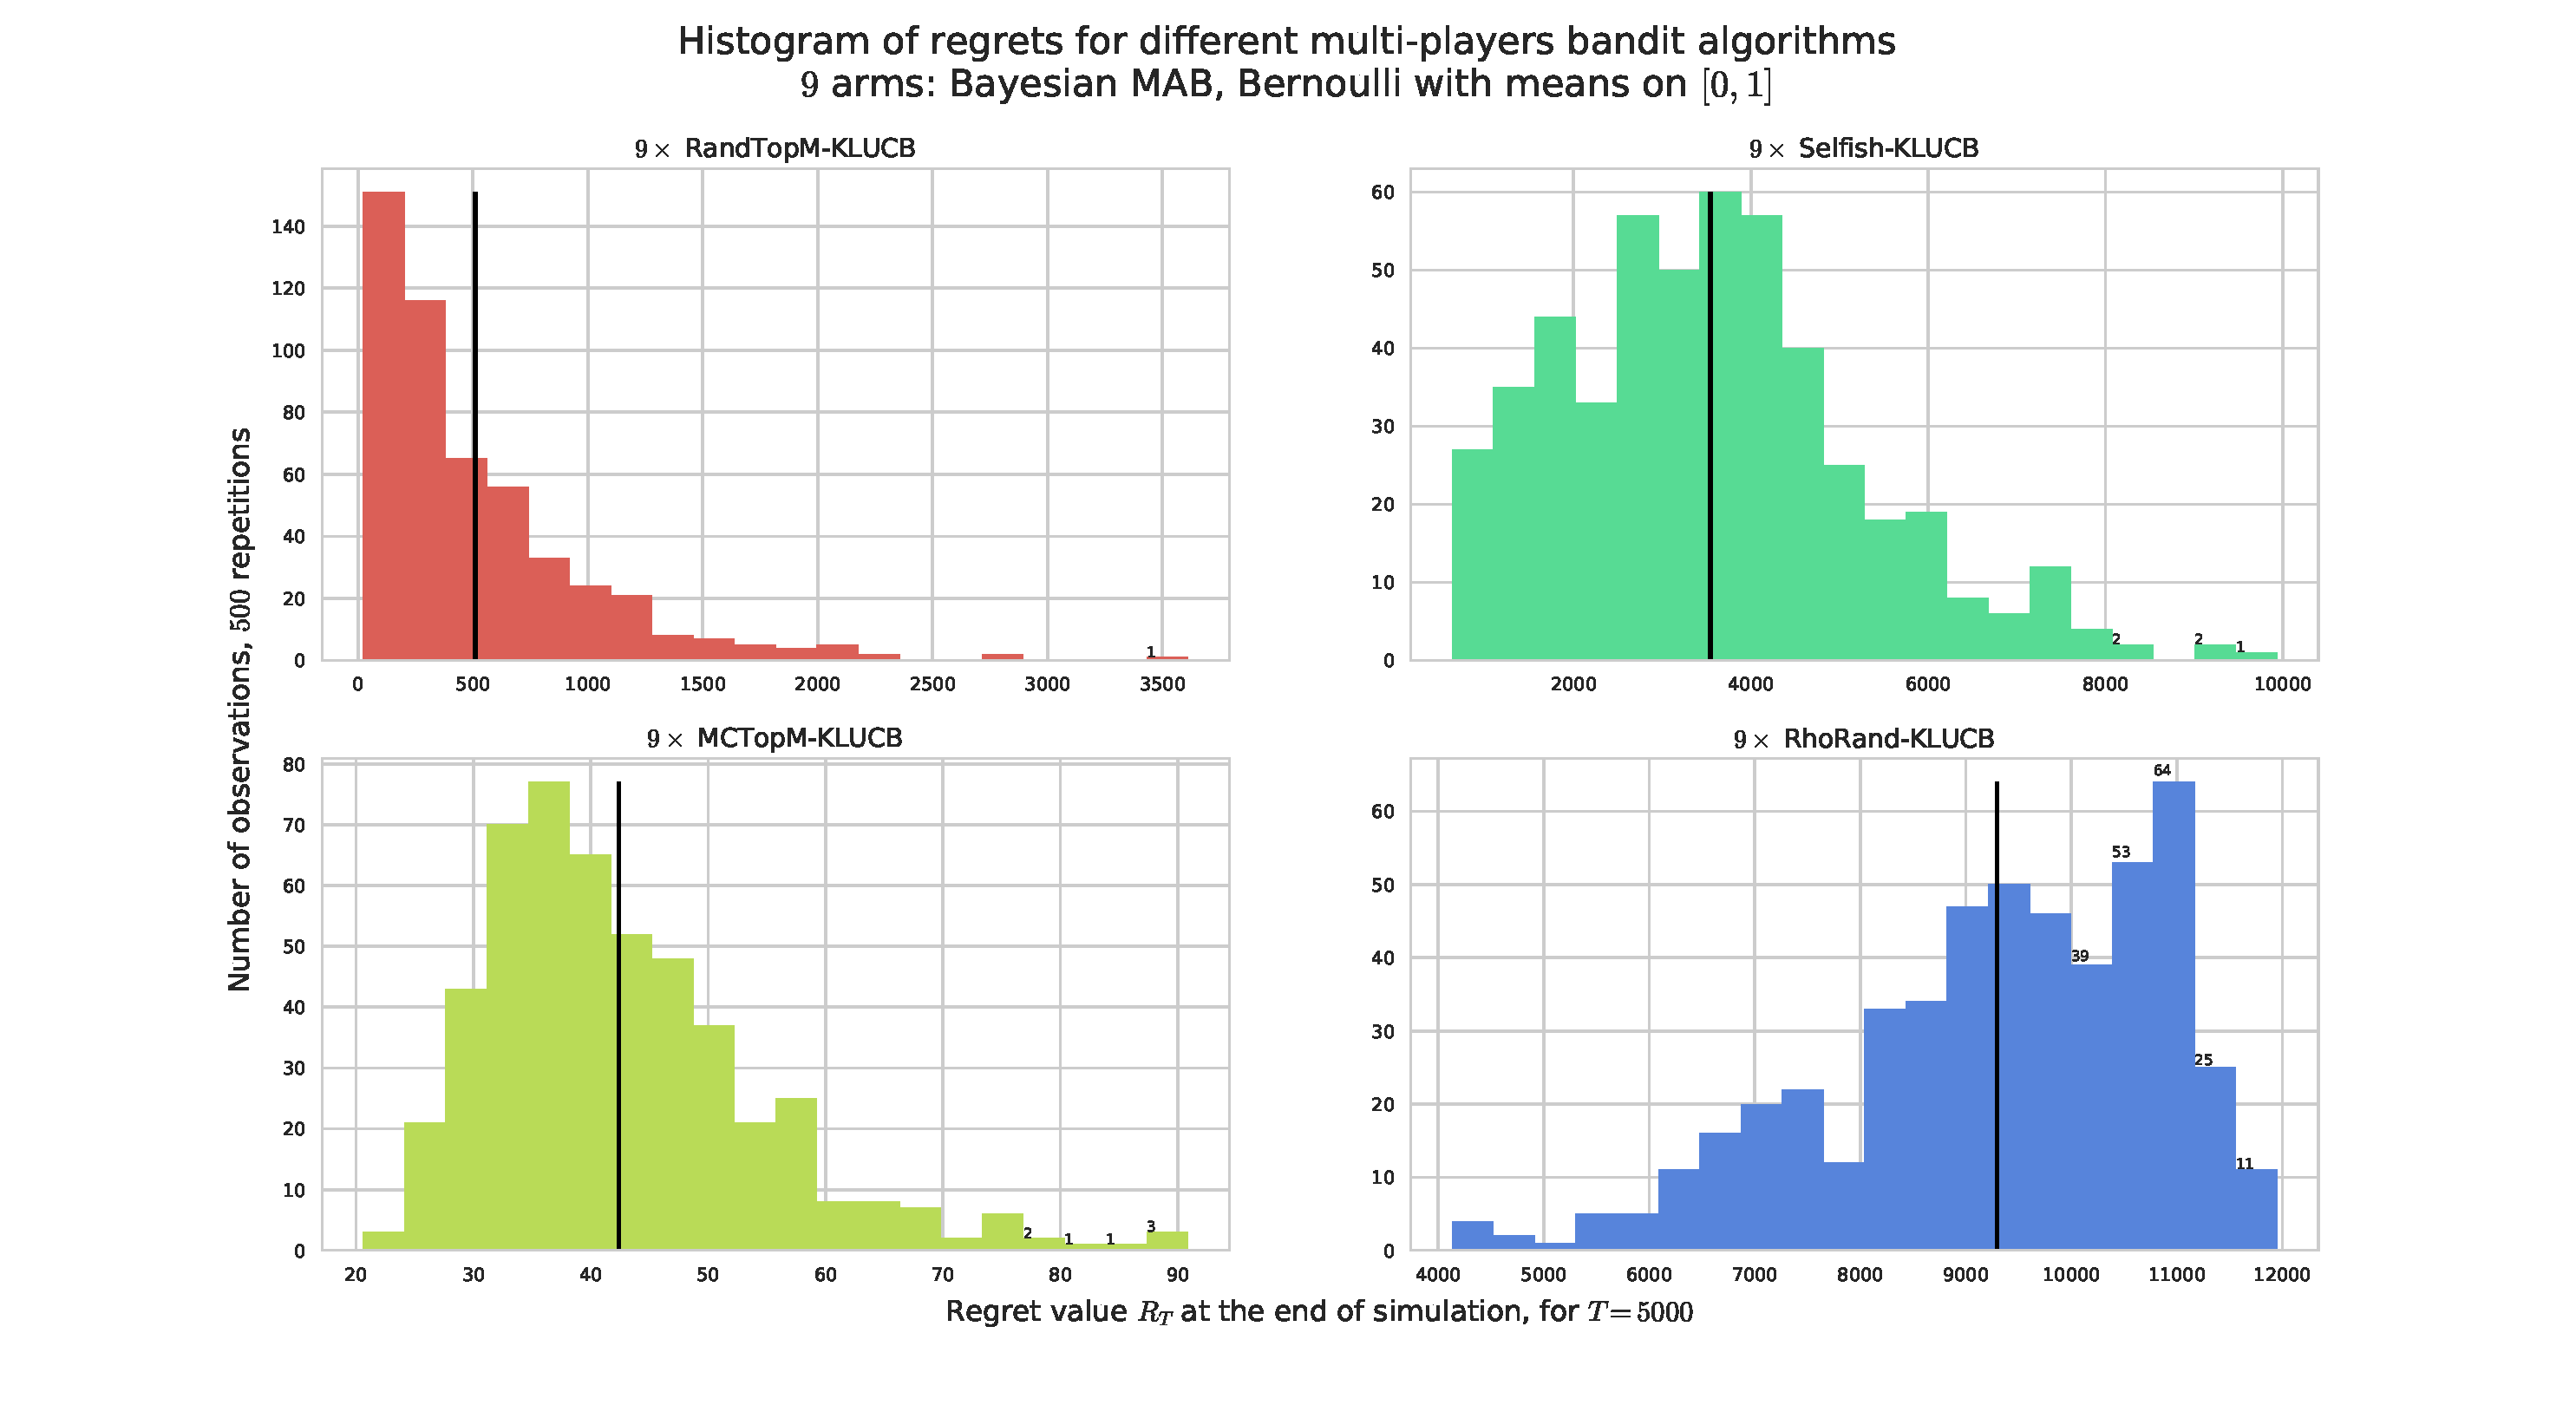
\includegraphics[width=1.00\textwidth]{MP__K9_M9_T5000_N500__4_algos/all_HistogramsRegret____env1-1_3892966382091165662.pdf}
    % \end{subfigure}
    \caption[Regret for $M=9$ players for $K=9$ arms, horizon $T=5000$, against $500$ problems $\boldsymbol{\mu}$ uniformly sampled]{Regret for $M=9$ players for $K=9$ arms, horizon $T=5000$, against $500$ problems $\boldsymbol{\mu}$ uniformly sampled in $[0,1]^K$. This extreme case $M=K$ shows the drastic difference of behavior between \RandTopM{} and \MCTopM, having constant regret, and \rhoRand{} and \Selfish, having large regret.}
    \label{fig:5:MP__K9_M9_T5000_N500__4_algos__all_HistogramsRegret}
    % \vspace*{-15pt}  % XXX remove if problem
\end{figure}


\begin{figure}[!h]
    \centering
    % \begin{subfigure}[!h]{1.00\textwidth}
        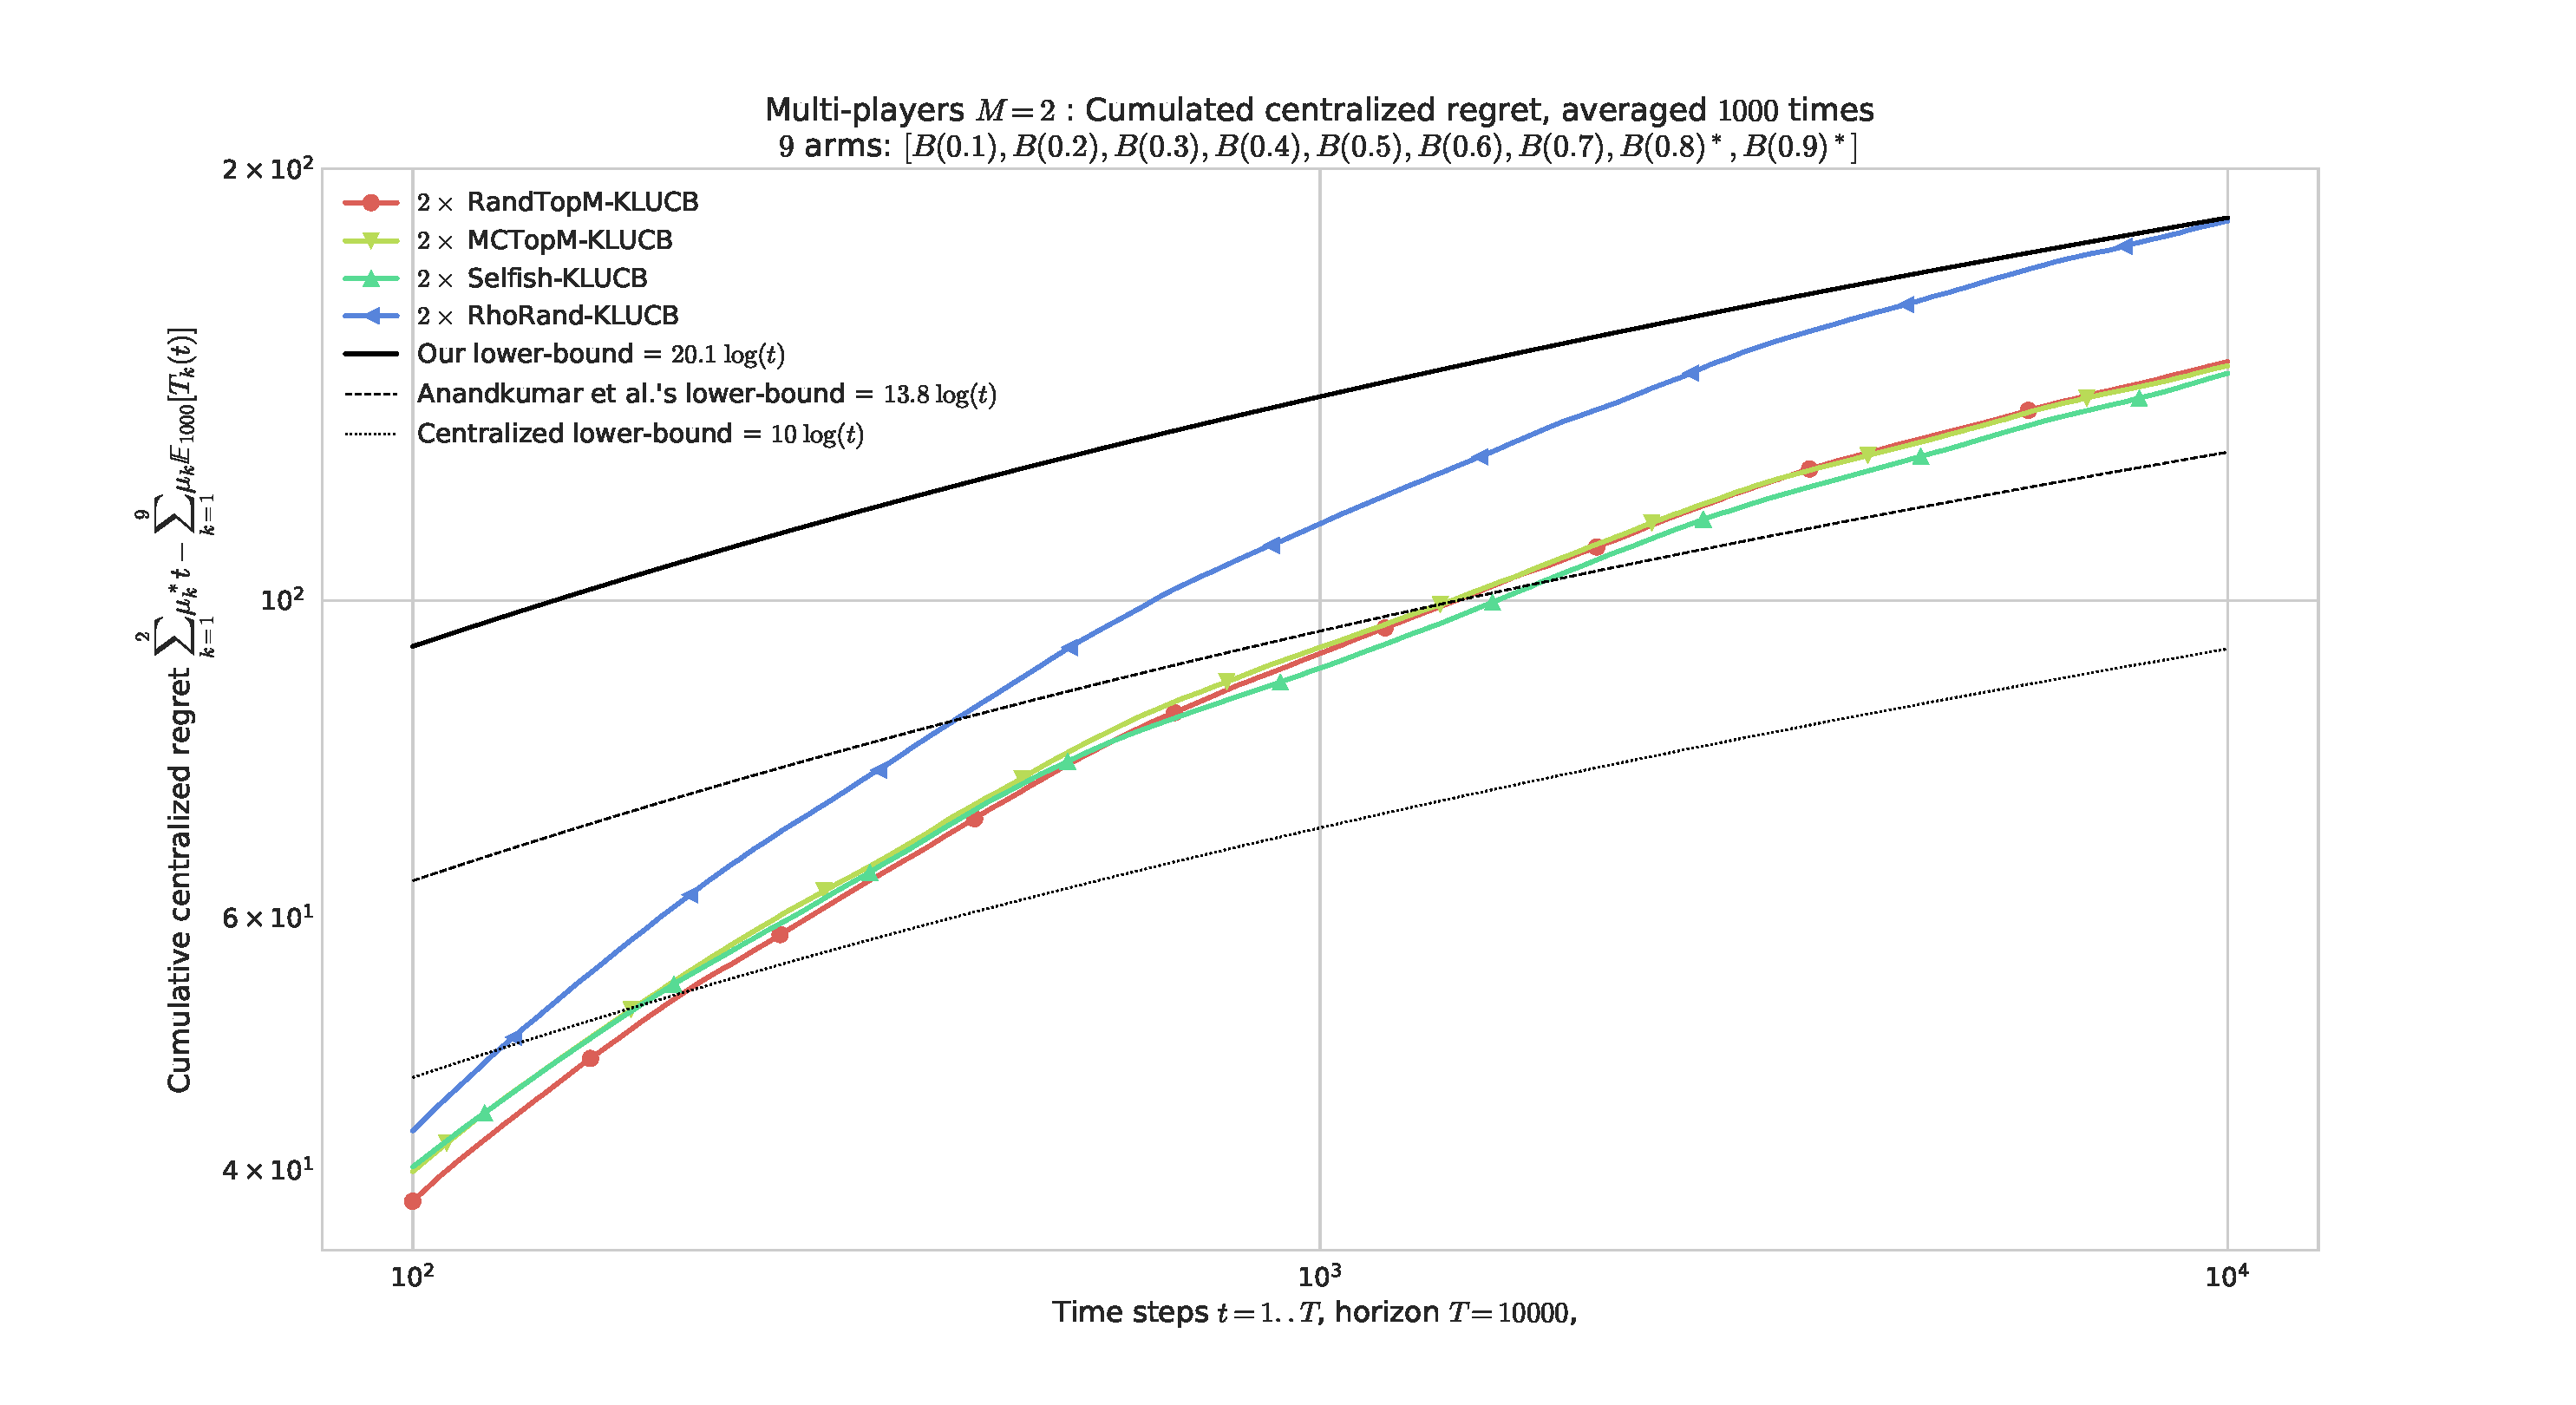
\includegraphics[width=1.00\textwidth]{MP__K9_M2_T10000_N1000__4_algos/all_RegretCentralized_loglog____env1-1_2643359116089264295.pdf}
    % \end{subfigure}
    % ~
    % \begin{subfigure}[!h]{1.00\textwidth}
    %   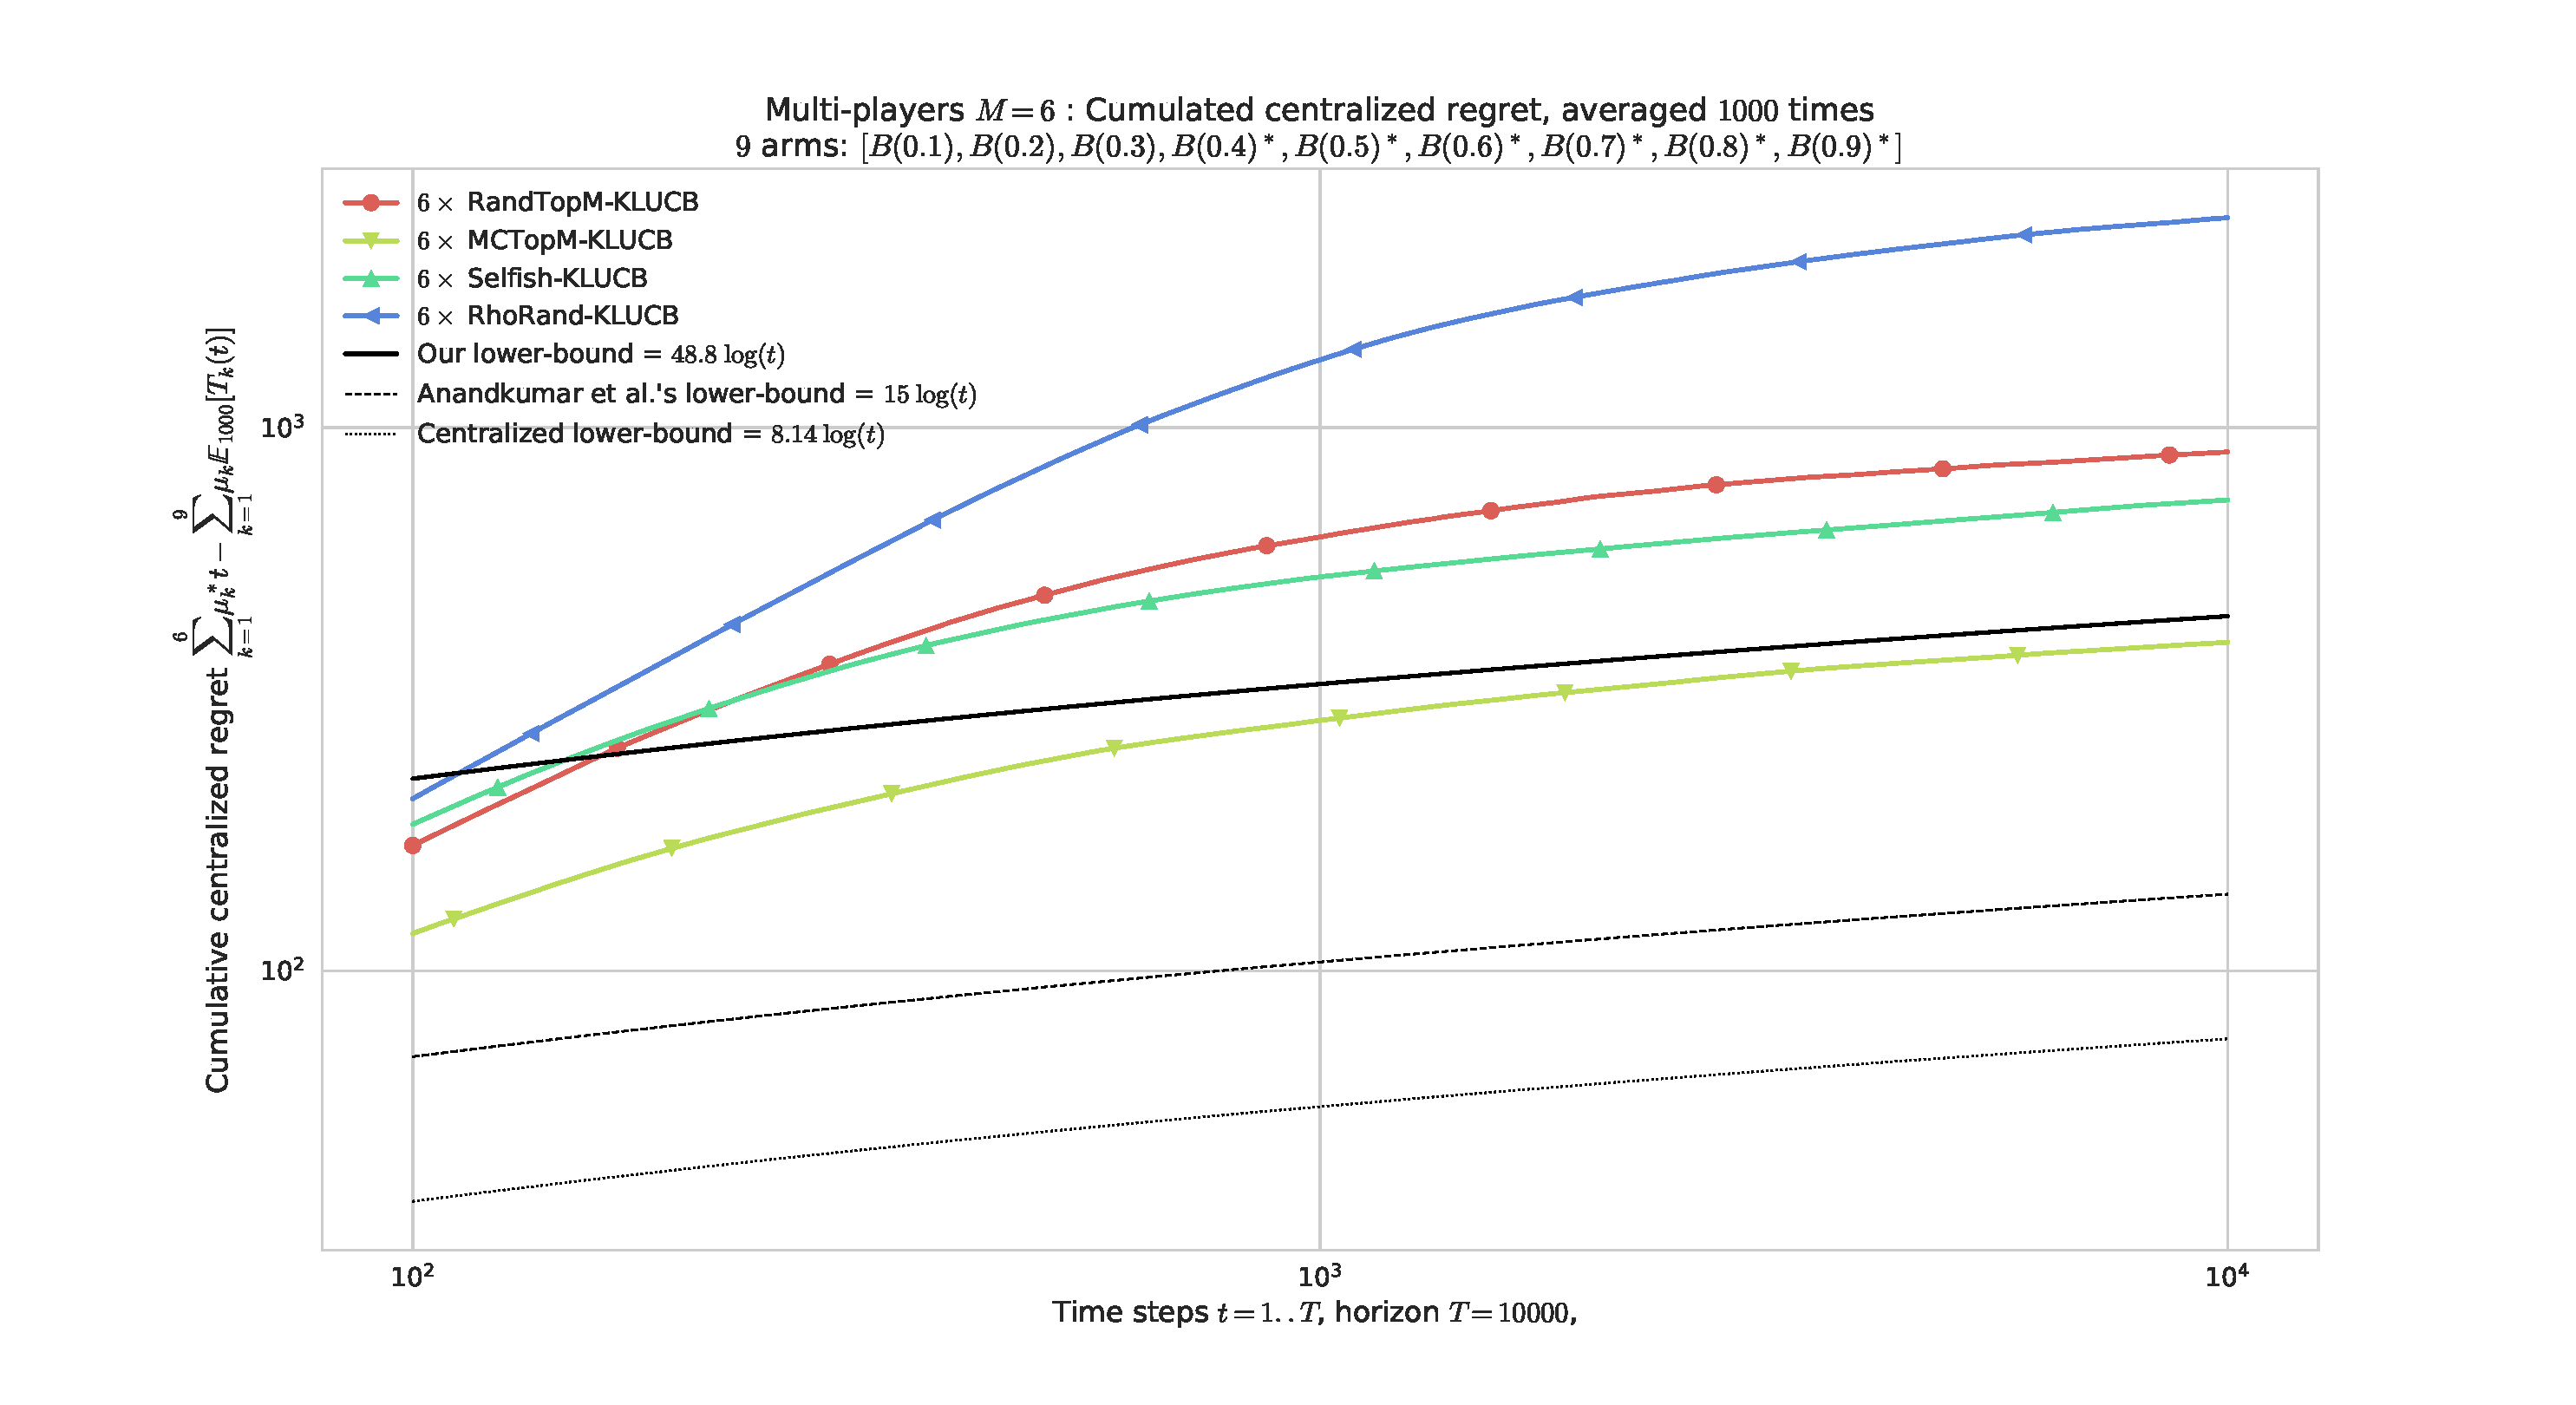
\includegraphics[width=1.00\textwidth]{MP__K9_M6_T10000_N1000__4_algos/all_RegretCentralized_loglog____env1-1_8200873569864822246.pdf}
    % \end{subfigure}
    % ~
    % \begin{subfigure}[!h]{1.00\textwidth}
        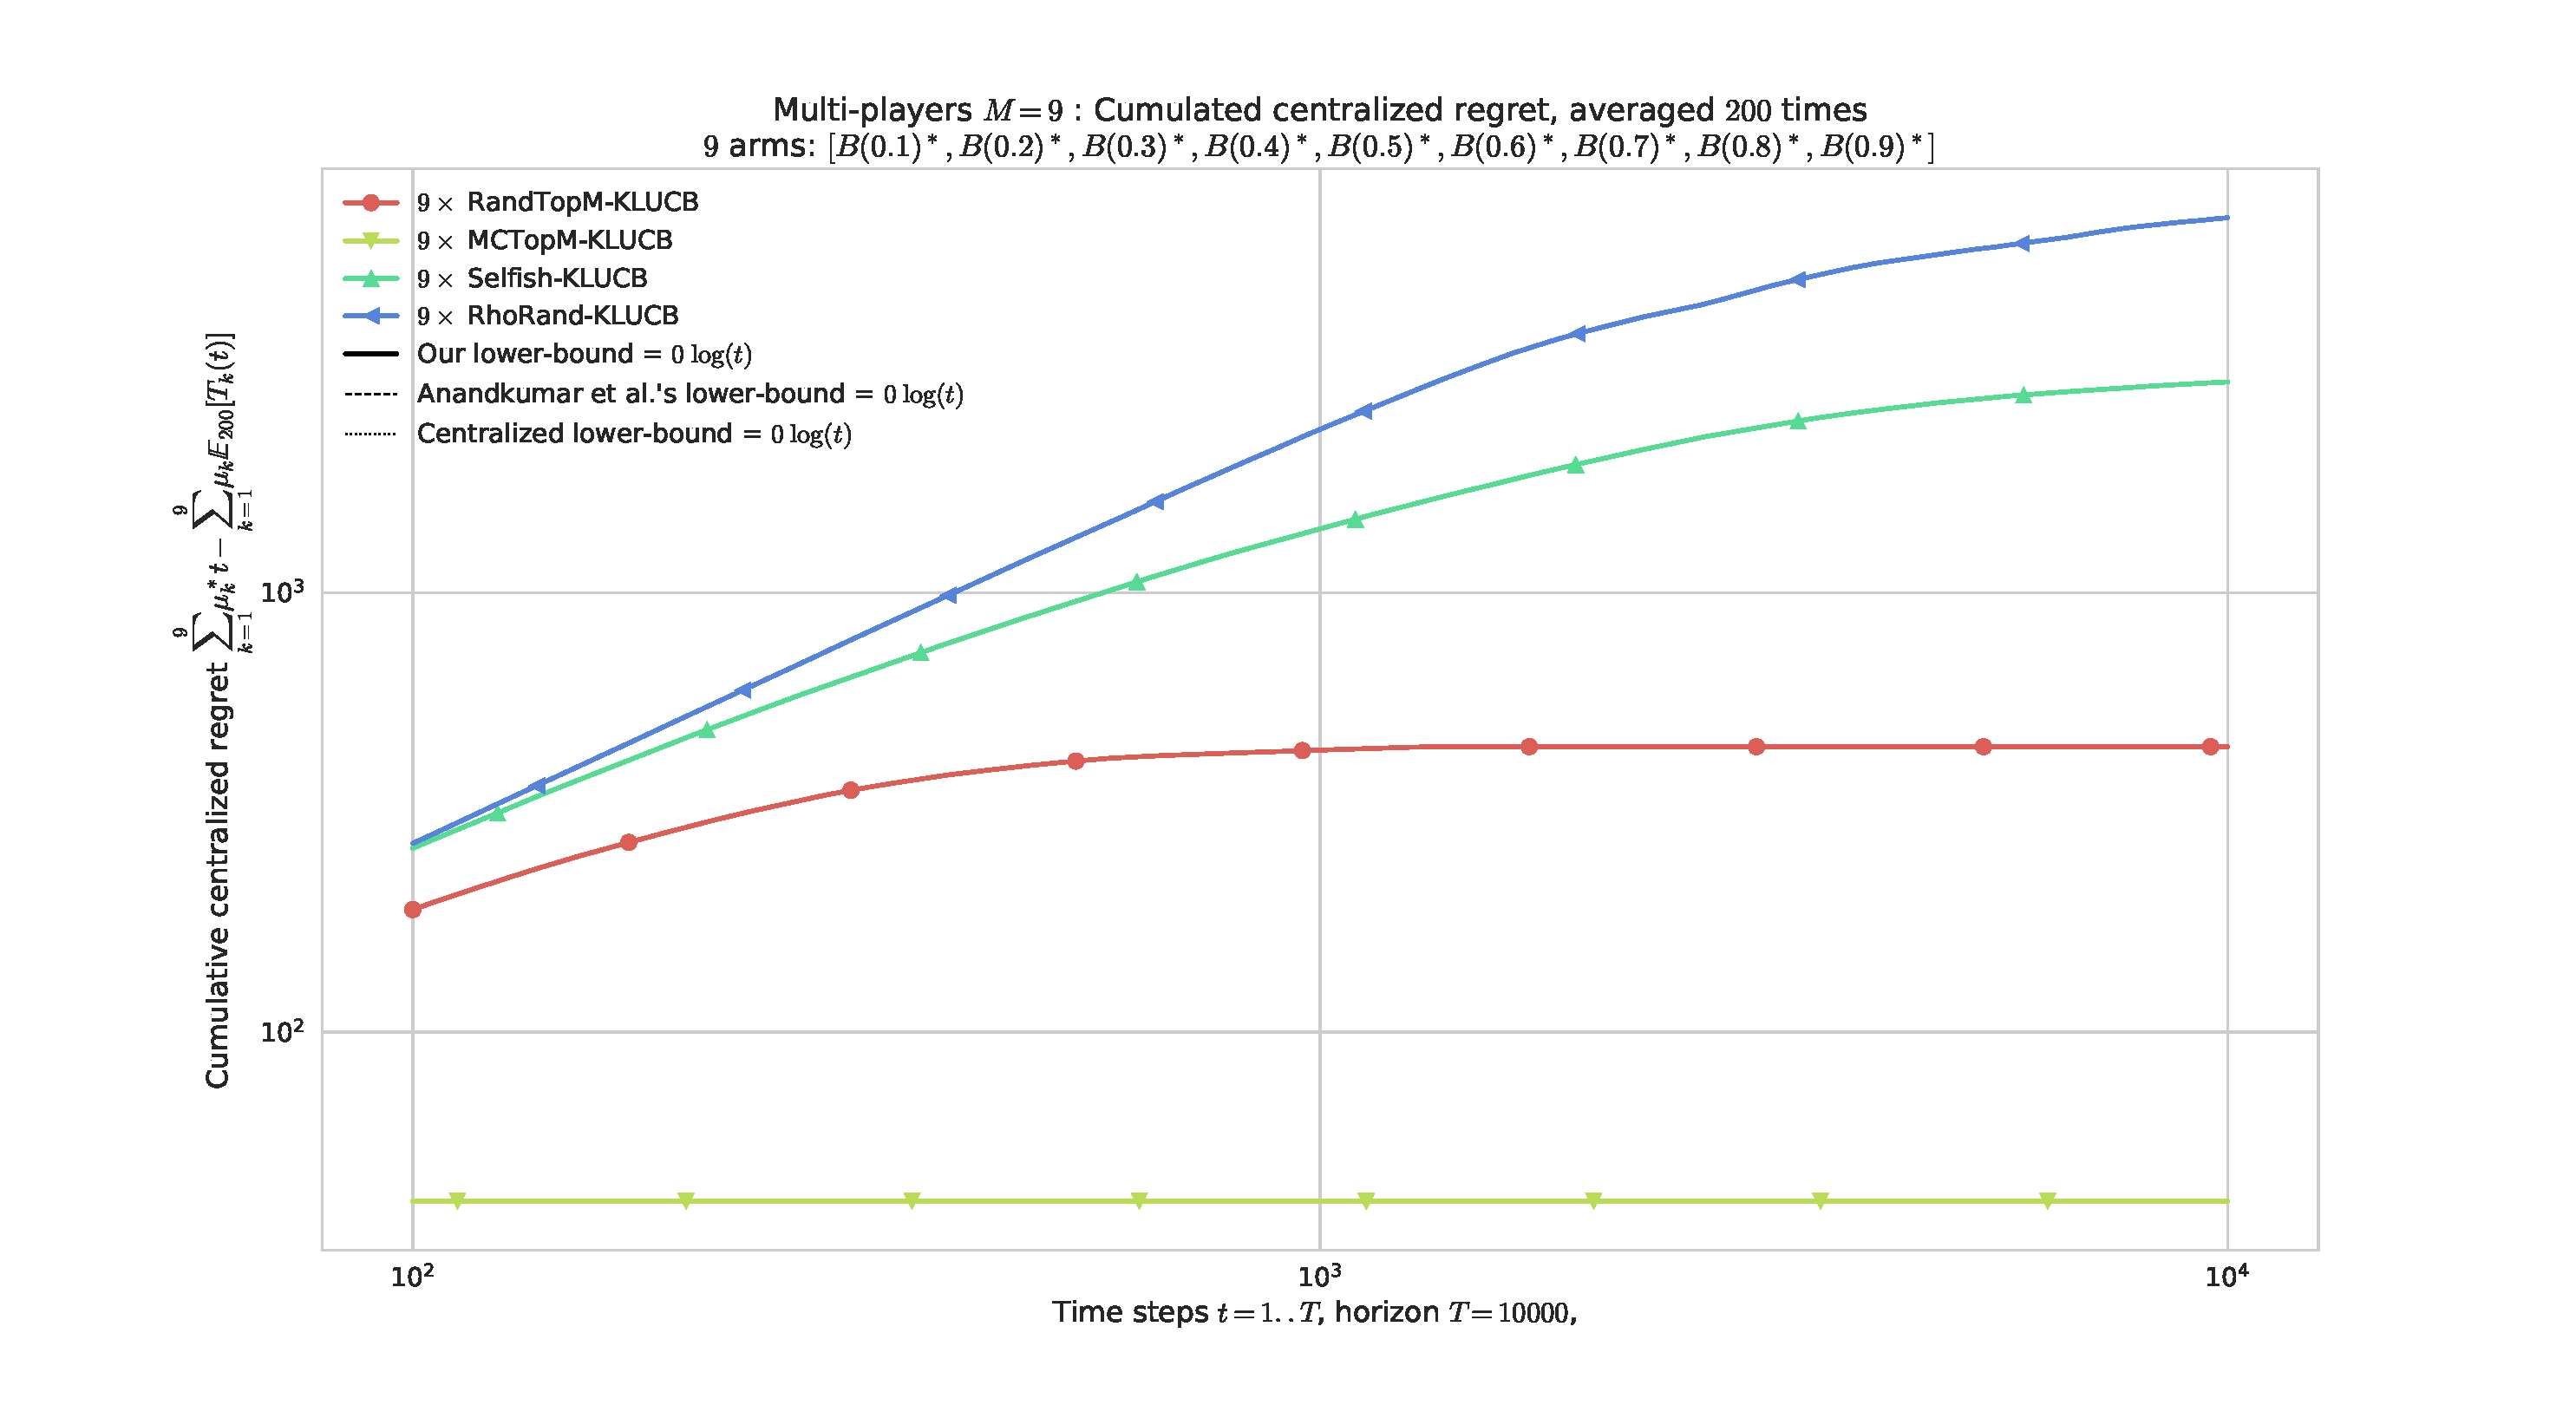
\includegraphics[width=1.00\textwidth]{MP__K9_M9_T10000_N200__4_algos/all_RegretCentralized_loglog____env1-1_2306423191427933958.pdf}
    % \end{subfigure}
    \caption[Regret for $M=2$ and $9$ players for $K=9$ arms, horizon $T=5000$, for a fixed problem]{Regret (in log-log scale), for $M=2$ and $9$ players for $K=9$ arms, horizon $T=5000$,Regret (in log-log scale), for $M=2$ and $9$ players for $K=9$ arms, horizon $T=5000$, for problem $\boldsymbol{\mu}=[0.1,\dots,0.9]$] for problem $\boldsymbol{\mu}=[0.1,\dots,0.9]$. In different settings, \RandTopM{} (\textcolor{gold}{yellow} curve) and \Selfish{} (\textcolor{darkgreen}{green}) can outperform each other, and always outperform \rhoRand. \MCTopM{} is always among the best algorithms, and for $M$ not too small, its regret seems logarithmic with a constant matching the lower bound.}
    \label{fig:5:MP__K9_M2-6-9_T10000_N200__4_algos}
\end{figure}


\begin{figure}[!h]
    \centering
    % \begin{subfigure}[!h]{0.75\textwidth}
        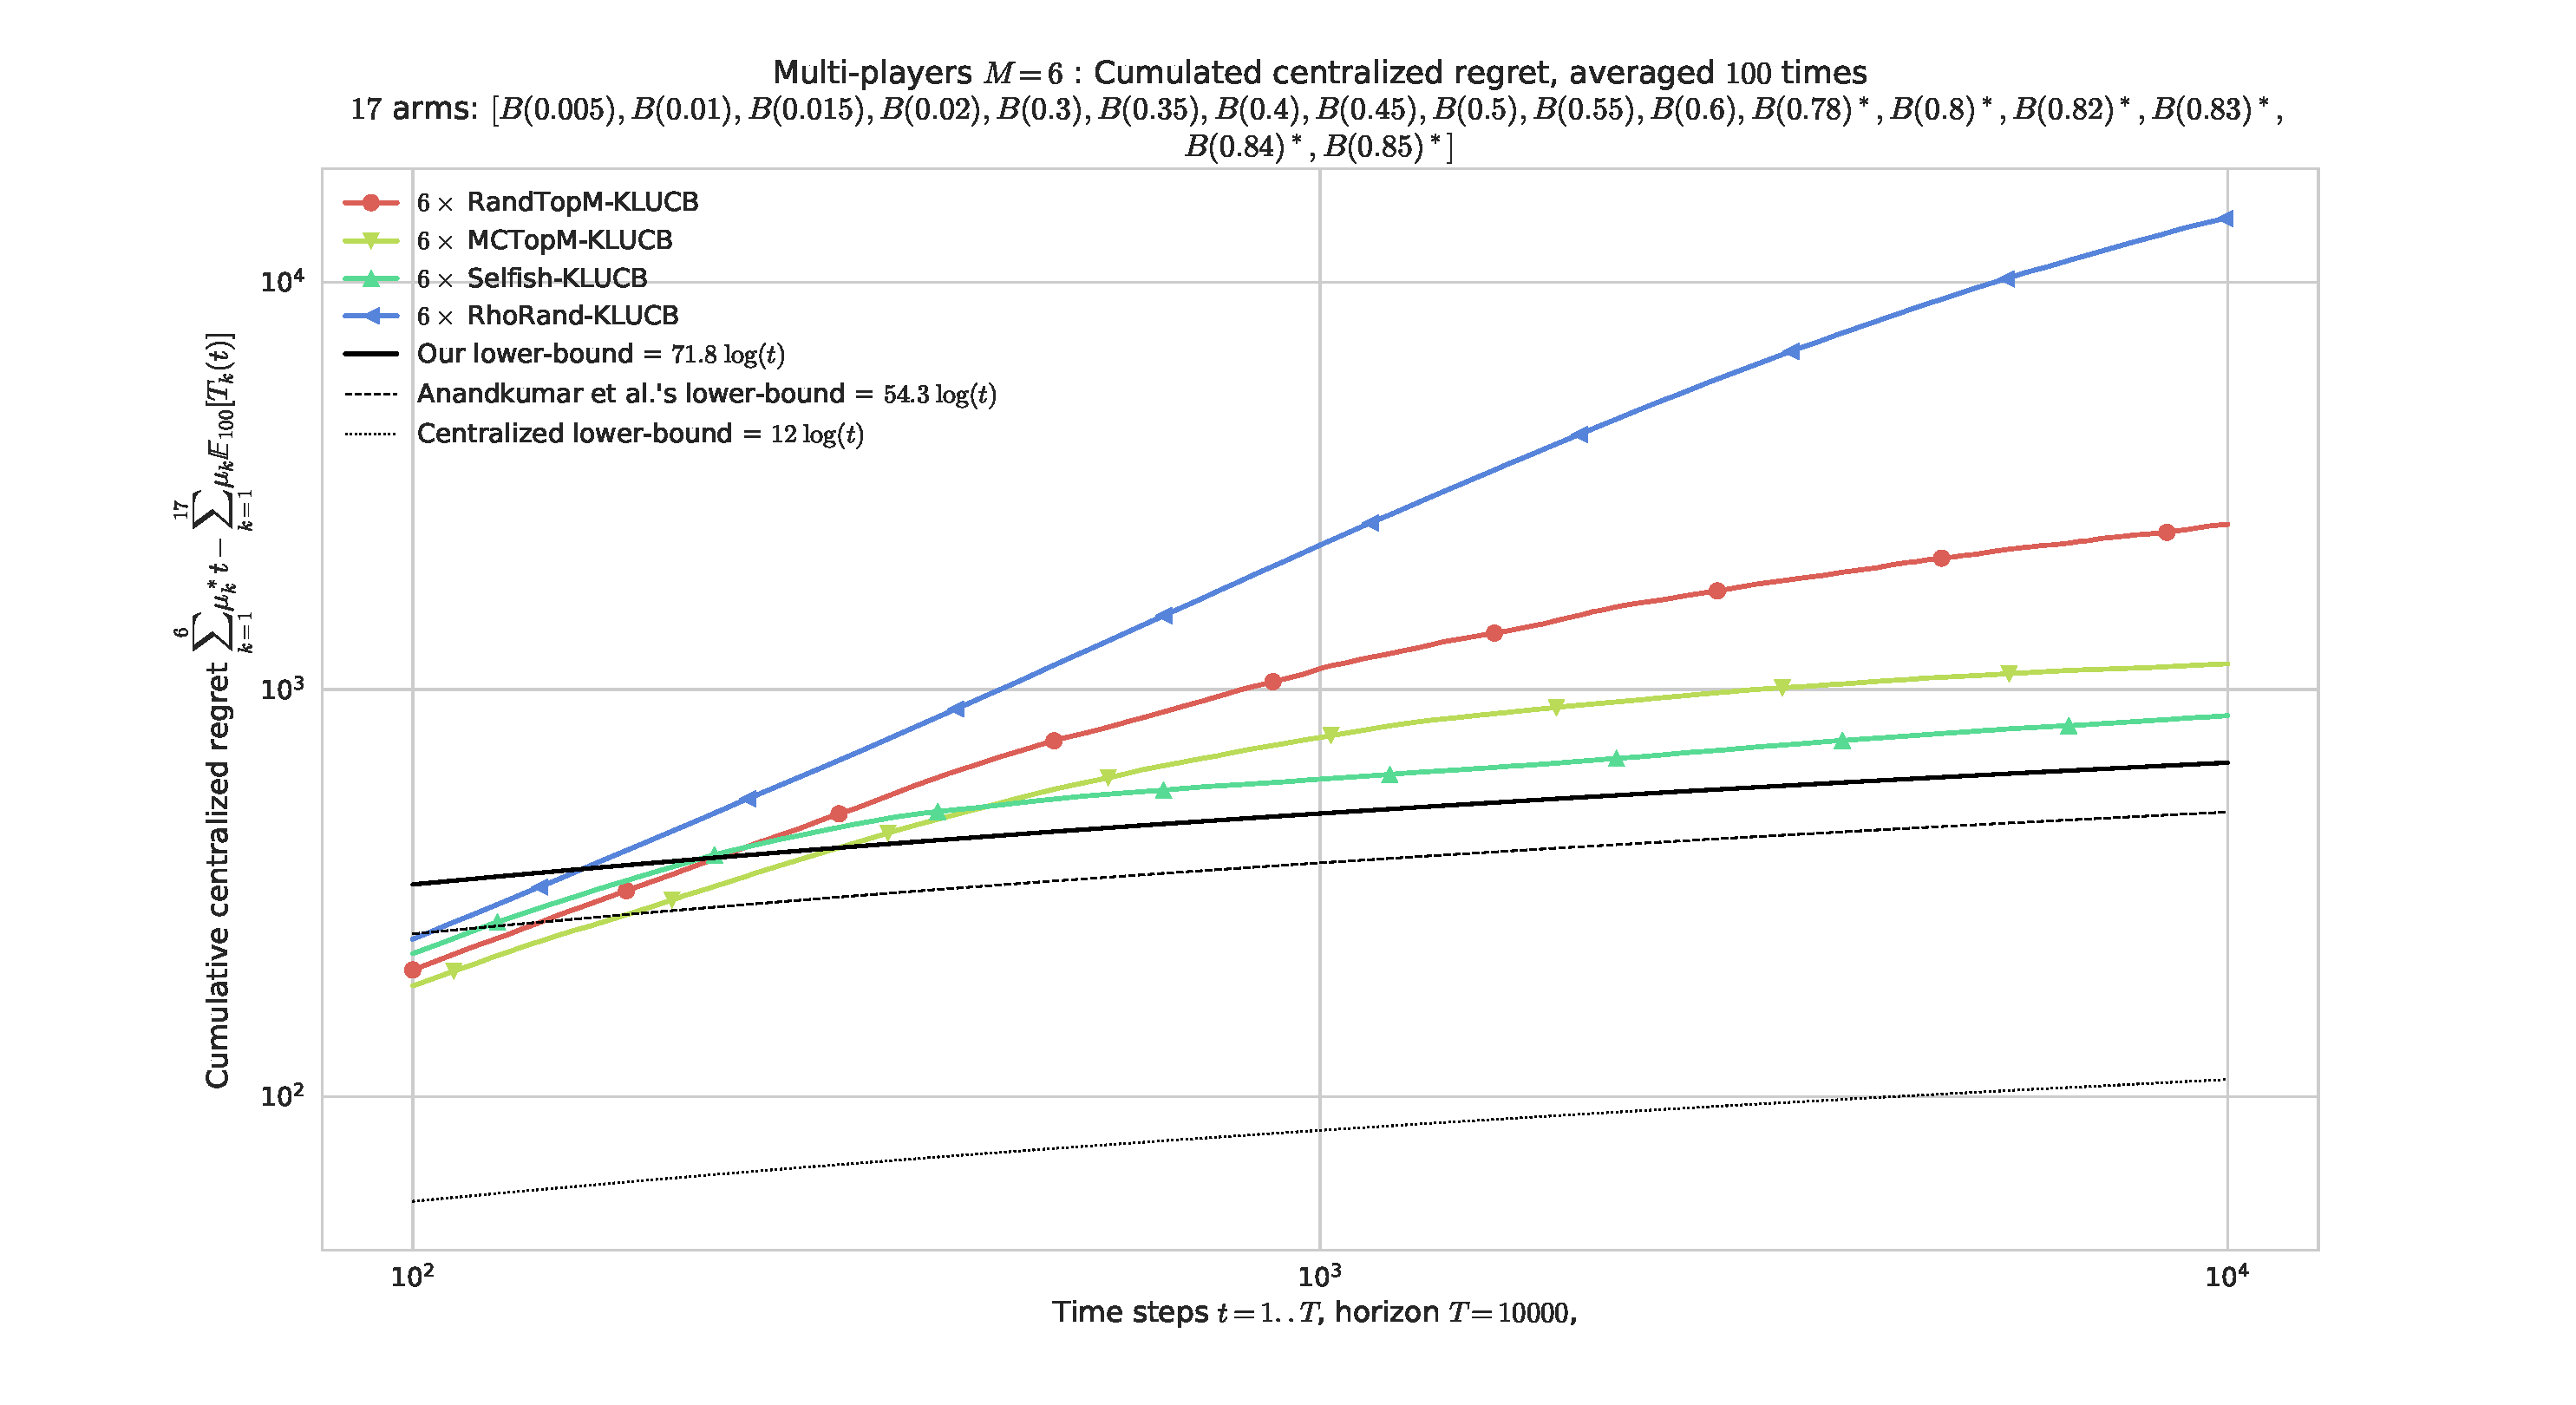
\includegraphics[width=1.00\textwidth]{MP__K17_M6_T10000_N100__4_algos/all_RegretCentralized_loglog____env1-1_4163066365888233475.pdf}
    % \end{subfigure}
    % ~
    % \begin{subfigure}[!h]{0.75\textwidth}
        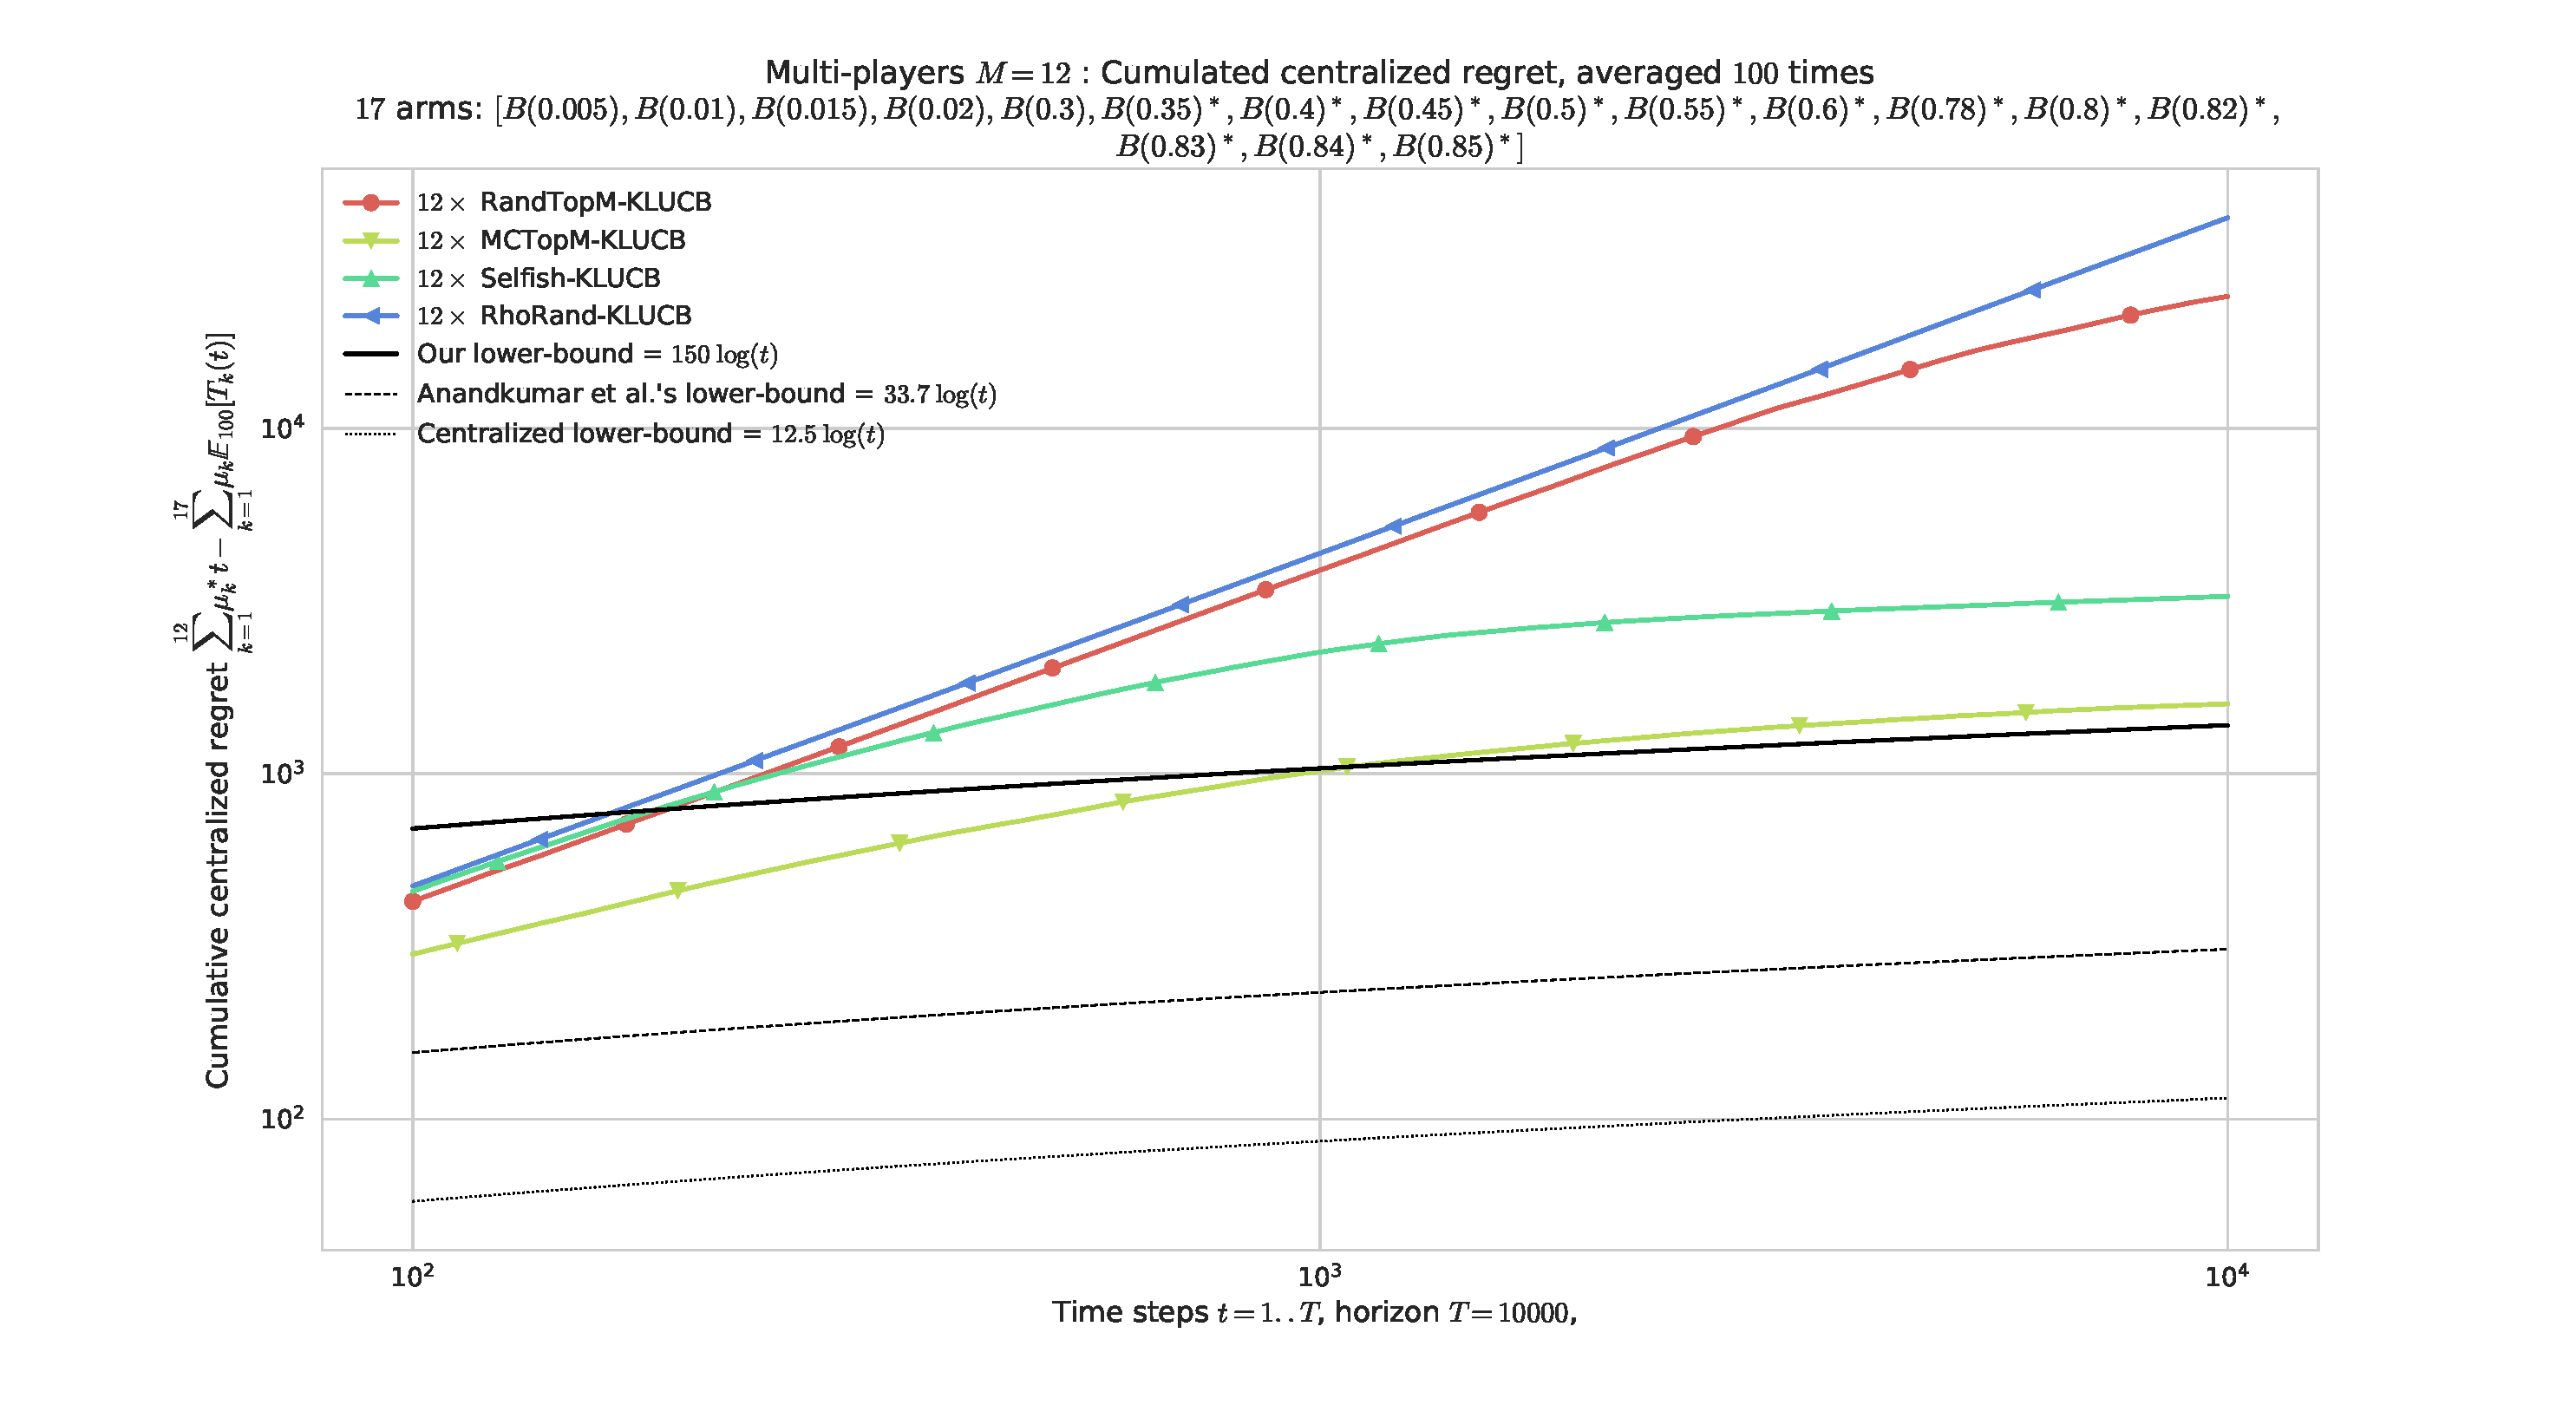
\includegraphics[width=1.00\textwidth]{MP__K17_M12_T10000_N100__4_algos/all_RegretCentralized_loglog____env1-1_3856003705095179548.pdf}
    % \end{subfigure}
    % ~
    % \begin{subfigure}[!h]{0.75\textwidth}
        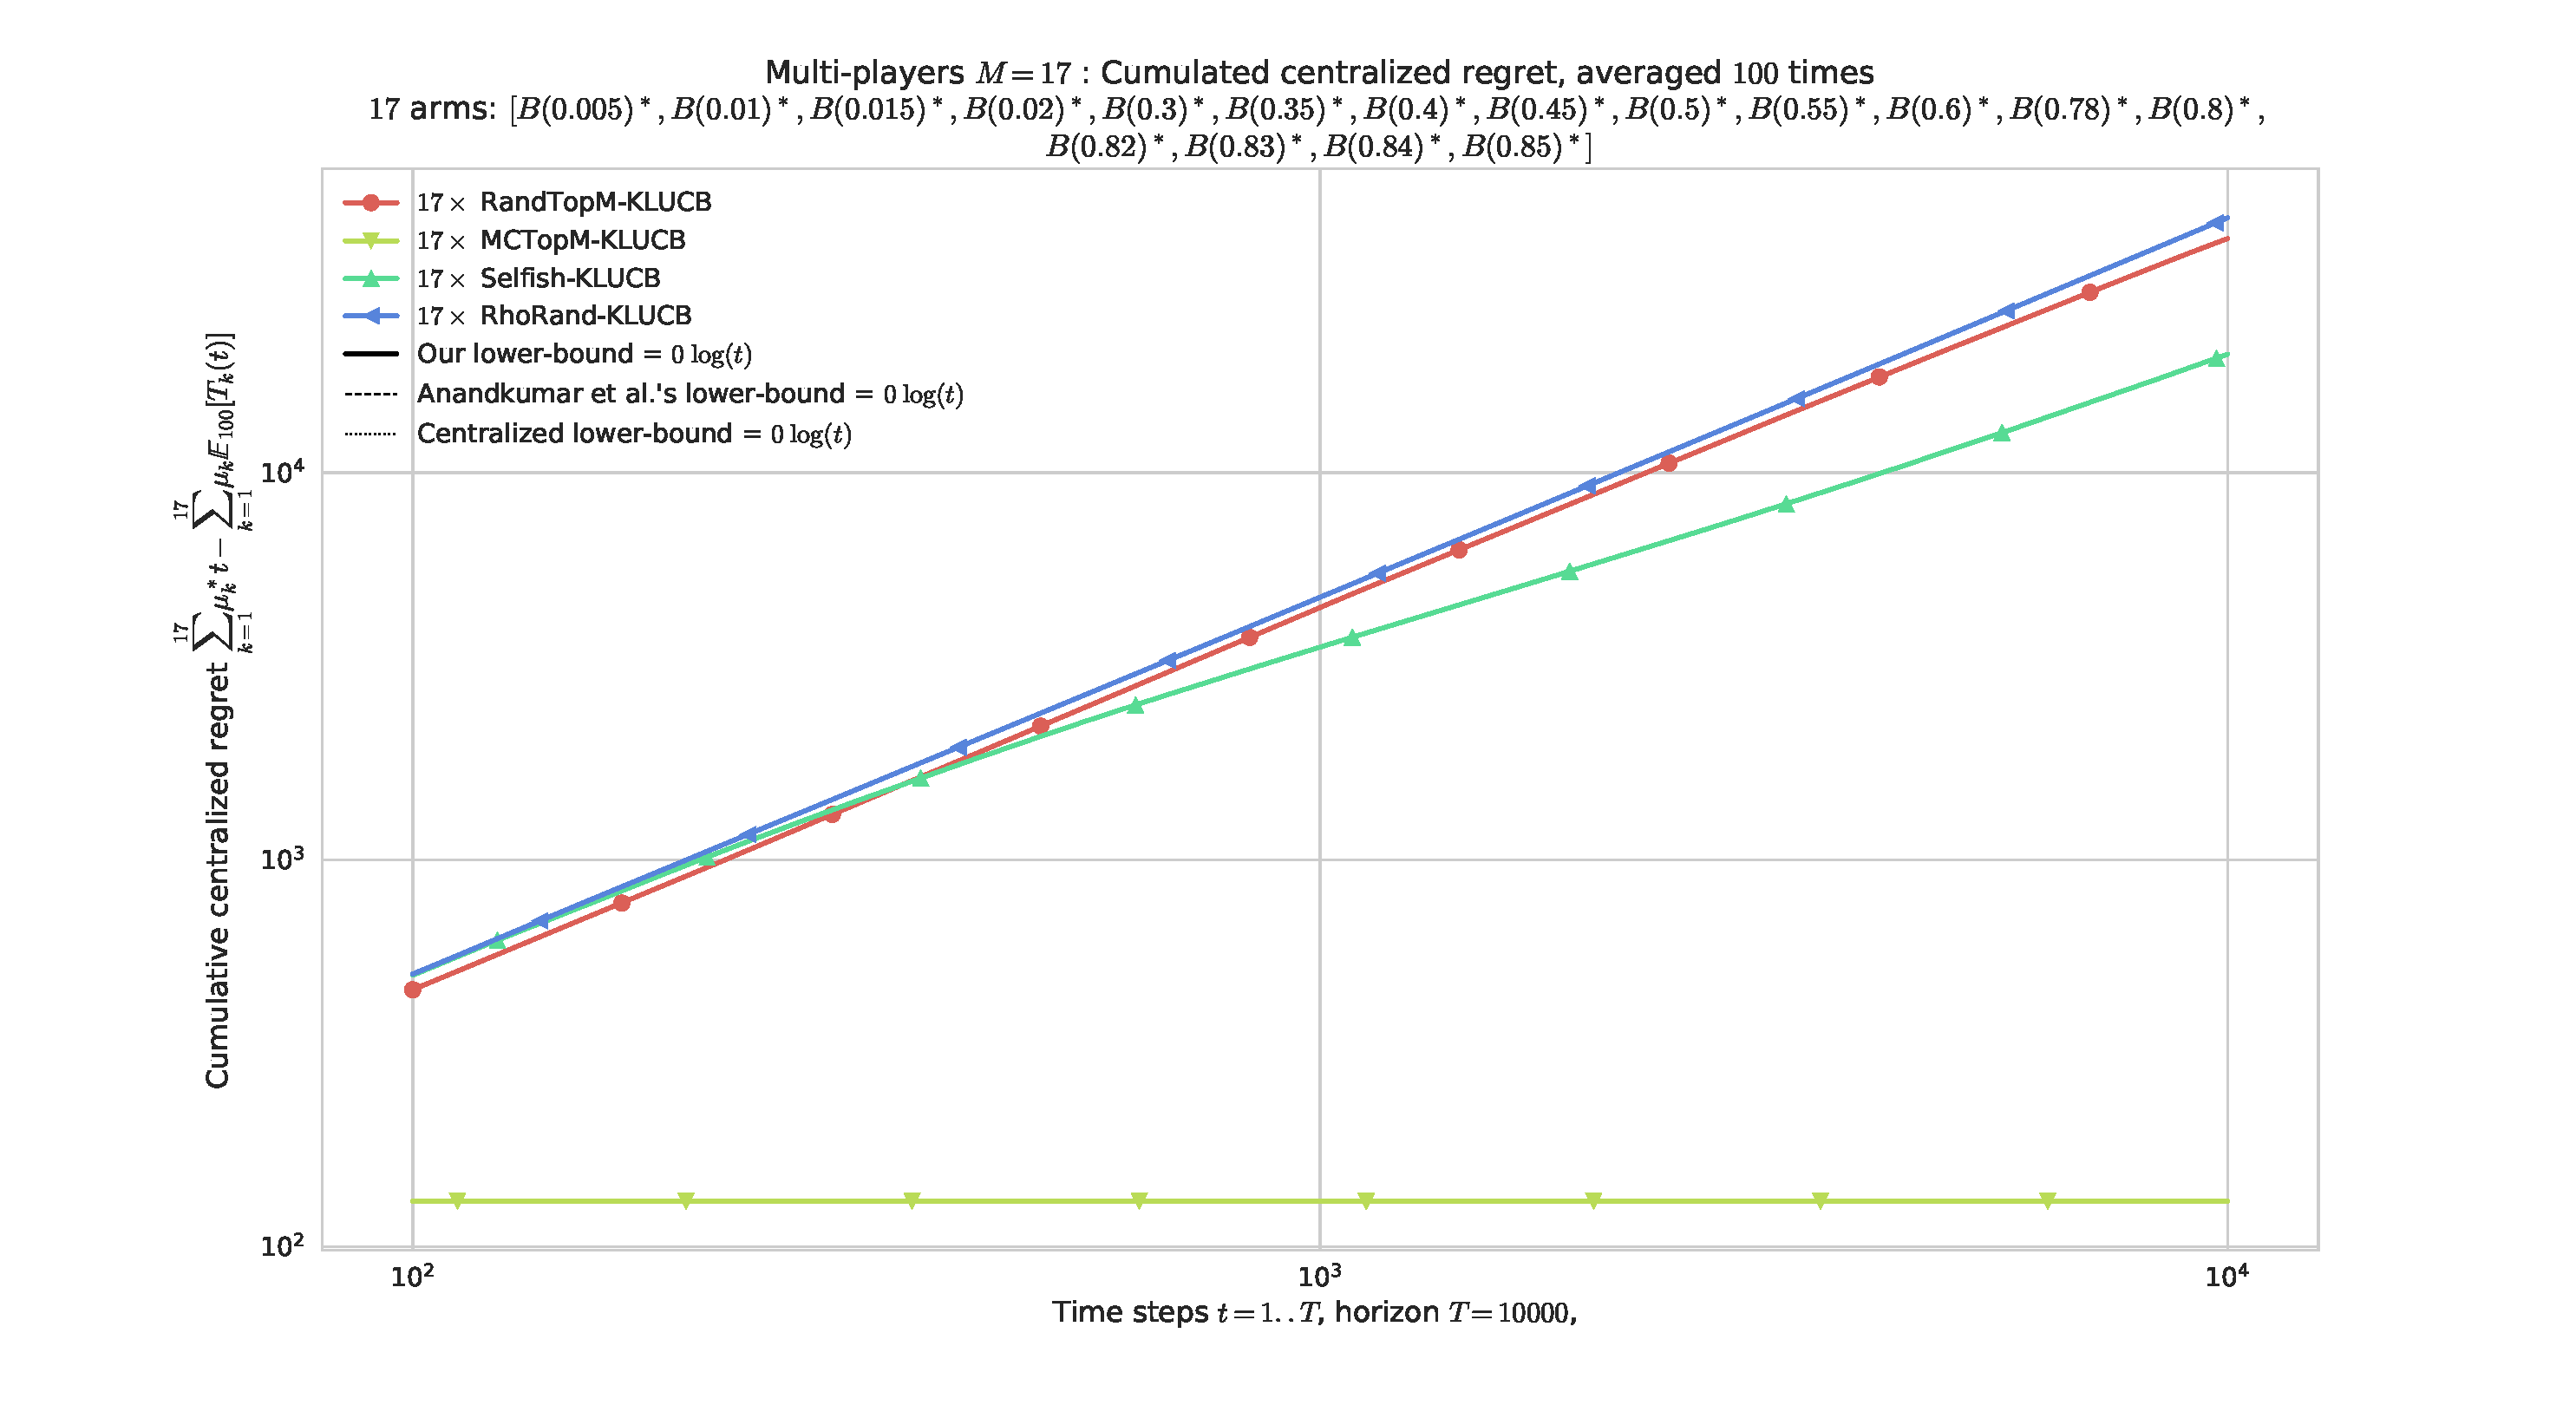
\includegraphics[width=1.00\textwidth]{MP__K17_M17_T10000_N100__4_algos/all_RegretCentralized_loglog____env1-1_8969236287861113966.pdf}
    % \end{subfigure}
    \caption[Regret for $M=6, 12, 17$ players for a ``difficult'' problem with $K=17$, and $T=5000$]{Regret (in log-log scale), for $M=6, 12, 17$ players for a ``difficult'' problem with $K=17$, and $T=5000$. The same observation as in Figure~\ref{fig:5:MP__K9_M2-6-9_T10000_N200__4_algos} can be made. \Selfish{} outperforms \MCTopM{} for $M=2$ here. Additionally, \MCTopM{} is the only algorithm to not fail dramatically when $M=K$ here.}
    \label{fig:5:MP__K17_M6-12-17_T10000_N100__4_algos}
\end{figure}


